% !TeX program = lualatex
% !TeX encoding = UTF-8
% !TeX spellcheck = fr_FR

\documentclass[12pt]{report}

%%%%% PREAMBULE %%%%%
%%% Langue
\usepackage{polyglossia} %Langue
\setmainlanguage{french}
\setotherlanguage{english}

%%% Aspect Documents
\usepackage{geometry}
\geometry{a4paper,
			twoside,
			top=2.5cm,
			bottom=2.5cm,
			left=2.5cm,
			right=2.5cm}
\setlength{\marginparwidth}{2cm}%Marge de 2cm a gauche et a droite dans retrait de 2.5cm. Pour meileur affichage \todo.

%%% Police / Présentation
\usepackage{fontspec} %Police
\setmainfont[Ligatures=TeX,
			Kerning=Uppercase, %Meilleurs intégration Maj-Min
			BoldFont={AGaramondPro-Bold},
			ItalicFont={AGaramondPro-Italic},
			Numbers=Proportional,]{Adobe Garamond Pro} %test
\usepackage{microtype}
\usepackage{unicode-math} %Plante si absent mais formule dans texte
\setmathrm{Adobe Garamond Pro}
%\usepackage[adobe-garamond]{mathdesign} %Police signe maths %%Fait buguer avec unicode-math
\usepackage[version=4]{mhchem} %Ecriture ion/molécules
\usepackage[artemisia]{textgreek}
\usepackage{multicol}
\usepackage{ulem} %Soulignement, barré etc

%%% Présentation
\usepackage{csquotes}
\usepackage{parskip}
\setlength{\parindent}{3em}
\usepackage{caption} %Titre figure mieux géré
\captionsetup{%justification=raggedright, 
			singlelinecheck=false}
\usepackage{subcaption} %idem sous figures
\usepackage{threeparttable}
\usepackage{titlesec}
\usepackage{titling} %Utilisation titre dans en-tête
\usepackage{xspace} %Gestion espace dans macro
\usepackage{fancyhdr} %Gestion en-tête et pieds de page
\fancypagestyle{plain}{ %Redef style page plain de page avec Chapitre
	\fancyhf{} % clear all header and footer fields
	\fancyhead[C]{\textit{\titredoc}}
	\fancyfoot[C]{\textbf{\thepage}} % except the center
	\renewcommand{\headrulewidth}{0,4pt}
	\renewcommand{\footrulewidth}{0pt}}
\setlength{\headsep}{25pt}

%%% Pasde chgt de page nouveau chapitres
\usepackage{etoolbox}
\makeatletter
\patchcmd{\chapter}{\if@openright\cleardoublepage\else\clearpage\fi}{}{}{}
\makeatother

%%% Images & figures
\usepackage{graphicx} %Gestion des images
\usepackage{wrapfig} %Gestion des images, permet mise image et texte cote a cote
\usepackage{placeins}
	%%%Figure
\captionsetup[figure]{labelfont={bf}, labelformat={default}, labelsep=period, name={Figure }} %Affichage Figure x. au lieu de fig x. dans figure
\captionsetup[table]{labelfont={bf}, labelformat={default}, labelsep=colon, name={Table }} %idem pour table
	%%%Sous Figure
\captionsetup[subfigure]{labelformat=simple}
\renewcommand{\thesubfigure}{\Alph{subfigure}}
\DeclareCaptionLabelFormat{bold}{\textbf{(#2)}}
\captionsetup{subrefformat=bold}
\renewcommand{\thefigure}{\arabic{figure}} %Permet "Figure X" au lieu de "Figure Y.X" (Y étant num chapitre, X num figure)
\renewcommand{\thetable}{\arabic{table}}

\usepackage{chngcntr}
\counterwithout{figure}{chapter} %Compteur continu entre chapitre

%%% Pdf / Références internes
\usepackage{hyperref} %Meilleure gestion pdf, load avant glossaries pour crossref
\hypersetup{pdfauthor={Florent KLEE},
	pdftitle={Roles de Wnts et MuSK, un récepteur tyrosine kinase dans le cerveau},
	pdfsubject={Roles de Wnts et MuSK dans le cerveau},
	colorlinks,
	citecolor=black,
	filecolor=black,
	linkcolor=black,
	urlcolor=gray,}
\usepackage{fancyref} %Après Hyperef
\usepackage{cleveref} %Ref mieux gérer
\newcommand{\crefpairconjunction}{ et } %"figs x et y" au lieu de "figs x and y"
\newcommand{\crefrangeconjunction}{ à } %figs x à y au lieu de figs x to y

\providecommand\phantomsection{}% for hyperref

%%% Glossaire
%\usepackage{glossaries}
\usepackage[
			toc,
			nogroupskip,
			nonumberlist,%Pas de numéro de pages
			acronym,
			nopostdot,
			]{glossaries}
\newacronymstyle{twocollist}%
	{%
		\GlsUseAcrEntryDispStyle{long-short}%
	}%
	{%
		\GlsUseAcrStyleDefs{long-short}%
		\renewcommand*{\GenericAcronymFields}{description={\capitalisewords{\the\glslongtok}}}%
		\BeforeBeginEnvironment{theglossary}{\begin{multicols*}{2}}
		\AfterEndEnvironment{theglossary}{\end{multicols*}}
	}
\renewcommand{\glossarypreamble}{\small}
\setacronymstyle{twocollist}
\makeglossaries

%%% Biblio
\usepackage[sorting=none,
			backend=biber,
			style=FKStyle,
			datamodel=FKStyledata,
			block=none,
			date=year,
			minbibnames=3, maxbibnames=9,
			]{biblatex} %A voir + tard
\addbibresource{library.bib}
\defbibheading{subbibliography}[\refname]{\section*{#1}}
\usepackage[nottoc]{tocbibind} %Bibliographie dans Table des matières

%%% Divers
\usepackage{todonotes}

%%% Création Index
\makeindex

%Redef format section (chapite, chapitre* et paragraph), notamment reduire espace au dessus et dessous de ceux ci
%Depend du package Titlesec
%\titleformat{command}[shape]{format}{abel}{sep}{before-code}[after-code]
%\titleformat{\chapter}[hang]{\normalfont\LARGE\bfseries}{\chaptertitlename~\thechapter : }{17\p@}{\LARGE}
\makeatletter
\titleformat{\chapter}[hang]{\normalfont\LARGE\bfseries}{\thechapter) }{5\p@}{\LARGE}
\titlespacing*{\chapter}{0pt}{10\p@}{13\p@}
\titleformat*{\section}	{\normalfont\Large\bfseries}
\titlespacing*{\section}{0pt}{3\p@}{5\p@}
\titleformat{\paragraph}[runin]{\normalfont\normalsize\bfseries}{}{0\p@}{}[.]
\makeatother

%%%%% COMMANDES / MACRO %%%%%
\newcommand{\blankpage}{\newpage\thispagestyle{empty}\null\newpage} %Création page blanche
\newcommand{\up}[1]{\textsuperscript{#1}} %Permet exposants
\newcommand{\mcrd}{MuSK\textDelta{}CRD\xspace} %Ecrire MuSK-CRD
\newcommand{\titredoc}{Rôles de Wnts et MuSK,\\un récepteur tyrosine kinase dans le cerveau }
\newcommand{\teteCol}[1]{\multicolumn{1}{c}{#1}}
\newcommand{\descfig}[1]{\footnotesize{#1}}

%%%%% GLOSSAIRE %%%%%
\loadglsentries{./Glossaire.tex}

%%%%%%%%%% DOCUMENT %%%%%%%%%%
\begin{document}
\normalem %Empeche modif de \emph{} par package ulem
\pagestyle{fancy}
\fancyhf{}
\chead{\textit{\titredoc}}

%%%%% Page de Garde %%%%%	
\begin{center}

%%%%% LOGO %%%%%
\begin{figure}[!h] %!h = en haut ! 
	\begin{minipage}{0.48\textwidth}
		\raggedright %Tout a gauche
		\includegraphics*[height=0.1\textheight]{./Images/Logo_P5.png}
	\end{minipage}%	
	\hfill
	\begin{minipage}{0.48\textwidth}
		\raggedleft %Tout a droite
		\includegraphics*[height=0.1\textheight]{./Images/Logo_CNRS.png}
	\end{minipage}%
\end{figure}
\vspace*{1.5cm}

%%%%% EN TETE %%%%%
Rapport de stage\\
Master 2 Neurosciences\\
Année 2017-2018\\
\vspace{1cm}


%%%%% TITRE %%%%%
\rule{\textwidth}{0.5pt} \\[0.4cm]
{\huge \bfseries \titredoc\\[0.4cm]} %titre du document
\rule{\textwidth}{0.5pt} \\[1.5cm]

%%%%% AUTEURS / SUPERVISEUR %%%%%
CNRS - UMR8119\\
Equipe Développement et Pathologies de la Jonction Neuromusculaire\\
Université Paris Descartes\\
Encadrante : Claire LEGAY\\
\vspace{1cm}
Auteur : Florent KLEE\\

\missingfigure{Ajout image fluo ?}

%%%%% UMR8119 %%%%%
\begin{figure}[!b] %!b : En bas de la page !
	\centering
	
\includegraphics[height=0.1\textheight]{./Images/Logo_UMR8119.png}
\end{figure}

\end{center}\thispagestyle{empty}
\blankpage

%%%%% Remerciement %%%%%
\chapter*{Remerciements}
Je tiens en premier lieu à remercier Claire Legay, qui m'a accueillis chaleureusement dans son équipe, me prodiguer ses conseils, et corriger patiemment ce rapport.

{\setlength{\parindent}{0cm}
Merci également à Pascale Leblanc, sans qui ce stage n'aurait simplement pas été possible, au vu de l'aide qu'elle m'a apportée avec les animaux.

Merci a Fannie Semprez et à Susie Barbeau pour la bonne ambiance dans l'équipe, ainsi que pour leur aide pendant les expériences.

Merci à Alexandre Dobbertin pour son avis et ses conseils durant les Western Blot.

Merci à Damien Carrel pour les cultures d'hippocampes, et son avis sur les marquages.

Merci à Cendra Agulhon pour son aide dans dans l'identification des marquages.

Merci à Laure Strochlic et à Julien Messéant pour les animaux fournies, ainsi que leurs remarques constructives.

Merci au SCM, à Jean-Maurice Petit et à Jennifer Coridon pour leur aide sur la microscopie.

Et merci encore à tout ceux qui ont permis à ce stage de se réaliser.}\thispagestyle{fancy}
\newpage

%%%%% Table des Matières %%%%%
\tableofcontents\thispagestyle{fancy}
\newpage
\clearpage

%%%%% Inclusion Glossaire %%%%%
\setcounter{page}{1}
\pagenumbering{arabic}
\printglossary[	title=Abbréviations, 
	toctitle=Abbréviations, 
	type=\acronymtype,
	]
\clearpage

%%%%% Corps Documents %%%%%
\cfoot{\textbf{\thepage}}

\chapter{Introduction}
 % !tex root= main.tex
 
 \todo{A FAIRE : LIAISON ENTRE LES SECTION}
 
\section{Formation de la Jonction Neuromusculaire}
\label{sec:IntroSynapse}
	La \gls{jnm} est une synapse appartenant au \Acrfull{sn}, qui permet la transmission nerveuse entre le motoneurone et la fibre musculaire squelettique. La \gls{jnm} est indispensable à la survie, permettant les mouvements volontaires et la respiration. De part sa grande taille et sa facilité d'accès, la \gls{jnm} est depuis longtemps le modèle préférentiel d'étude des synapses du point de vue structural, développemental, et physiologique. Chez les vertébrés, le neurotransmetteur présent à la \gls{jnm} est l'\gls{ach}. 

	L'apposition de l'élément pré-synaptique (axone) sur l'élément post-synaptique (fibre musculaire) requiert au préalable une différenciation post-synaptique qui se manifeste par la présence d'agrégats de \gls{achr} au milieu de la fibre musculaire, agrégats qui commencent à se former avant l'arrivée de l'axone \cite{Wu2010a, Gordon2012}. Cette étape de formation d'agrégats aneuraux de \gls{achr} qui se déroule avant la reconnaissance et l'ancrage de l'axone sur l'élément post-synaptique se nomme "muscle pre-patterning". Elle dépend entièrement de la présence de \acrshort{musk}, un récepteur tyrosine kinase qui va avoir plusieurs rôles dans la formation de la \gls{jnm} : attirer l'axone, stimuler la formation et le remodelage des agrégats de \gls{achr} chez l'embryon ainsi que maintenir la synapse chez l'adulte.

	Lors du développement, le cône de croissance de l'axone se dirige vers l'élément post-synaptique (\cref{fig:FormaJNM}). Quand les deux éléments entrent en contacts (au jour embryonnaire E14 chez la souris), des cascades de signalisation sont initiées, ce qui résulte en la différentiation des parties pré- et post-synaptiques \cite{Sanes1999}, avec notamment une redistribution des clusters de \glspl{achr}, qui ne sont plus présent dans les régions extrasynaptiques.

	\begin{figure}[h]
		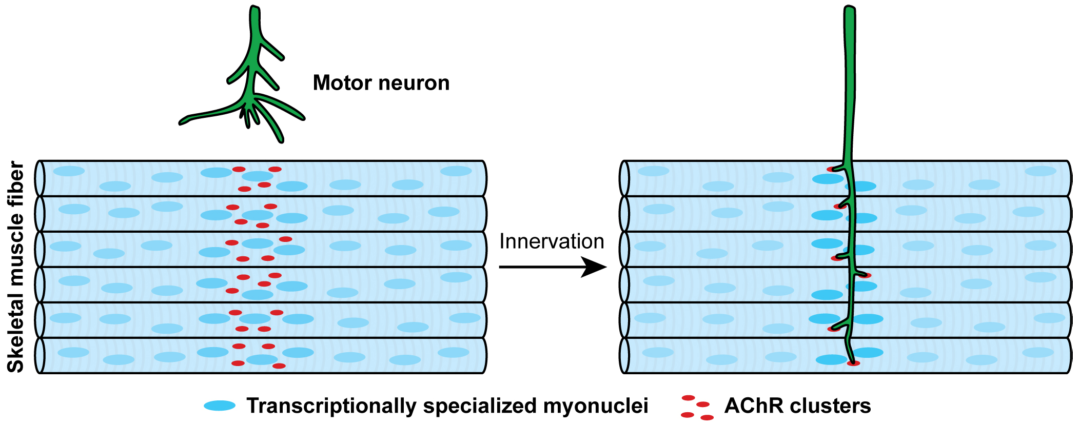
\includegraphics[width=\textwidth]{./Images/formation_jnm.png}
		\caption{Formation de la \gls{jnm}.} 
		\descfig{Figure issue de Burden \emph{et al.} 2018 \cite{Burden2018}.}
		\label{fig:FormaJNM}
	\end{figure}
	
	\todo{mettre avec section musk ?}
	Cette accumulation de \glspl{achr} lors du pré-patterning de la jonction, comme d'un certain nombre de protéines synaptiques, est due à un récepteur particulier : \gls{musk}. Ce dernier joue un rôle clef dans la formation de la synapse, sa position déterminant la position de cette dernière \cite{DeChiara1996, Glass1996}.
	
\section{Le récépteur \acrshort{musk}, une molécule clef de la synaptogénèse}
\label{sec:IntroMuSK}	
	\begin{wrapfigure}{l}{0.25\textwidth}
		\centering{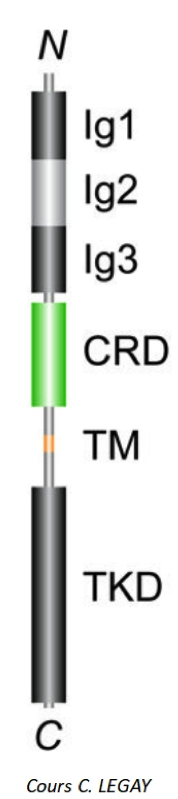
\includegraphics[width=0.1\textwidth]{./Images/MuSKReceptor.png}}
		\caption{Récepteur \gls{musk}}
		\descfig{Ig : Domaine immunoglobuline, CRD : \emph{Cysteine Rich Domain}, TM : Domaine transmembranaire,TKD : Domaine tyrosine kinase.}
		\label{fig:RMuSK}
	\end{wrapfigure}
	
	\acrfull{musk} est un récepteur découvert dans l'organe électrique de la raie \emph{Torpedo california} \cite{Jennings1993}. L'expression de ce récepteur à d'abord été mesurée dans les cellules musculaires et localisée au niveau de la \gls{jnm}. \gls{musk} est une récepteur tyrosine-kinase de 98kDa, dans lequel on distingue trois parties : un ectodomaine (partie N-terminale), un domaine transmembranaire, et un domaine cytoplasmique qui porte l'activité kinasique (voir \cref{fig:RMuSK}). 
	
	La partie extracellulaire comporte généralement trois domaines \gls{ig}, dont le domaine \gls{ig}1 a récemment été impliqué dans la liaison avec \gls{lrp}4 \cite{Zhang2011}, ainsi qu'un domaine Frizzled-like, riche en cystéines (\gls{crd}) \cite{Jing2009}.
	
	\gls{musk} possède trois ligands connus : l'Agrine (via \acrshort{lrp}4), un collagène spécifique associé à l'\Gls{ache} appelé \acrshort{colq}, et les \Glspl{wnt}, tous nécessaire au développement complet de la synapse. Un défaut de signalisation de l'un d'entre eux entraîne ainsi des défauts structuraux et/ou fonctionnels de la synapse.
	
	%Précédemment à la fin de section 1.
	L'Agrine est le ligand historique de \gls{musk} \cite{Glass1996}, et est sécrété par l'axone au contact de la cellule musculaire. Plus récemment, des travaux ont montré que l'Agrine se fixait en fait sur le co-récépteur de \gls{musk} : \gls{lrp}4 \cite{Zhang2008,Kim2008}. Suite à l'activation par l'Agrine de \acrshort{lrp}4, deux complexes \gls{musk}/\gls{lrp}4 vont s'assembler, et cet assemblage tétramérique permettrait une phosphorylation optimale de \gls{musk}, et donc une différenciation complète de la synapse et de l'agrégation des \gls{achr} \cite{Zong2012}.
	
	La présence de \gls{musk} dans le cerveau a longtemps été ignorée, du fait de sa faible expression dans cette organe, quantifiée dans le passé par Northern Blot, une méthode de détection des \acrshort{arnm} peu sensible. Cependant, de nouvelles techniques, telle que l'\gls{his} ou bien la \gls{qpcr}, ont permis de montrer que le récepteur était bien présent dans le tissu cérébral, principalement au niveau des neurones du cortex, du cervelet, et de l'hippocampe \cite{Garcia-Osta2006, Ksiazek2007}. Le récepteur \gls{musk} semble aussi être exprimé fortement dans les astrocytes \cite{Sun2016}, à des taux jusqu'à 5 fois supérieur à son expression dans les muscles squelettiques, où avec son co-récepteur \gls{lrp}4 il régulerait la transmission glutamatergiques au travers du relargage d'ATP et une signalisation liée à l'agrine.
	
	Au niveau du \gls{snc}, deux isoformes de \gls{musk} semblent être exprimées \cite{Garcia-Osta2006}. La première isoforme, de 2644pbs, est identique à une isoforme générée par épissage alternatif dans le muscle \cite{Valenzuela1995}, sans qu'aucun rôle ne lui soit connu pour l'instant. La seconde isoforme est plus courte : 2359pbs, et présente une délétion du troisième domaine \gls{ig}. Les deux isoformes présentent une alanine à la position 454 qui remplace une délétion de 8 acides aminé de l'éctodomaine. Une autre isoforme ayant le domaine \gls{ig}3 supprimé serait impliquée dans l'agrégation des \gls{achr} \cite{Hesser1999}.
	
	Grâce à des techniques de knockdown du gène par séquence antisens au niveau de l'hippocampe, il apparaîtrait que la présence de \gls{musk} dans le cerveau serait nécessaire mais non indispensable à la formation de la mémoire à moyen et long-terme \cite{Garcia-Osta2006}. La voie \gls{creb} est une voie impliquée dans la formation de la mémoire au niveau de l'hippocampe \cite{Silva1998, Kandel2012,Kida2014,Ortega-Martinez2015}, qui passerait par la phosphorylation de \gls{creb} suite au relargage de \acrshort{camp}, augmentant son activité transcriptionnelle. Un modèle propose \cite{Garcia-Osta2006} que l'activation de \gls{musk} activerait la cascade de signalisation de \gls{creb}, permettant la consolidation de la mémoire. Ce modèle expliquerait également l'auto-régulation de \gls{musk} \cite{Moore2001}, dont le gène possède dans sa séquence promotrice un élément CRE-like liant \gls{creb} \cite{Kim2005}. De plus, \gls{musk} est nécessaire à la formation de la \gls{ltp} de l'hippocampe \cite{Garcia-Osta2006}.

	Ainsi, le récepteur \gls{musk} possède comme ligand les protéines \glspl{wnt}. Ces protéines, connues pour leurs rôles prépondérant lors de la neurogénèse et de la mise en place des différentes structures du cerveau, semblent avoir un rôle important dans la mise en place de la jonction neuromusculaire, de concert avec \gls{musk}.

\section{Les protéines \Acrshortpl{wnt}, ligands de \acrshort{musk}}
\label{sec:IntroWnt}	
	\begin{wrapfigure}{l}{0.4\textwidth}
		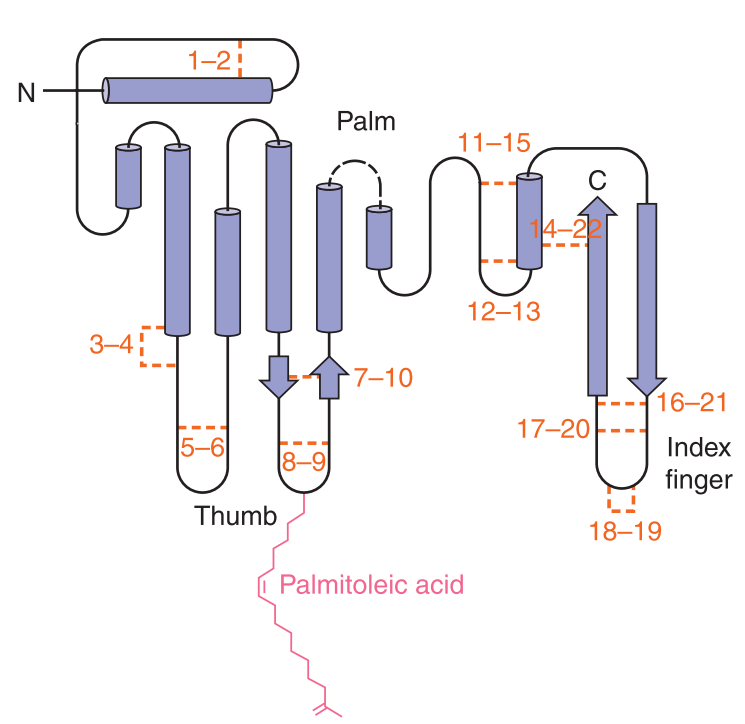
\includegraphics[width=0.4\textwidth]{./Images/WntProtein.png}	
		\caption{Structure d'une protéine \Gls{wnt} classique.}
		\descfig{Figure issue de Willert \& Nusse 2012 \cite{Willert2012}. En orange sont représentés les 22 résidus cystéines.}
		\label{fig:WntProt}
	\end{wrapfigure}
	
	Les \Acrfullpl{wnt} sont des glycoprotéines sécrétées, de 40kDa pour 350 acides aminés, impliquées dans de nombreux processus développementaux tel que l'embryogenèse, la prolifération, la différenciation, la migration cellulaire, ou encore l'apoptose \cite{Miller2002, Willert2012}. De plus, des travaux ont pu montrer que les \Glspl{wnt} étaient également impliquées dans des étapes précoces de la formation de la \gls{jnm} \cite{Hall2000}. En plus de leurs rôles durant le développement, les \Glspl{wnt} jouent également un rôle à l'age adulte dans la maintenance des tissus adultes. 
	
	La structure des \Glspl{wnt} est complexe, avec  de nombreux ponts disulfures caractéristiques de cette famille de protéines, d'hélices \textalpha{}, ainsi que la présence d'un acide palmitoléïque en Ser209 \cite{Takada2006} participant à la liaison avec le récepteur (voir \cref{fig:WntProt}). On peut également observer la présence d'un acide palmitique en position Cys77 \cite{Takada2006} conservé au cours de l'évolution. La présence de ces acides gras rendent les protéines \Gls{wnt} très hydrophobes, ce qui a retardé leurs caractérisations.
	
	On connaît actuellement 19 membres de cette famille de protéine chez la souris et chez l'humain. Classiquement, les \Glspl{wnt} se lient sur le domaine \gls{crd} de leur récepteur canonique \gls{fz}, associé aux co-récepteurs \gls{lrp}5 ou 6, mais il existe d'autres récepteurs non canoniques tels que : \gls{ror} \cite{Cadigan2006, Gordon2006, Green2008}, \gls{ryk} \cite{Bovolenta2006, Fradkin2010}, ou bien encore \gls{musk} \cite{Jing2009}, qui possèdent également un \gls{crd}.
		
	Les protéines \gls{wnt} peuvent activer plusieurs voies de signalisation différentes dans la cellule :  la voie canonique/\textbeta{}-catenin, la voie \gls{pcp}, et d'autres voies indépendante de la \textbeta{}-catenin. Pour la voie canonique, en l'absence de \Glspl{wnt} sur le récepteur \gls{fz}, la \textbeta{}-catenin est continuellement marquée par le complexe \acrshort{gsk3}-\acrshort{apc}-\acrshort{ck1}. Ce complexe va phosphorylé la \textbeta{}-catenin, permettant sa reconnaissance par la \gls{btrcp}, une E3 ubiquitine-ligase, et son marquage pour destruction par le protéasome. Quand les \Glspl{wnt} se lient à \gls{fz}, \emph{Dishevelled} (une protéine centrale dans les différentes voie \glspl{wnt} \cite{Gao2010}) est recrutée à la membrane, permettant l'interaction de \gls{lrp}5/6 avec la \gls{gsk3}. Cette interaction va libéré la \textbeta{}-catenin qui s'accumule dans le cytoplasme, puis se translocalise dans le noyau, d'où elle va avoir un effet sur la transcription des gènes. 
	
	La voie \gls{pcp} est impliquée principalement dans la migration, la polarisation ainsi que le destin cellulaire. Cette voie dans le \gls{snc} est essentielle pour la gastrulation et la formation du tube neural durant l'embryogenèse \cite{Adler2002, Nejsum2009}. L'étude de la voie \gls{pcp} est complexe, car de nombreux acteurs de cette voie sont également impliqués dans d'autres voies de signalisations importantes. Les \Glspl{wnt} en se liant à \gls{fz} vont recrutés \emph{Dishevelled} à la membrane, conduisant à l'activation de \acrshort{rhoa} et \gls{rock}. L'activation de ces protéines va entrainé le remodelage du cytosquelette d'actine et du réseau microtubulaire, nécessaire à la morphogénèse cellulaire. La voie \gls{pcp} active également \acrshort{jnk} et c-JUN activant la transcription de gènes cibles \cite{Niehrs2012}.
	
	Enfin, parmi les voies \glspl{wnt} non canonique, la plus connue est la voie \Gls{wnt}/Calcium, ou \emph{Dishevelled} va activer la \acrshort{plc}, résultant en une augmentation de la concentration intracellulaire d'\acrshort{ip3} et de \acrshort{dag}. L'\acrshort{ip3} provoque l'ouverture des canaux calciques du \gls{re}. Cette augmentation de calcium active la \acrshort{pkc} et la \acrshort{campk2}, qui agissent sur la transcription nucléaires au travers de différents facteurs tels que \acrshort{creb} \cite{Koles2012}. Il est également a noté que dans certains cas, en réponse à une stimulation par \Gls{wnt}3, le récepteur \gls{ryk} était clivé par la \textgamma{}-sécrétase, induisant la translocation de la partie intracellulaire du récepteur dans le noyau \cite{Lyu2008}.
	
	\emph{In vitro}, il a été montrer que plusieurs \Glspl{wnt} interagissaient avec \gls{musk} : \Gls{wnt}2, 3a, 4, 6, 7b, 9a, et 11 \cite{Strochlic2012, Zhang2012, Barik2014}, avec différents effets. Seules \gls{wnt}4, 9a et 11 vont conduire à une dimérisation de \gls{musk} et à son activation (\emph{in vitro}). Ceci est cohérent avec le fait que chez le Poisson-zèbre, l'orthologue de \gls{musk}, \emph{unplugged}, possède aussi un \gls{crd} qui interagit avec des protéines \Glspl{wnt} pour induire l'agrégation de \glspl{achr} \cite{Jing2009, Gordon2012}. \Gls{lrp}4 semble être également nécessaire à l'agrégation des \gls{achr} médié par les \gls{wnt}s \cite{Zhang2012}.

\section{\acrshort{musk} et \Acrshortpl {wnt} : Contexte de l'étude et but du stage}
\label{sec:Contexte}	
	Dans le but d'étudier le rôle de l'interaction des protéines \Glspl{wnt} et du domaine \gls{crd} de \gls{musk}, l'équipe de C. LEGAY à crée une souris transgénique dont le \gls{crd} était supprimé (\mcrd) \cite{Messeant2015, Messeant2017}. Il a ainsi été montré que le \gls{crd} était nécessaire à la \gls{jnm} à la fois pour sa formation et pour son maintien à l'age adulte, et que \Gls{wnt}4 et 11 participaient activement à la formation de cette dernière. De plus, un traitement au \gls{licl} (inhibiteur de la \gls{gsk3}) permettait à la \gls{jnm} un retour vers un phénotype sauvage. 
	
	En plus de leurs problèmes musculaires, les souris \mcrd exhibaient des défauts centraux : durant son stage, une étudiante, Bertille SOMON, a montré que les mutants mâles avaient des blessures importantes au niveau du dos, blessures qui n'étaient pas dues à des comportements d'agressivité entre souris. De plus, une analyse comportementale a été réalisée en collaboration avec le groupe du Dr LANFUMEY (Centre de Psychiatrie et Neurosciences, Paris), et le test \gls{nor} a révélé que les souris mutantes souffraient d'un déficit de la mémoire intermédiaire.
	
	Comme \gls{musk} est exprimé dans le cerveau adulte, principalement au niveau de l'hippocampe \cite{Garcia-Osta2006}, et que ce lieu joue un rôle prépondérant dans la formation de la mémoire intermédiaire, l'objectif de mon stage va être d'explorer le rôle de l'interaction de \gls{musk} et des \Glspl{wnt} dans le cerveau, utilisant pour cela les souris \mcrd. Je poserai au cours de mon stages plusieurs questions : Quelle est l'origine des blessures observées chez le mâle, est-ce que la structure du cerveau est affectées chez le mutant, quelles sont les cellules exprimant \gls{musk}, et quel est le niveau d'expression du gène dans différentes structures du cerveau.

%Cela se fera au travers de 5 axes : 
%\begin{enumerate}
%	\item \sout{Quelle est l'origine des blessures chez le mâle ?}
%	\item La structure du cerveau est-elle affectée chez le mutant ?
%	\item Quelles sont les cellules exprimant \gls{musk} ?
%	\item Quel est le niveau d'expression de \gls{musk}/\mcrd dans le cerveau ?
%	\item \sout{Un traitement au \gls{licl} peut-il permettre un retour du mutant à un phénotype sauvage au niveau du comportement ?}
%\end{enumerate}
\FloatBarrier %Empeche figures etc d'aller dans chap. suivants

\chapter{Matériels et Méthodes}
 % !tex root= main.tex
\paragraph{Animaux et Prélèvements}
\label{par:AnimEtPrelev}
	Les souris utilisées sont issues d'une lignée hétérozygote provenant d'un fond génétique mixte \cite{Messeant2015, Messeant2017}. Les souris mutantes \mcrd et \gls{wt} testées sont issues de même portée. Afin de prélever les cerveaux, les souris sont  euthanasiées à l'aide d'une injection intrapéritonéale de Pentobarbital (Ceva\textregistered) à une dose de 40µg/mg. Une perfusion péristaltique de \gls{pfa} 4\% est réalisée pour fixer les tissus. Le cerveau est prélevé et post-fixé dans du \gls{pfa} 4\% pendant 1 heure, puis transféré dans une solution de sucrose 30\% à 4°C jusqu'à utilisation. 
	
\paragraph{Génotypage}
\label{par:genotypage}
	Les animaux sont génotypés à l'âge de 7 jours par prélèvement d'un doigt d'une patte antérieure. L'extraction d'\acrshort{adn} se fait par lyse alcaline (NaOH 25mM, 95°C, 20 minutes) puis ajout de Tris-HCl 40mM pour arrêter la réaction. Une \acrshort{pcr} est réalisée avec les couples de primers Ef et Lxr  pour les individus \gls{wt}, et Ef et Wr pour les individus mutant (voir \cref{table:génotypage} pour les séquences des primers utilisés). Dépôt des produits de \acrshort{pcr} dans un gel d'agarose 2\% - \acrshort{bet}, migration à 200V pendant 10 minutes et révélations des bandes aux ultraviolets.
	
	\begin{table}[h]
		\centering{
			\begin{threeparttable}
				\caption{Séquence des primers utilisés pour le génotypage}
				\label{table:génotypage}
				\begin{tabular}{|c || c|}
					\hline
					Primers 						& Séquence \\
					\hline
					Ef 								& 5'-CTC TTC TCC CTT CTG CCC ACC GAT-3' \\
					\hline
					Lxr								& 5'-AGT TAT ACT AGA GCG GCC GTT CAC CG-3'\\
					\hline
					Wr								& 5'-CCC TGG GAA TAT GGT TTC TCA TTG CT-3' \\
					\hline	
				\end{tabular}
			\end{threeparttable}
		}
	\end{table}
\FloatBarrier
	
\paragraph{Real-Time \acrshort{rtpcr} (\acrshort{qpcr})}
\label{par:qPCR}
	Les hippocampes droits et gauches ont été disséqués et immédiatement plongés dans 800µl de TRIzol\textregistered, broyés mécaniquement avec un TissuRuptor II (Qiagen\textregistered) puis stockés à -20°C. L'extraction de l'\acrshort{arn} a été faite sur colonne grâce au RNeasy Protect Mini Kit (Qiagen\textregistered). Le traitement à la DNAse puis la transcription inverse des ARN suivie d'une PCR (\acrshort{rtpcr}) ont été réalisées avec le RT\up{2} First Strand Kit (Qiagen\textregistered). La \gls{qpcr} est faite avec du SYBR Green/ROX qPCR Master Mix (ThermoFisher\textregistered) contenant une Taq Polymerase et des \glspl{dntp}. Les primers utilisés (fournis et testés par Qiagen\textregistered) sont dirigés contre \gls{musk} et \acrshort{26s} (sous-unité du protéasome, gène de ménage couramment utilisé chez la souris).
	
\paragraph{Coloration de Nissl}
\label{par:Nissl}
	Des coupes de cerveaux de 50µm sont réalisées au microtome à partir du cerveau de 4 souris : 1 femelle mutante, 1 mâle mutant, 1 femelle sauvage et 1 mâle sauvage. Une coupe sur 3 est séléctionnée puis montée sur lame avec de la gélatine de porc 1\%. Après séchage à l'air libre pendant 24 heures, les lames sont déshydratées et dégraissées dans des bains successifs d'éthanol 70°, 95°, 100° et de xylène. Les lames sont ensuite réhydratées dans des bains d'éthanol de concentrations décroissantes puis d'eau déminéralisée avant d'être plongées dans le colorant de Nissl (solution de Crésyl Violet).  Les lames sont rinçées dans de l'eau déminéralisée puis à nouveau déshydratées et immergées dans un bain de xylène. Le montage des coupes est fait dans du milieu Eukitt\textregistered (Sigma).
	
\paragraph{\Acrlong{ihc} sur coupes}	
\label{par:ihccoupe}
	Pour l'\Gls{ihc}, des coupes de 40µm sont réalisées au cryostat, et récupérés dans des puits contenant du \acrshort{pbs}. Lors du marquage, les coupes sont incubées 1 heure à température ambiante dans un sérum de blocage (\acrshort{pbs}, Sérum de chèvre 5\%, \acrshort{bsa} 3\%, Triton X-100 2\%), puis  incubées dans 500µl de solution d'incubation (\acrshort{pbs}, \acrshort{bsa} 3\%, Triton X-100 0.5\%) avec les anticorps pendant une nuit à 4°C avec agitation. Le lendemain, les coupes sont rinçées dans la solution de blocage diluée, incubées 2 heures avec l'anticorps secondaire dans le noir à température ambiante, puis 20 secondes avec du \gls{dapi}. Les lames sont à nouveau rinçées dans la solution précédente, et sont montées dans du milieu de montage Mowiol ou FluoroMount-G\textregistered.
	
\paragraph{\Acrlong{ihc} sur cultures cellulaires}
\label{par:ihcculture}
	Des cultures primaires de neurones et d'astrocytes provenant d'hippocampes de souris sont fixés dans un mélange \gls{pfa}4\%-Sucrose 4\% avant d'être stockées à 4°C dans du \gls{pfa} 0.4\%. Les cultures sont rincées au \acrshort{pbs}, incubées 10 minutes dans du Triton 0.5\%, à nouveau rinçées au \acrshort{pbs}, puis incubées avec du sérum de blocage (\acrshort{bsa} 3\%, Sérum de chèvre 5\%) 2 heures à température. Les anticorps primaires dilués dans la solution de blocage sont ajouté pour une incubation à 4°C sur la nuit.  Après rinçage au \acrshort{pbs}, les cultures cellulaires sont incubées avec l'anticorps secondaire, puis du \acrshort{dapi} et enfin montées.
	
\paragraph{Mesures de l'hippocampe}
\label{par:hippNeuN}
	Après marquage des neurones contre \acrshort{neun}, trois mesures sont effectuées sur trois coupes par cerveau dans diverses régions des hippocampes droit et gauche : CA1, CA3, Partie interne et externe du Gyrus Denté ainsi que son extrémité. Les trois coupes sont choisies dans le sens antéro-postérieur pour représenter le développement 3D de la structure. Les mesures mutantes versus sauvages sont alors comparées régions par régions.
	
\paragraph{Lyse des tissus}
\label{par:lyse}
	Les tissus disséqués sont immédiatement congelés par immersion dans de l'azote liquide, puis stockés à -80°C. Ceux-ci sont ensuite rassemblés avant d'être plongés dans du tampon RIPA (10mL de tampon par gramme d'échantillons) additionné d'un cocktail d'inhibiteur de protéases (1:25). Les échantillons sont ensuite broyés mécaniquement avec un TissuRuptor II (Qiagen\textregistered) puis incubés sur de la glace pendant 1 heure avec agitation. Après une centrifugation à $20\,000G$, 4°C pendant 15min, le surnageant est récupéré et stockés à -20°C. 
	
\paragraph{\Acrlong{ip}}
\label{par:ip}
	Le dosage des protéines est effectué par BC Assay. L'équivalent de 3mg de protéines est dilué dans 500µL de tampon RIPA auquel est ajouté 5µL d'anticorps (non dilué), puis incubé sur la nuit, 4°C avec mélange. Des billes magnétiques (Dynabead\textregistered Protein G) sont lavées puis mise en incubation avec la solution antigène-anticorps 3 heures à 4°C avec mélange. Le surnageant est récupéré et mis de coté comme contrôle. Les billes sont lavées dans du tampon RIPA, puis avec du tampon Tris 50mM. La séparation des protéines et des billes est réalisées en ajoutant du Bleu de Laemmli 1X chauffés à 70°C 10 minutes. Le surnageant est récupéré et stocké à -20°C. 
	
\paragraph{\Acrlong{wb}}
\label{par:wb}
	Les échantillons sont migrés sur un gel Mini-PROTEAN\textregistered{}  TGX 10\% à 80V pendant 10 minutes puis 120V dans du tampon Tris/Glycine/SDS pour ensuite être transférés sur une membrane de nitrocellulose sur la nuit à 4°C, 40V, avec du tampon Tris/Glycine. La membrane est ensuite colorée au Rouge Ponceau afin de vérifier la présence de protéines, décoloré par lavage dans du \acrshort{pbst}, mise 2 heures avec agitation dans du tampon de blocage (Pierce™ Protein-Free (PBS) Blocking Buffer) puis incubés avec l'anticorps primaire dilué dans le tampon de blocage une nuit à 4°C avec agitation. La membrane est lavée dans du \acrshort{pbst} puis incubée avec l'anticorps secondaire (dilué dans du tampon de blocage) 45 minutes. La révélation est faite par un kit Amersham\texttrademark ECL\texttrademark prime.
		
\paragraph{Anticorps}
\label{par:anticorps}
	Les anticorps utilisés pour l'\acrfull{ihc} et l'\acrfull{ip} sont présentés dans la \cref{table:Ac}.
	
	\begin{table}[h]
		\centering{
			\begin{threeparttable}
				\caption{Références des Anticorps utilisée et leurs dilution.}
				\label{table:Ac}
				\begin{tabular}{c | l l l l}
					\hline		
					& \teteCol{Anticorps} 	& \teteCol{Source} 	&\teteCol{Réf.}	& \teteCol{Dilution}\\
					\hline 
					%%% Immunomarquage
					\Acrshort{ihc}	&Rabbit @-\acrshort{musk}	&Millipore		&ABS549		&$1{:}500$ \\
									&Rabbit @-\acrshort{neun}	&Abcam			&ab105225	&$1{:}500$ \\
									&Mouse @-\acrshort{gfap}	&Millipore 		&MAB360		&$1{:}1\,000$ \\
									&Mouse @-\acrshort{gfap}    &Abcam			&ab4648     &N/A\\
									&Guinea Pig @-\acrshort{glt1} &Millipore	&AB1783		&$1{:}5\,000$\\
									&Goat @-Rabbit-A488			&Invitrogen		&A11008		&$1{:}500$\\
									&Goat @-Mouse-A594			&Invitrogen 	&A11005		&$1{:}500$\\
					\hline
					%%% Immunoprécipitation
					\Acrshort{ip} 		&Rabbit @-\acrshort{musk} 	&Millipore 	&ABS549	&$1{:}1\,000$\\
										&@-Rabbit-\acrshort{hrp}	&Amersham	&NA934	&$1{:}20\,000$\\
										&@-Light Chain Rabbit-\acrshort{hrp} & ???	& ???	&$1{ : }1\,000$\\
					\hline
				\end{tabular}
			\end{threeparttable}
		}
	\end{table} 
	\FloatBarrier
	
\paragraph{Acquisition d'images et Statistiques}
\label{par:ImagesStats}
	Les images ont été prises avec un microscope Epifluo Nikon Eclypse TE-2000E équipé d'une caméra Photometrics CoolSNAP HQ2 (Fluorescence) et d'une caméra Qimaging Color Retiga 2000R (Lumière blanche).
	Les images ont été traitées avec le logiciel ImageJ \cite{Schneider2012}.
\FloatBarrier %Empeche figures etc d'aller dans chap. suivants

\chapter{Résultats}
\section{Structure du cerveau}
\label{sec:NisslResultat}

	\subsection{Organisation globale du cerveau}
	\label{ssec:orgaglobale}
		La coloration de Nissl, ici à base de Crésyl violet, est un marquage classique du tissu nerveux avec une molécule basique, qui marque fortement l'acide nucléique (\acrshort{adn} et \acrshort{arn}) des cellules car basophile (ces structures au microscope prennent le nom de "Corps de Nissl'). Ce marquage est important dans les neurones, riches en \gls{re} rugueux, organite associé à une grande quantité d'\acrshort{arn}. Cette coloration permet ainsi de visualiser les différentes structures cellulaires au sein du tissu nerveux.
	
		Comme les protéines \gls{wnt} sont généralement impliquées dans le développement et l'organisation du cerveau, on peut alors se demander si la suppression du domaine de liaisons de ces protéines sur le récepteur \gls{musk} allait entraîner des modifications du développement du système nerveux qui serait visible avec une coloration histologique.
	
		Afin de comparer l'organisation structurale du cerveau chez la souris sauvage et mutante, une coloration de Nissl a donc été réalisée sur 4 individus : 2 souris mutantes et 2 souris sauvages (1 mâle et 1 femelle pour chaque groupe) (\cref{fig:NisslResultat}). Ce marquage a permis de mettre en évidence que la mutation de \gls{musk} ne modifiait pas l'organisation globale du cerveau, à la fois chez les souris femelles (\cref{fig:FemWTNissl,fig:FemMutNissl}) et mâles (\cref{fig:MaleWTNissl,fig:MaleMutNissl}). 
	
		\begin{figure}[h] %Figure Nissl Résultats
			\begin{center}
				\begin{subfigure}[h]{0.49\textwidth}%F437 WT Nissl 33 l2.tif
					\caption{}
					\label{fig:FemWTNissl}
					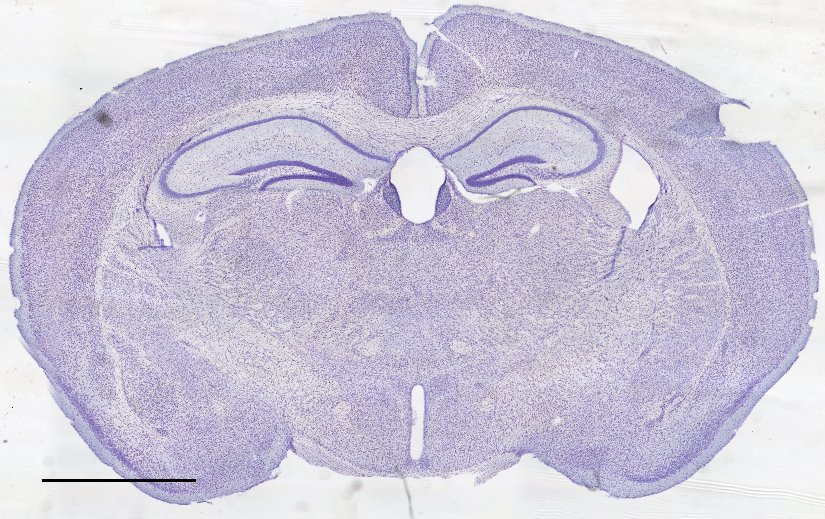
\includegraphics[width=\textwidth]{./Images/Nissl/FemWT.jpg}
				\end{subfigure}
				\begin{subfigure}[h]{0.49\textwidth}%F435 Mut Nissl 38.tif
					\caption{}
					\label{fig:FemMutNissl}
					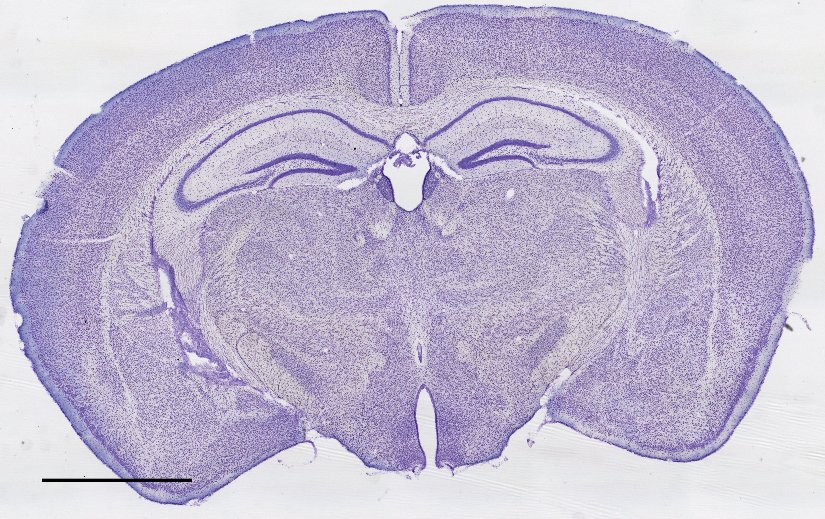
\includegraphics[width=\textwidth]{./Images/Nissl/FemMut.jpg}
				\end{subfigure}
				\begin{subfigure}[h]{0.49\textwidth}%M2 WT Nissl #031.tif
					\caption{}
					\label{fig:MaleWTNissl}
					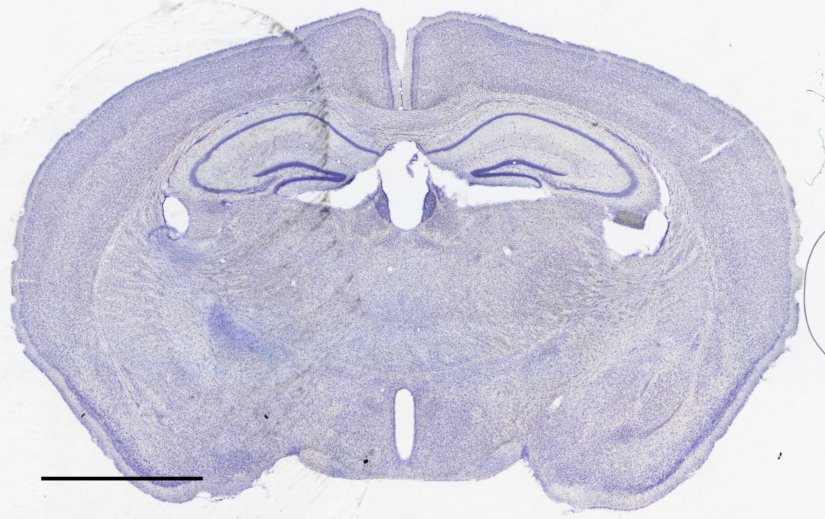
\includegraphics[width=\textwidth]{./Images/Nissl/MaleWT.jpg}
				\end{subfigure}
				\begin{subfigure}[h]{0.49\textwidth}%M442 Mut Nissl lame 3 36.tif
					\caption{}
					\label{fig:MaleMutNissl}
					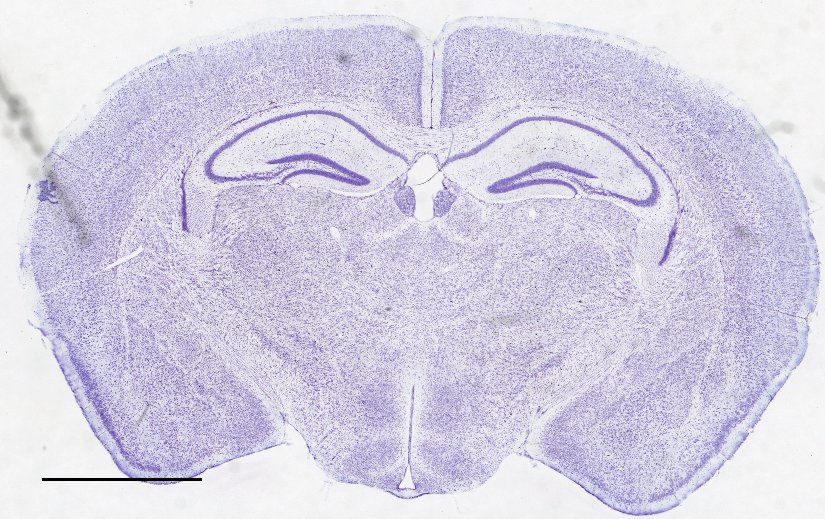
\includegraphics[width=\textwidth]{./Images/Nissl/MaleMut.jpg}
				\end{subfigure}
			\end{center}
			\caption{Les souris \mcrd ne présentent pas de défauts de structure globale du \acrshort{snc}.}
			\descfig{%
				Coloration de Nissl sur : 
				\subref{fig:FemWTNissl} Femelle sauvage, 
				\subref{fig:FemMutNissl} Femelle mutante, 
				\subref{fig:MaleWTNissl} Mâle sauvage, 
				\subref{fig:MaleMutNissl} Mâle mutant. 
				Images représentatives de coupes réalisées au niveau de l'hippocampe. 
				Âge moyen des souris : 30 jours. 
				Barre d'échelle : 2 mm.
				n = 4 (une souris de chaque sexe mutante ou sauvage).
					}
			\label{fig:NisslResultat}
		\end{figure}
		\FloatBarrier

	\subsection{Distribution des neurones dans l'hippocampe}
	\label{ssec:neun}
		Pour visualiser l'organisation des neurones dans l'hippocampe des souris mutantes, j'ai révélé les neurones par \acrshort{ihc} en utilisant des anticorps dirigés contre \acrshort{neun}. \Acrshort{neun} (connu aussi sous le nom de Fox-3) est un marqueur du  corps cellulaire et des noyaux de presque tous les neurones, couramment utilisé dans les études neurologiques \cite{Guselnikova2015, Kim2009}. 
		
		Grâce à des mesures d'épaisseur de la couche pyramidale (CA1, CA3) et granulaire (Gyrus Denté) réalisées dans différentes régions de l'hippocampe sur des coupes rostrale, médiane et caudale, il apparaît que la structure de l'hippocampe est modifiée chez les souris mutantes par rapport aux souris sauvages (\cref{fig:NeuNResultat}). En comparant les mesures des coupes rostrales, on observe une différence dans la région du Gyrus Denté (72.50$\pm$18.17µm (\acrshort{wt}) vs 57.30$\pm$13.84µm (mutant), p-value : 0.0138) (\cref{fig:NeunQuantifNasal}).  Au niveau de coupes médianes, aucune différences ne ressort des différentes mesures effectuées (\cref{fig:NeunQuantifMilieu}). Pour les coupes caudales, on peut observer une différences d'épaisseur de la couche entre les souris \gls{wt} et \mcrd dans la région CA3 (111.20$\pm$20.39µm (\acrshort{wt}) vs 78.39$\pm$39.22 (mutant), p-value : 0.0129), et les deux sous-région du Gyrus denté (DG1 : 50.29$\pm$9.655 (\acrshort{wt}) vs 63.44$\pm$17.37 (mutant), p-value : 0.0244 ; et DG2 : 61.29$\pm$10.24 (\acrshort{wt}) vs 51.78$\pm$12.46 (mutant), p-value : 0.0367)(\cref{fig:NeunQuantifPost}).
		
		\begin{figure}[h]
			\begin{subfigure}[h]{0.329\textwidth} %M2 WT NeuN 3.tiff
				\caption{}
				\label{fig:NeuNIllu1}
				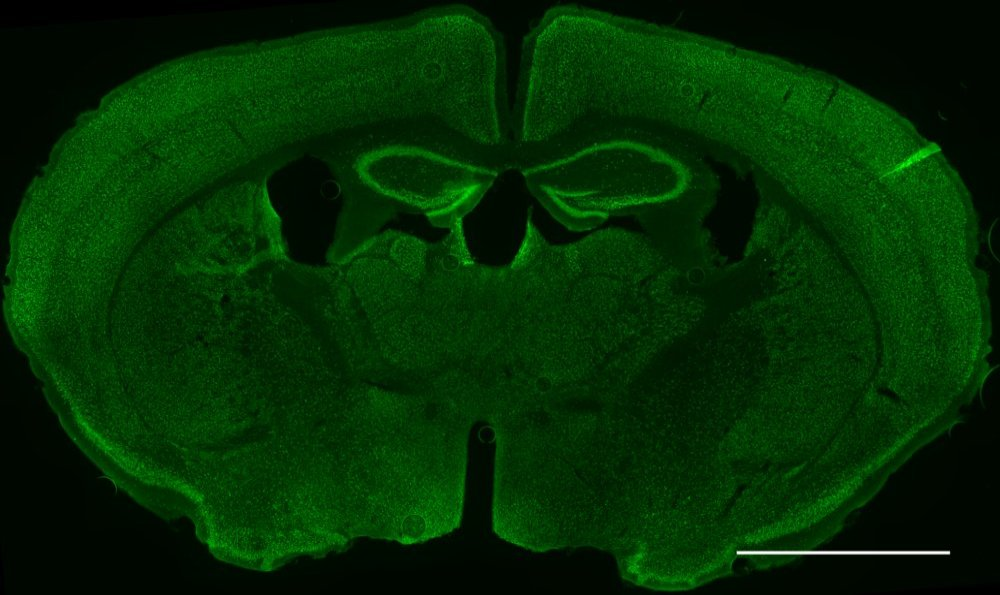
\includegraphics[width=\textwidth]{./Images/Immuno/NeuN/M2WT_NeuN_10x_1.jpg}
			\end{subfigure}
			\begin{subfigure}[h]{0.329\textwidth} %M2 WT NeuN 5.tiff
				\caption{}
				\label{fig:NeuNIllu2}
				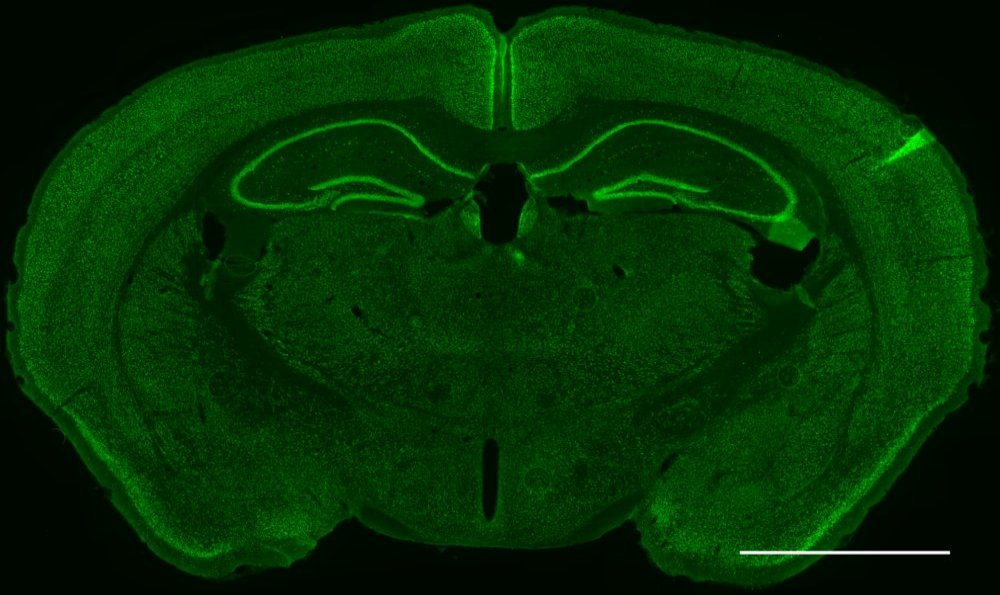
\includegraphics[width=\textwidth]{./Images/Immuno/NeuN/M2WT_NeuN_10x_2.jpg}
			\end{subfigure}
			\begin{subfigure}[h]{0.329\textwidth} %M2 WT NeuN 7.tiff
				\caption{}
				\label{fig:NeuNIllu3}
				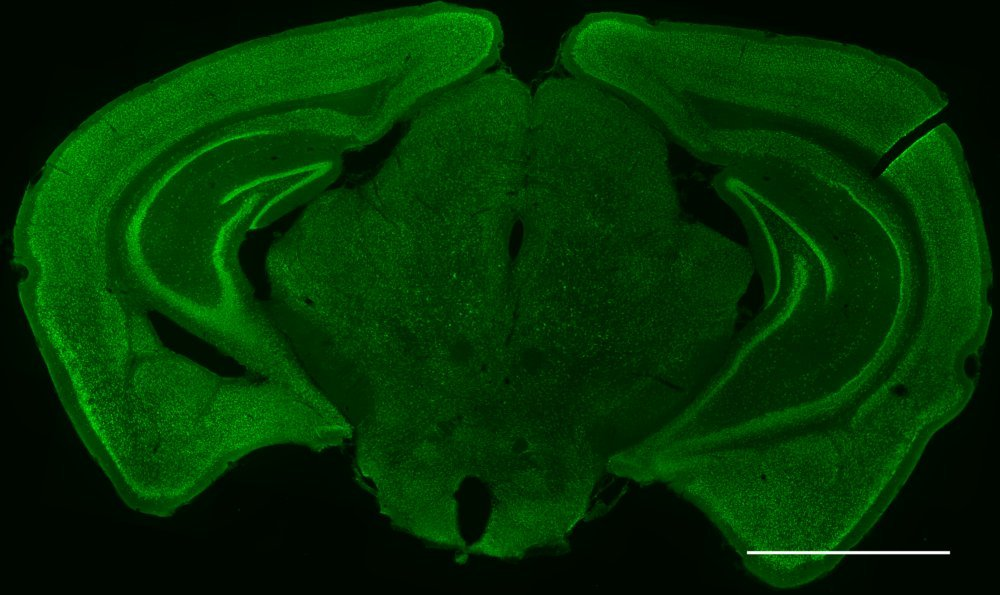
\includegraphics[width=\textwidth]{./Images/Immuno/NeuN/M2WT_NeuN_10x_3.jpg}
			\end{subfigure}
			\begin{subfigure}[h]{0.329\textwidth}
				\caption{}
				\label{fig:hippIllu}
				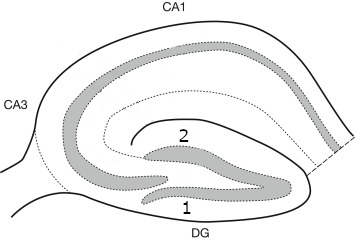
\includegraphics[width=\textwidth]{./Images/HippSchema.jpg}
			\end{subfigure}
			\begin{subfigure}[h]{0.329\textwidth}
				\caption{}
				\label{fig:NeunQuantifNasal}
				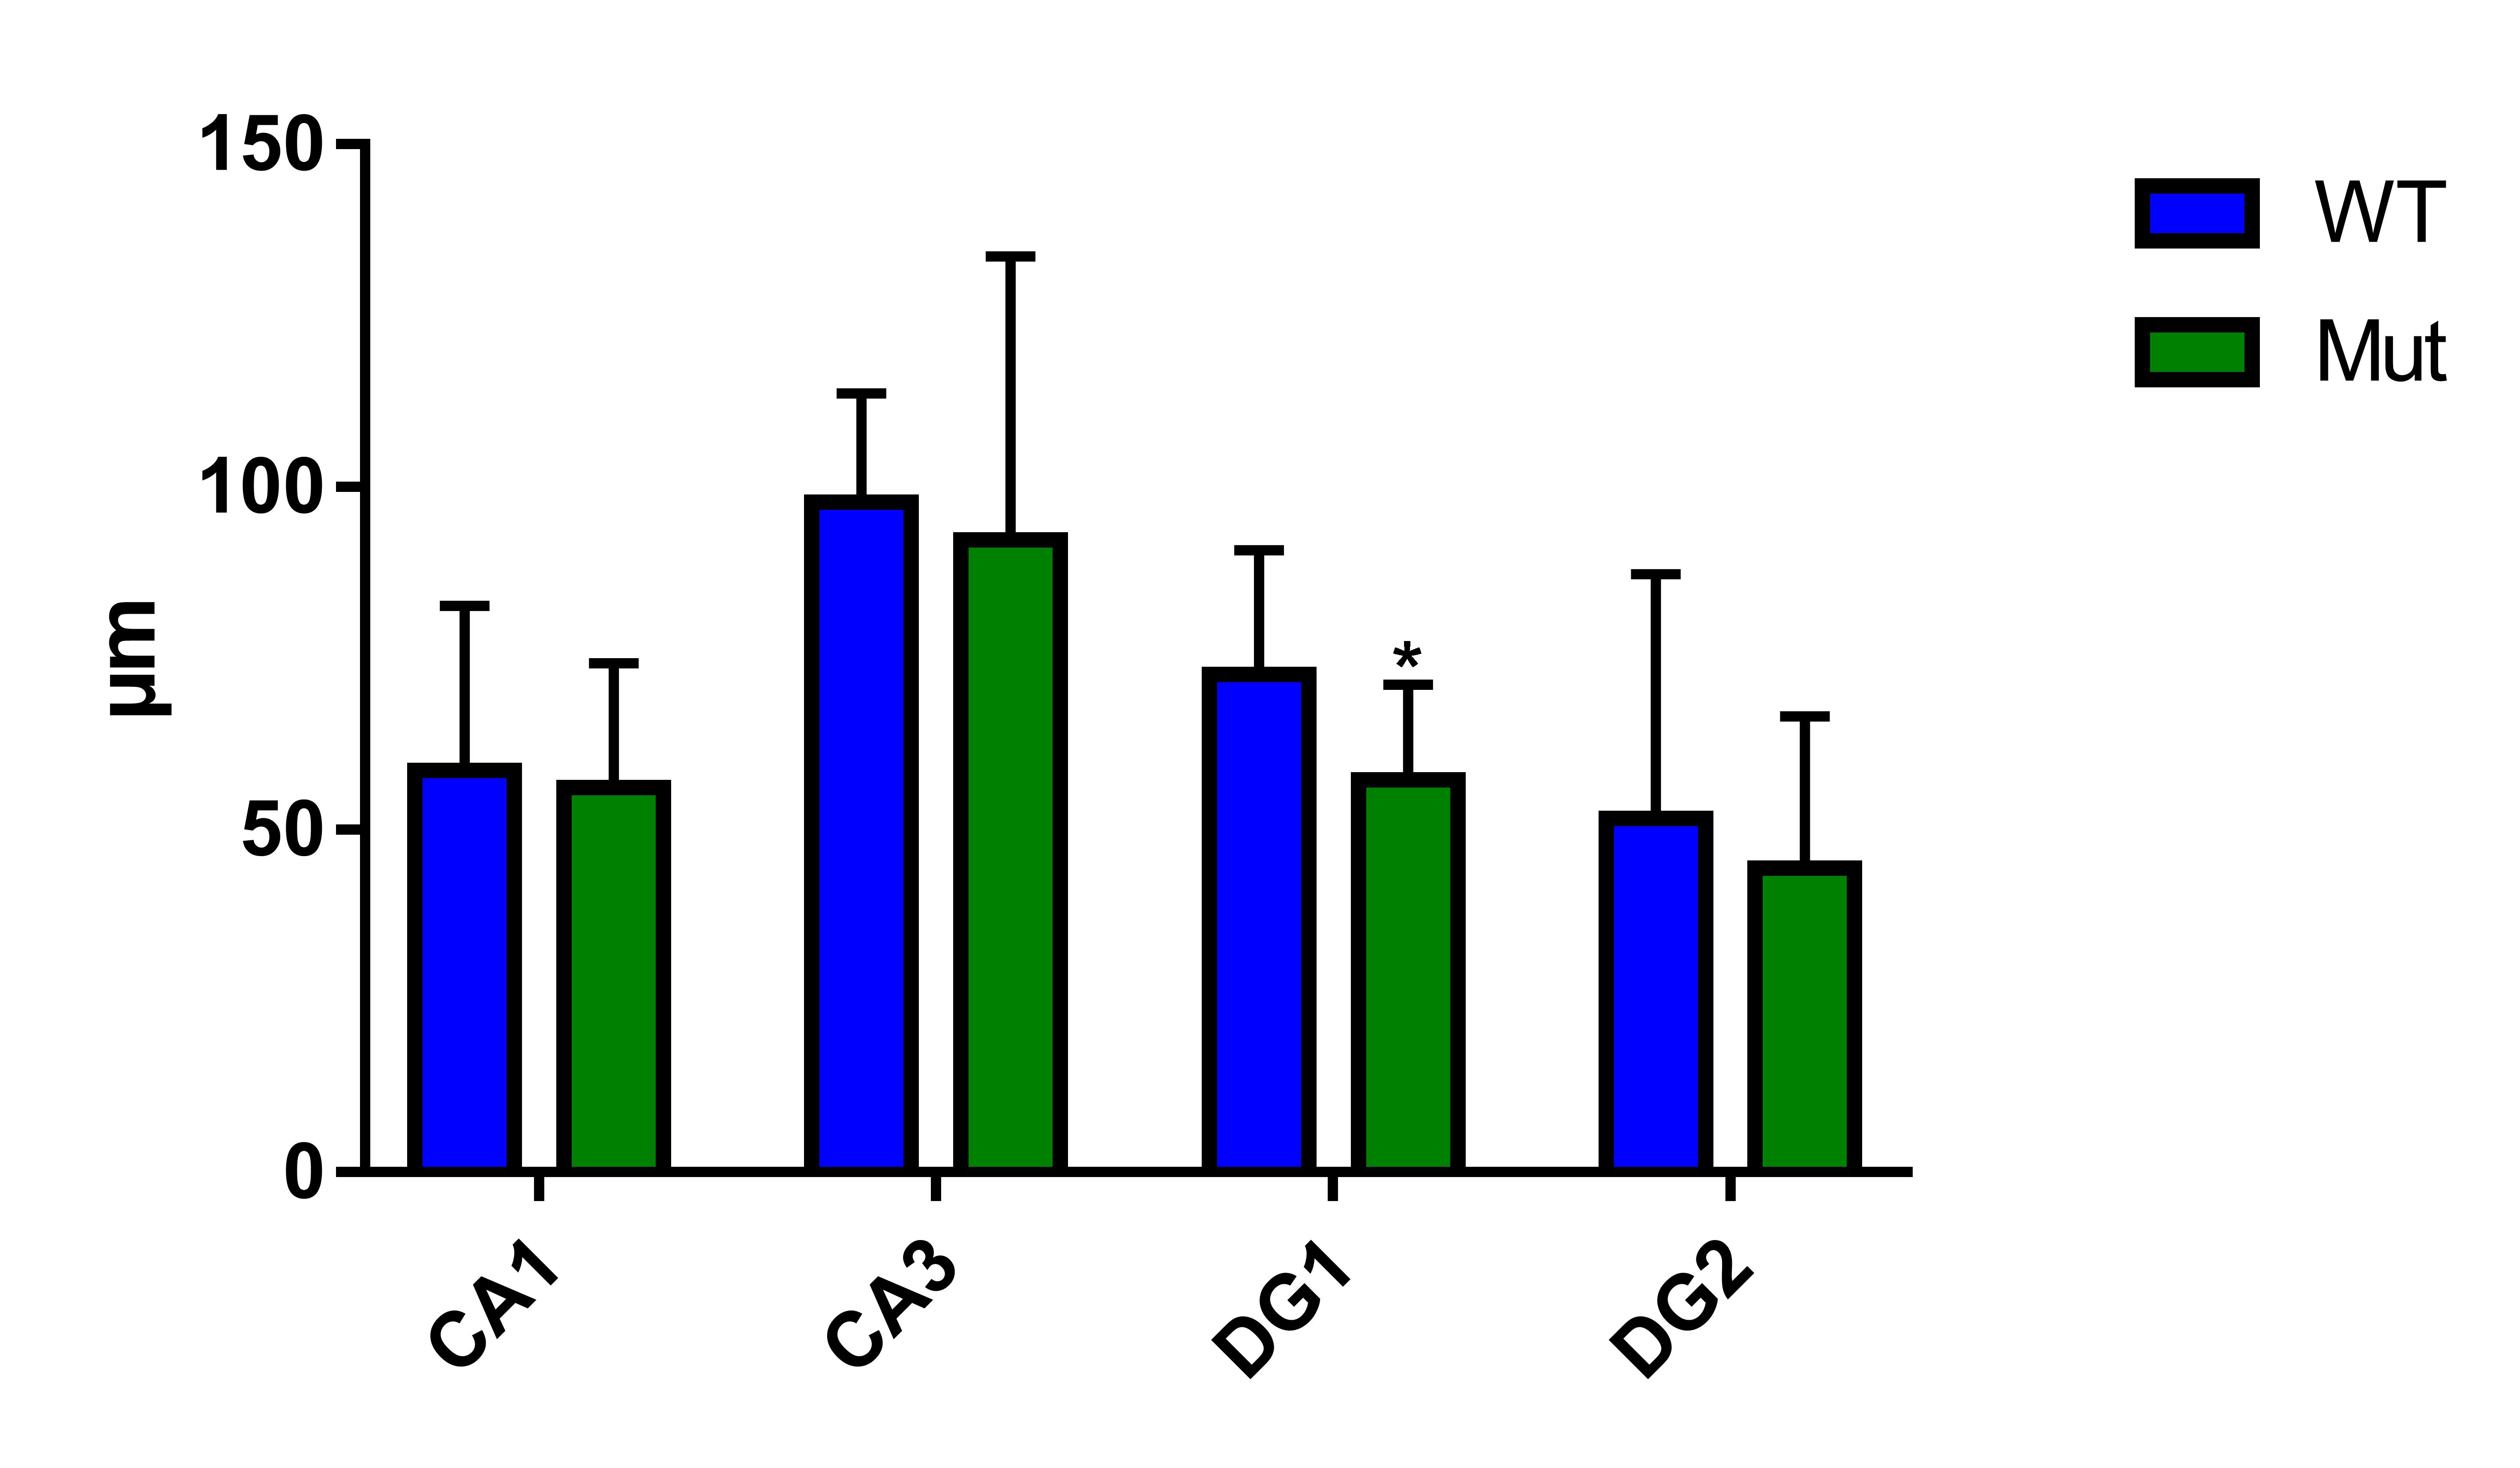
\includegraphics[width=\textwidth]{./Images/Immuno/NeuN/Quantif_Nasal.jpg}
			\end{subfigure}
			\begin{subfigure}[h]{0.329\textwidth}
				\caption{}
				\label{fig:NeunQuantifMilieu}
				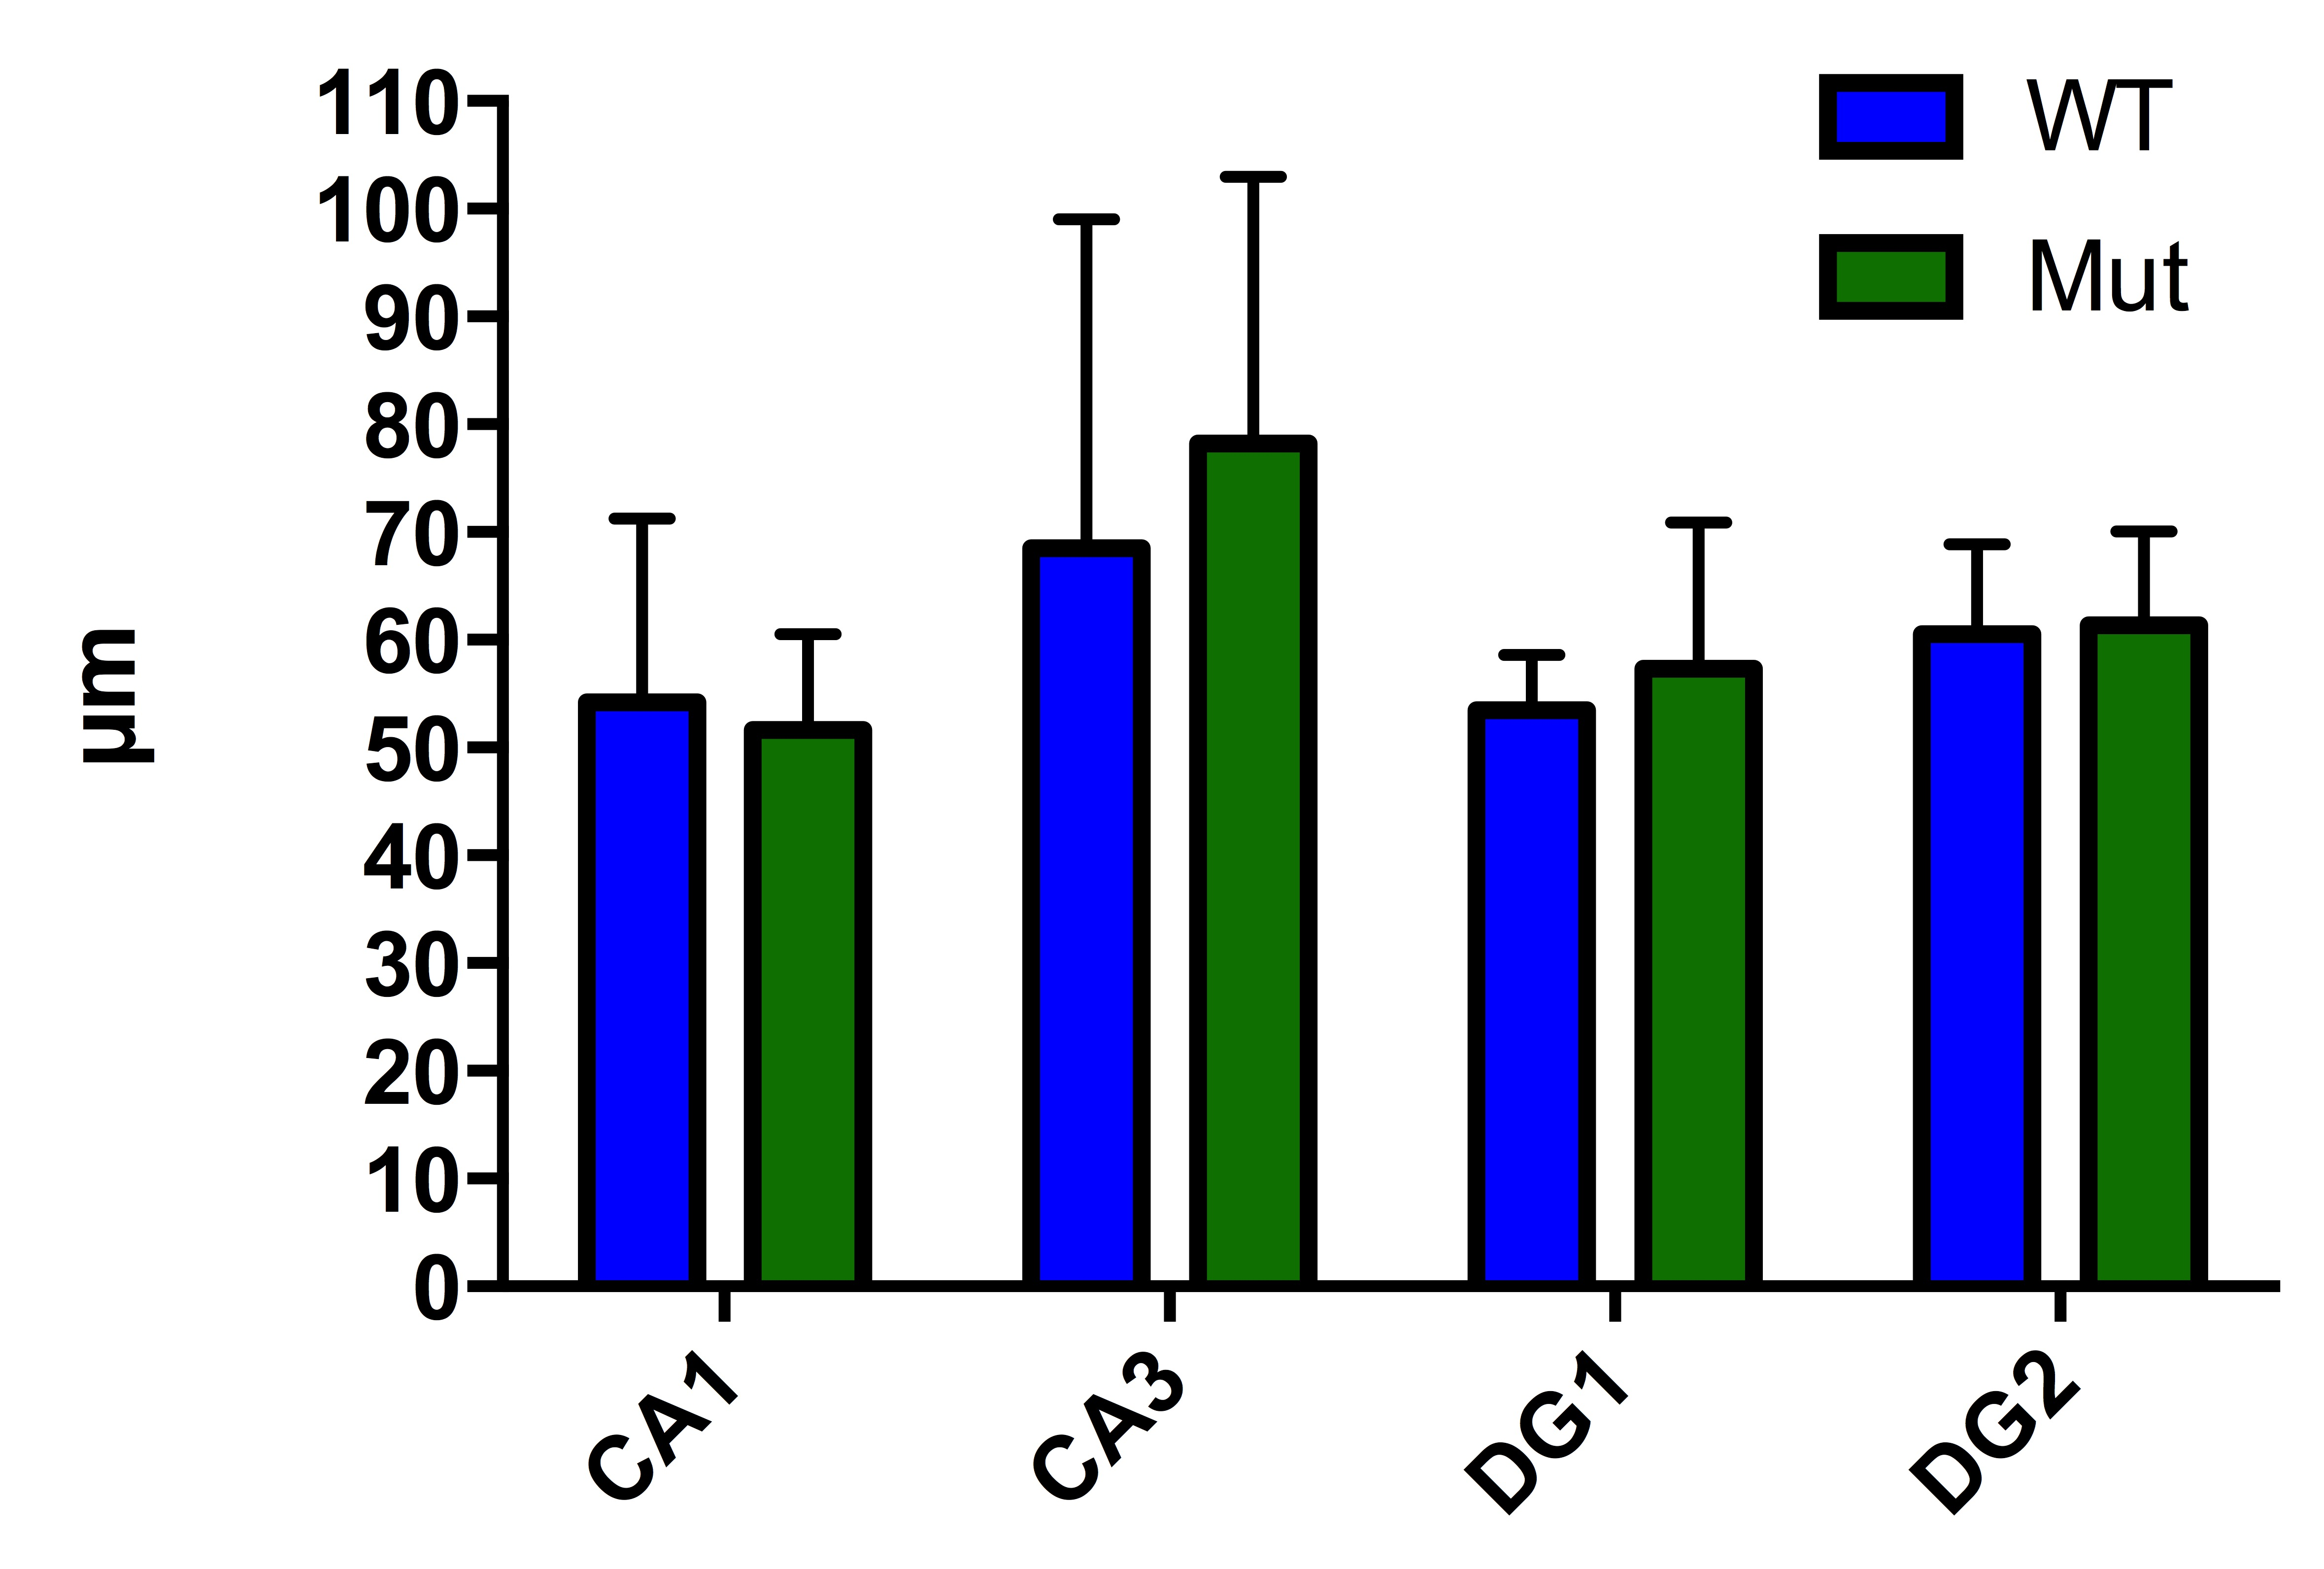
\includegraphics[width=\textwidth]{./Images/Immuno/NeuN/Quantif_Milieu.jpg}
			\end{subfigure}
			\begin{subfigure}[h]{0.329\textwidth}
				\caption{}
				\label{fig:NeunQuantifPost}
				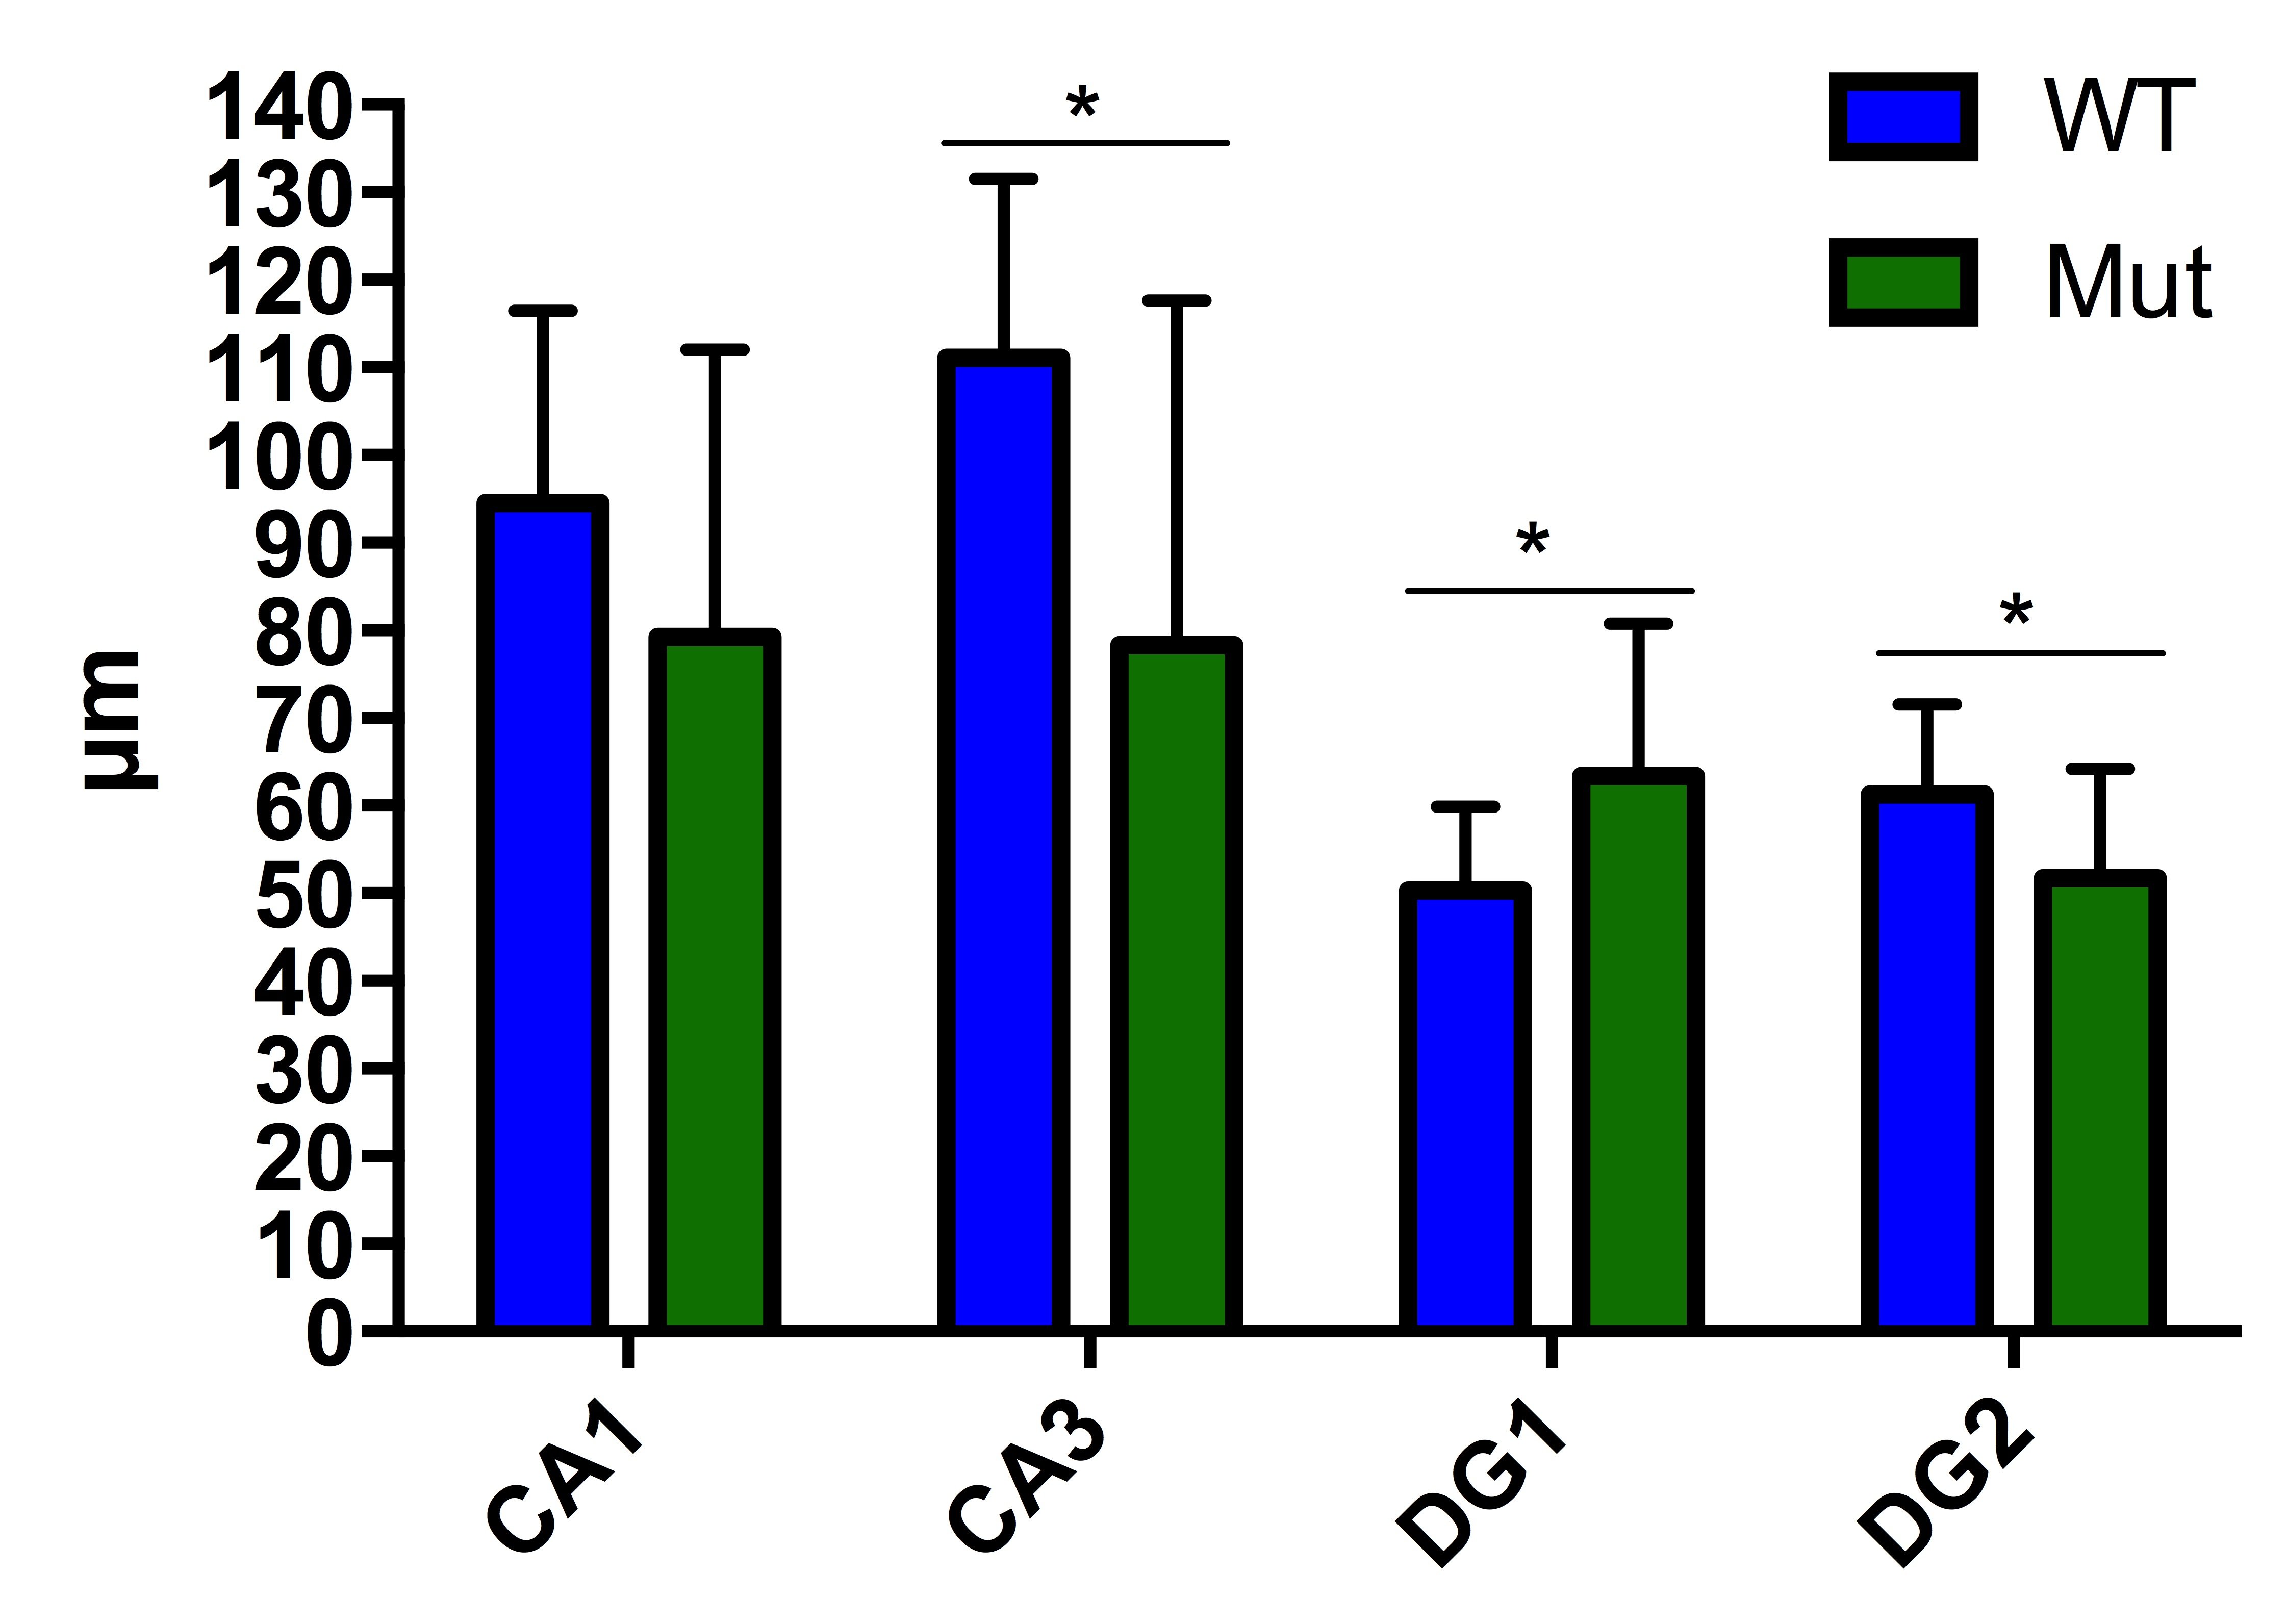
\includegraphics[width=\textwidth]{./Images/Immuno/NeuN/Qantif_Post.jpg}
			\end{subfigure}
			\caption{La distribution des neurones dans l'hippocampe est modifié par la mutation \mcrd.}
			\descfig{%
					Marquage de \acrshort{neun} sur tranche de cerveau. Illustration des différentes profondeurs choisies pour les mesures.
					\subref{fig:NeuNIllu1} Exemple de coupe rostrale.
					\subref{fig:NeuNIllu2} Exemple de coupe médiane.
					\subref{fig:NeuNIllu3} Exemple de coupe caudale.
					\subref{fig:hippIllu} Schéma des régions CA1, CA3, et DG 1 (zone suprapyramidale) \& 2 (zone infrapyramidale) dans lesquelles sont effectuées les mesures. Issue de Li et Pleasure, 2013 \cite{Li2013a}.
					\subref{fig:NeunQuantifNasal} Quantification de l'épaisseur de la couche pyramidale de différentes régions de l'hippocampe sur des coupes rostrales. 
					\subref{fig:NeunQuantifMilieu} Quantification sur des coupes médianes.
					\subref{fig:NeunQuantifPost} Quantification sur des coupes caudales.
					Ca : Cornus Ammonis, DG : Gyrus Denté. 
					Barre d'échelle : 2mm. 
					Test statistique : Test t de Student non apparié. 
					* : p<0.05, ** : p<0.01, *** : p<0.001. 
					n = 2 (\acrshort{wt}) et n = 3 (mutants).
					}
			\label{fig:NeuNResultat}
		\end{figure}
	\FloatBarrier
	
\section{Localisation et identification des cellules neurales exprimant \acrshort{musk}}
	\label{ssec:musk}
	Après avoir observé l'organisation globale du cerveau de souris et la distribution des neurones dans l'hippocampe, j'ai cherché à identifier les régions du cerveau exprimant \gls{musk}. Pour cela, j'ai eu recours à une technique d'immunohistochimie. L'anticorps utilisé est un anticorps polyclonal de lapin, dirigé contre le domaine extracellulaire de \gls{musk} (information donnée par le fournisseur).
	
	Malgré le fait que le niveau d'expression de \gls{musk} soit considéré comme faible dans le tissu nerveux d'après des études antérieurs (par northen blot principalement), j'ai quand même pu observer un marquage de cette protéine dans diverses régions discrètes du cerveau : Hippocampe (couche radiaire et moléculaire principalement) (\cref{fig:locaMuSKca1}), Corps calleux (\cref{fig:locaMuSKcc}), Habenula médiale (\cref{fig:locaMuSKhb}), Fasciculus retroflexus (\cref{fig:locaMuSKfr}), Capsule interne, Noyau caudé, 3ème ventricule ventrale, Cervelet principalement (\cref{fig:ImmunoMusk}). 
	
	\begin{figure}[h] %Figure Immuno MuSK Résultats
		\begin{subfigure}[h]{0.99\textwidth}
			\caption{}
			\label{fig:locaMusK}
			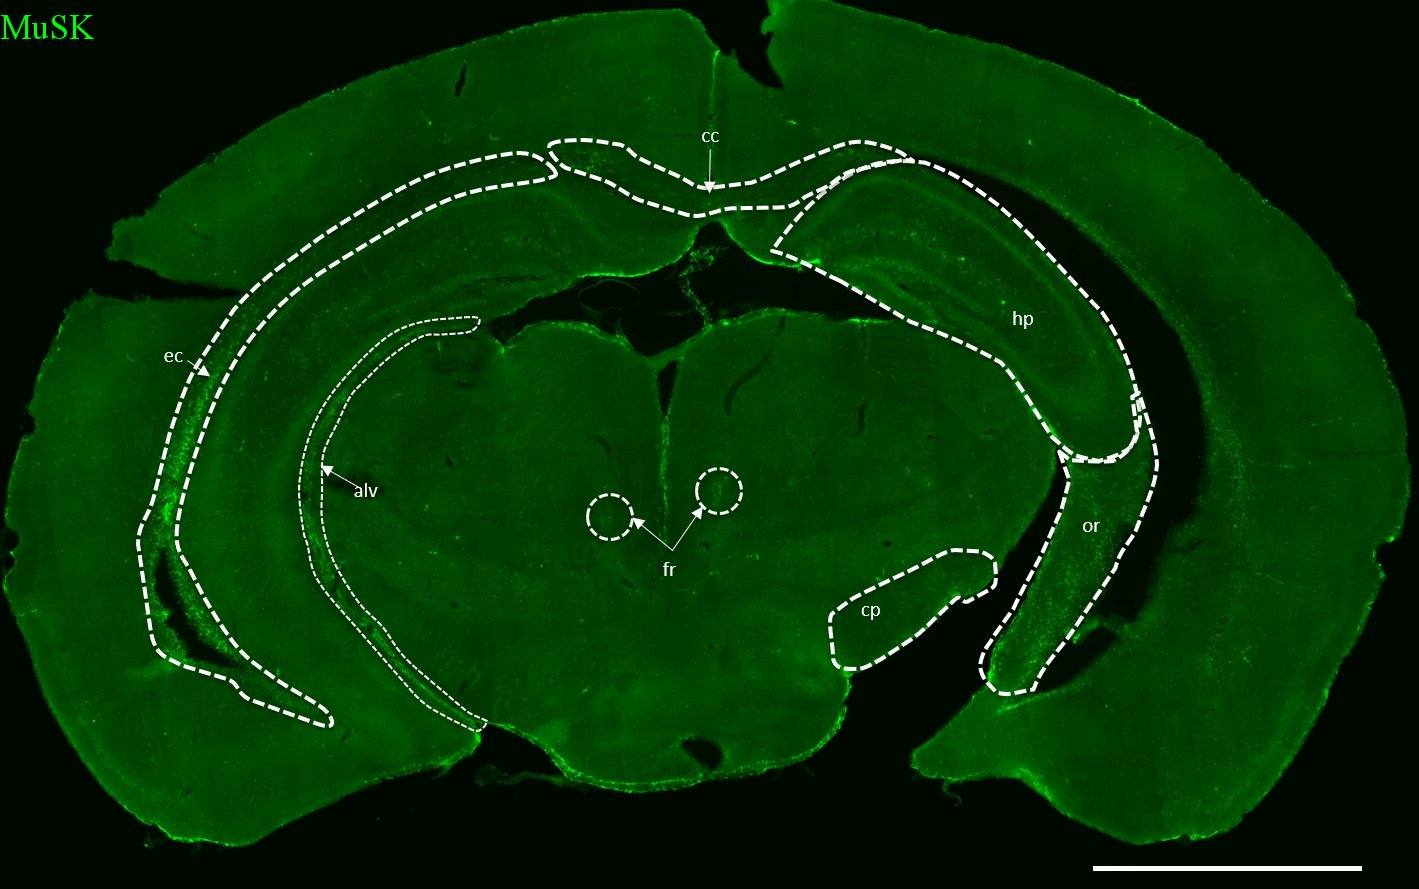
\includegraphics[width=\textwidth]{./Images/Immuno/Musk/loca_MuSK.jpg}
		\end{subfigure}
		\begin{subfigure}[h]{0.245\textwidth}
			\caption{}
			\label{fig:locaMuSKcc}
			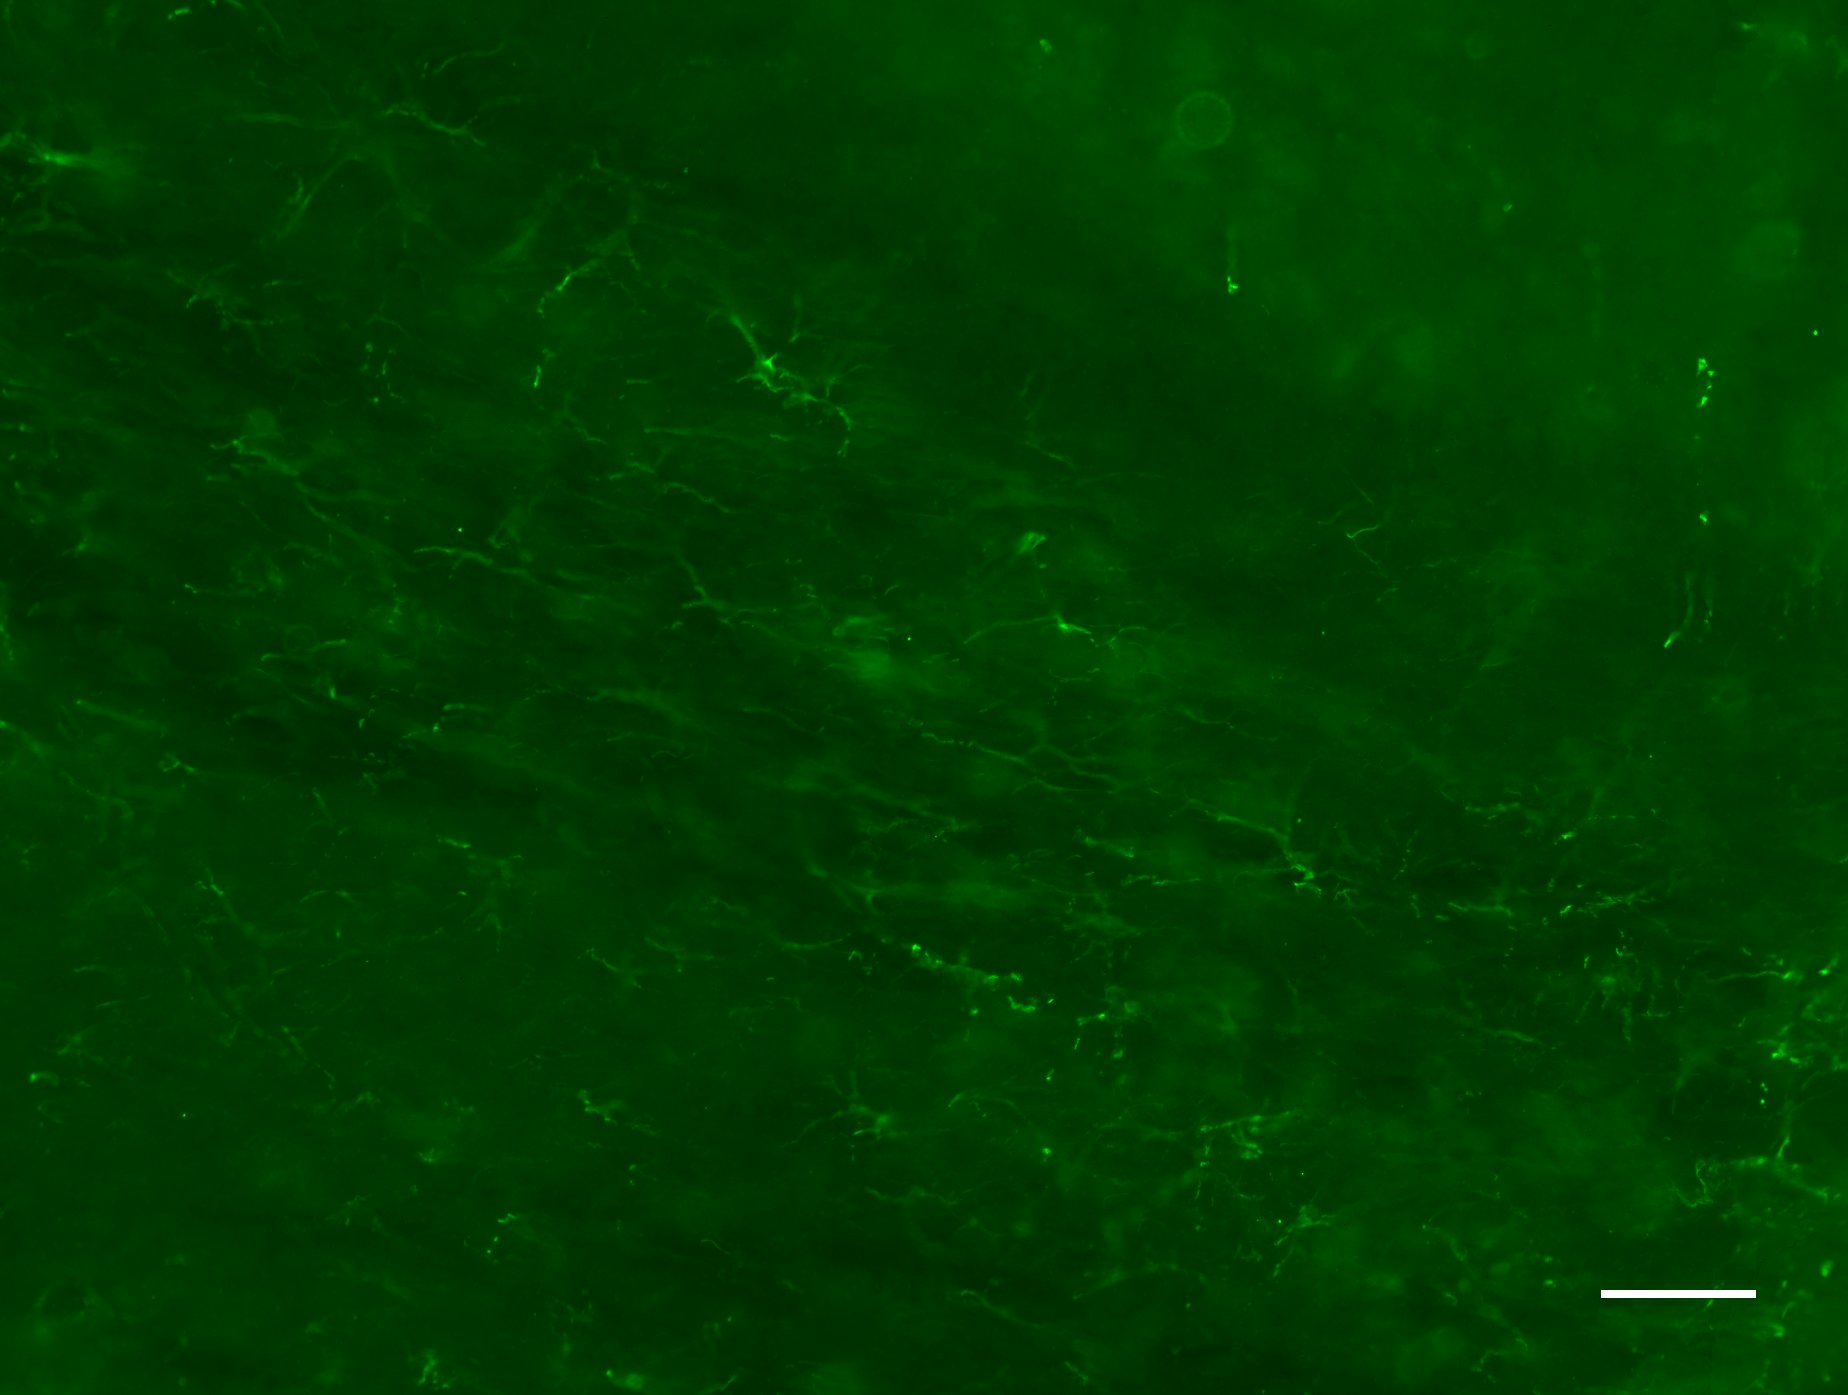
\includegraphics[width=\textwidth]{./Images/Immuno/Musk/MuSK_cc_50um.jpg}
		\end{subfigure}
		\begin{subfigure}[h]{0.245\textwidth}
			\caption{}
			\label{fig:locaMuSKca1}
			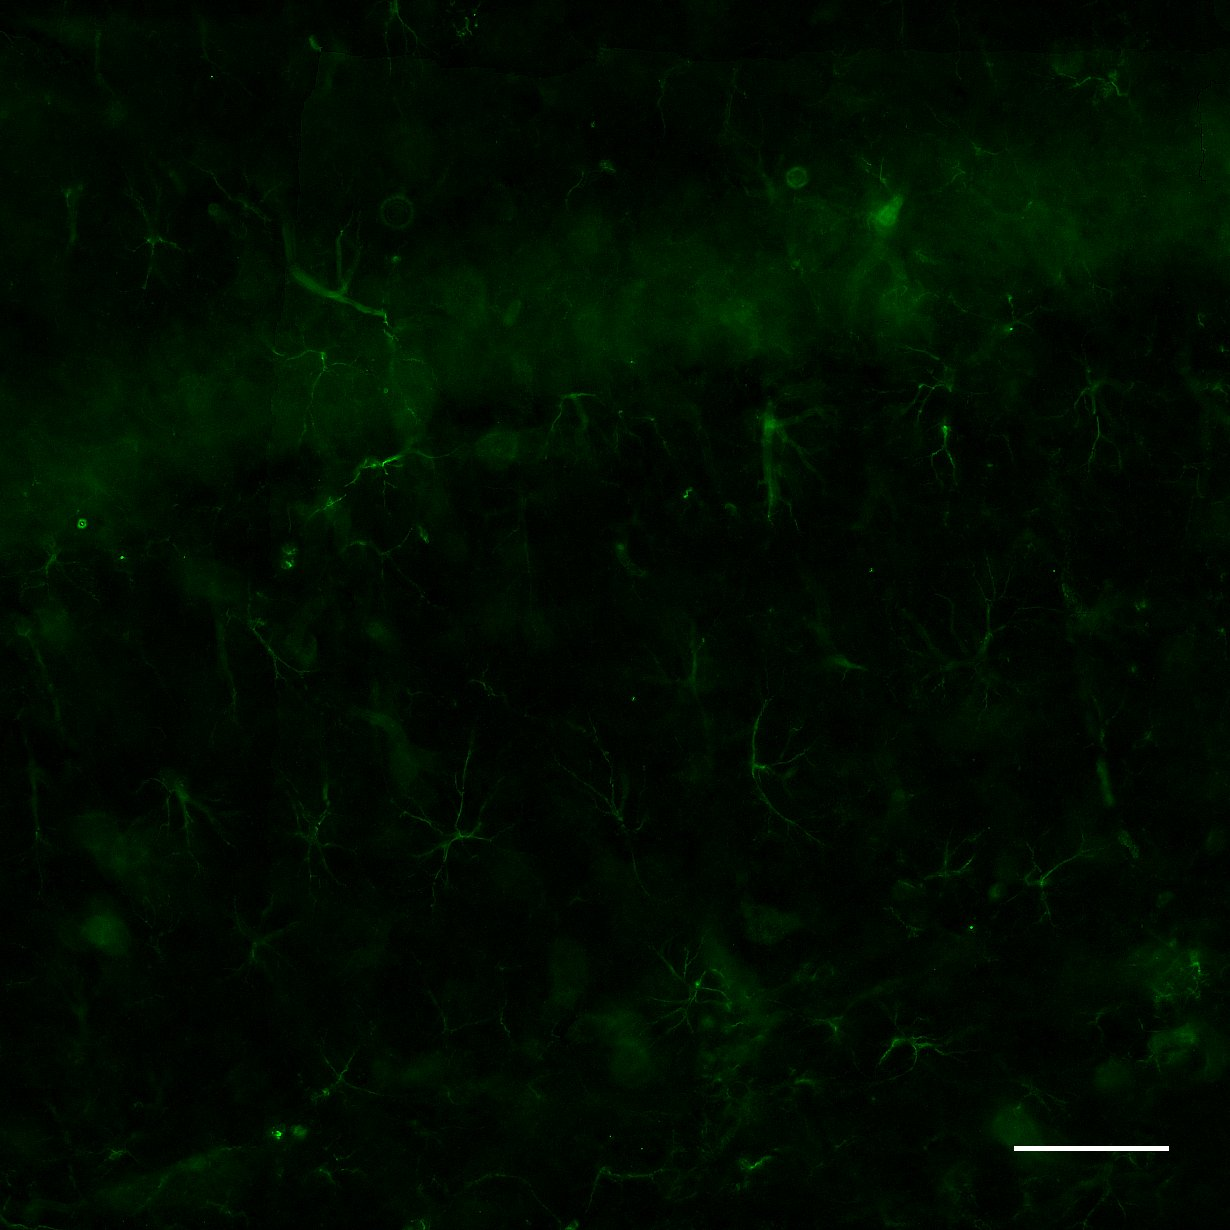
\includegraphics[width=\textwidth]{./Images/Immuno/Musk/MuSK_ca1_50um.jpg}
		\end{subfigure}
		\begin{subfigure}[h]{0.245\textwidth}
			\caption{}
			\label{fig:locaMuSKdg}
			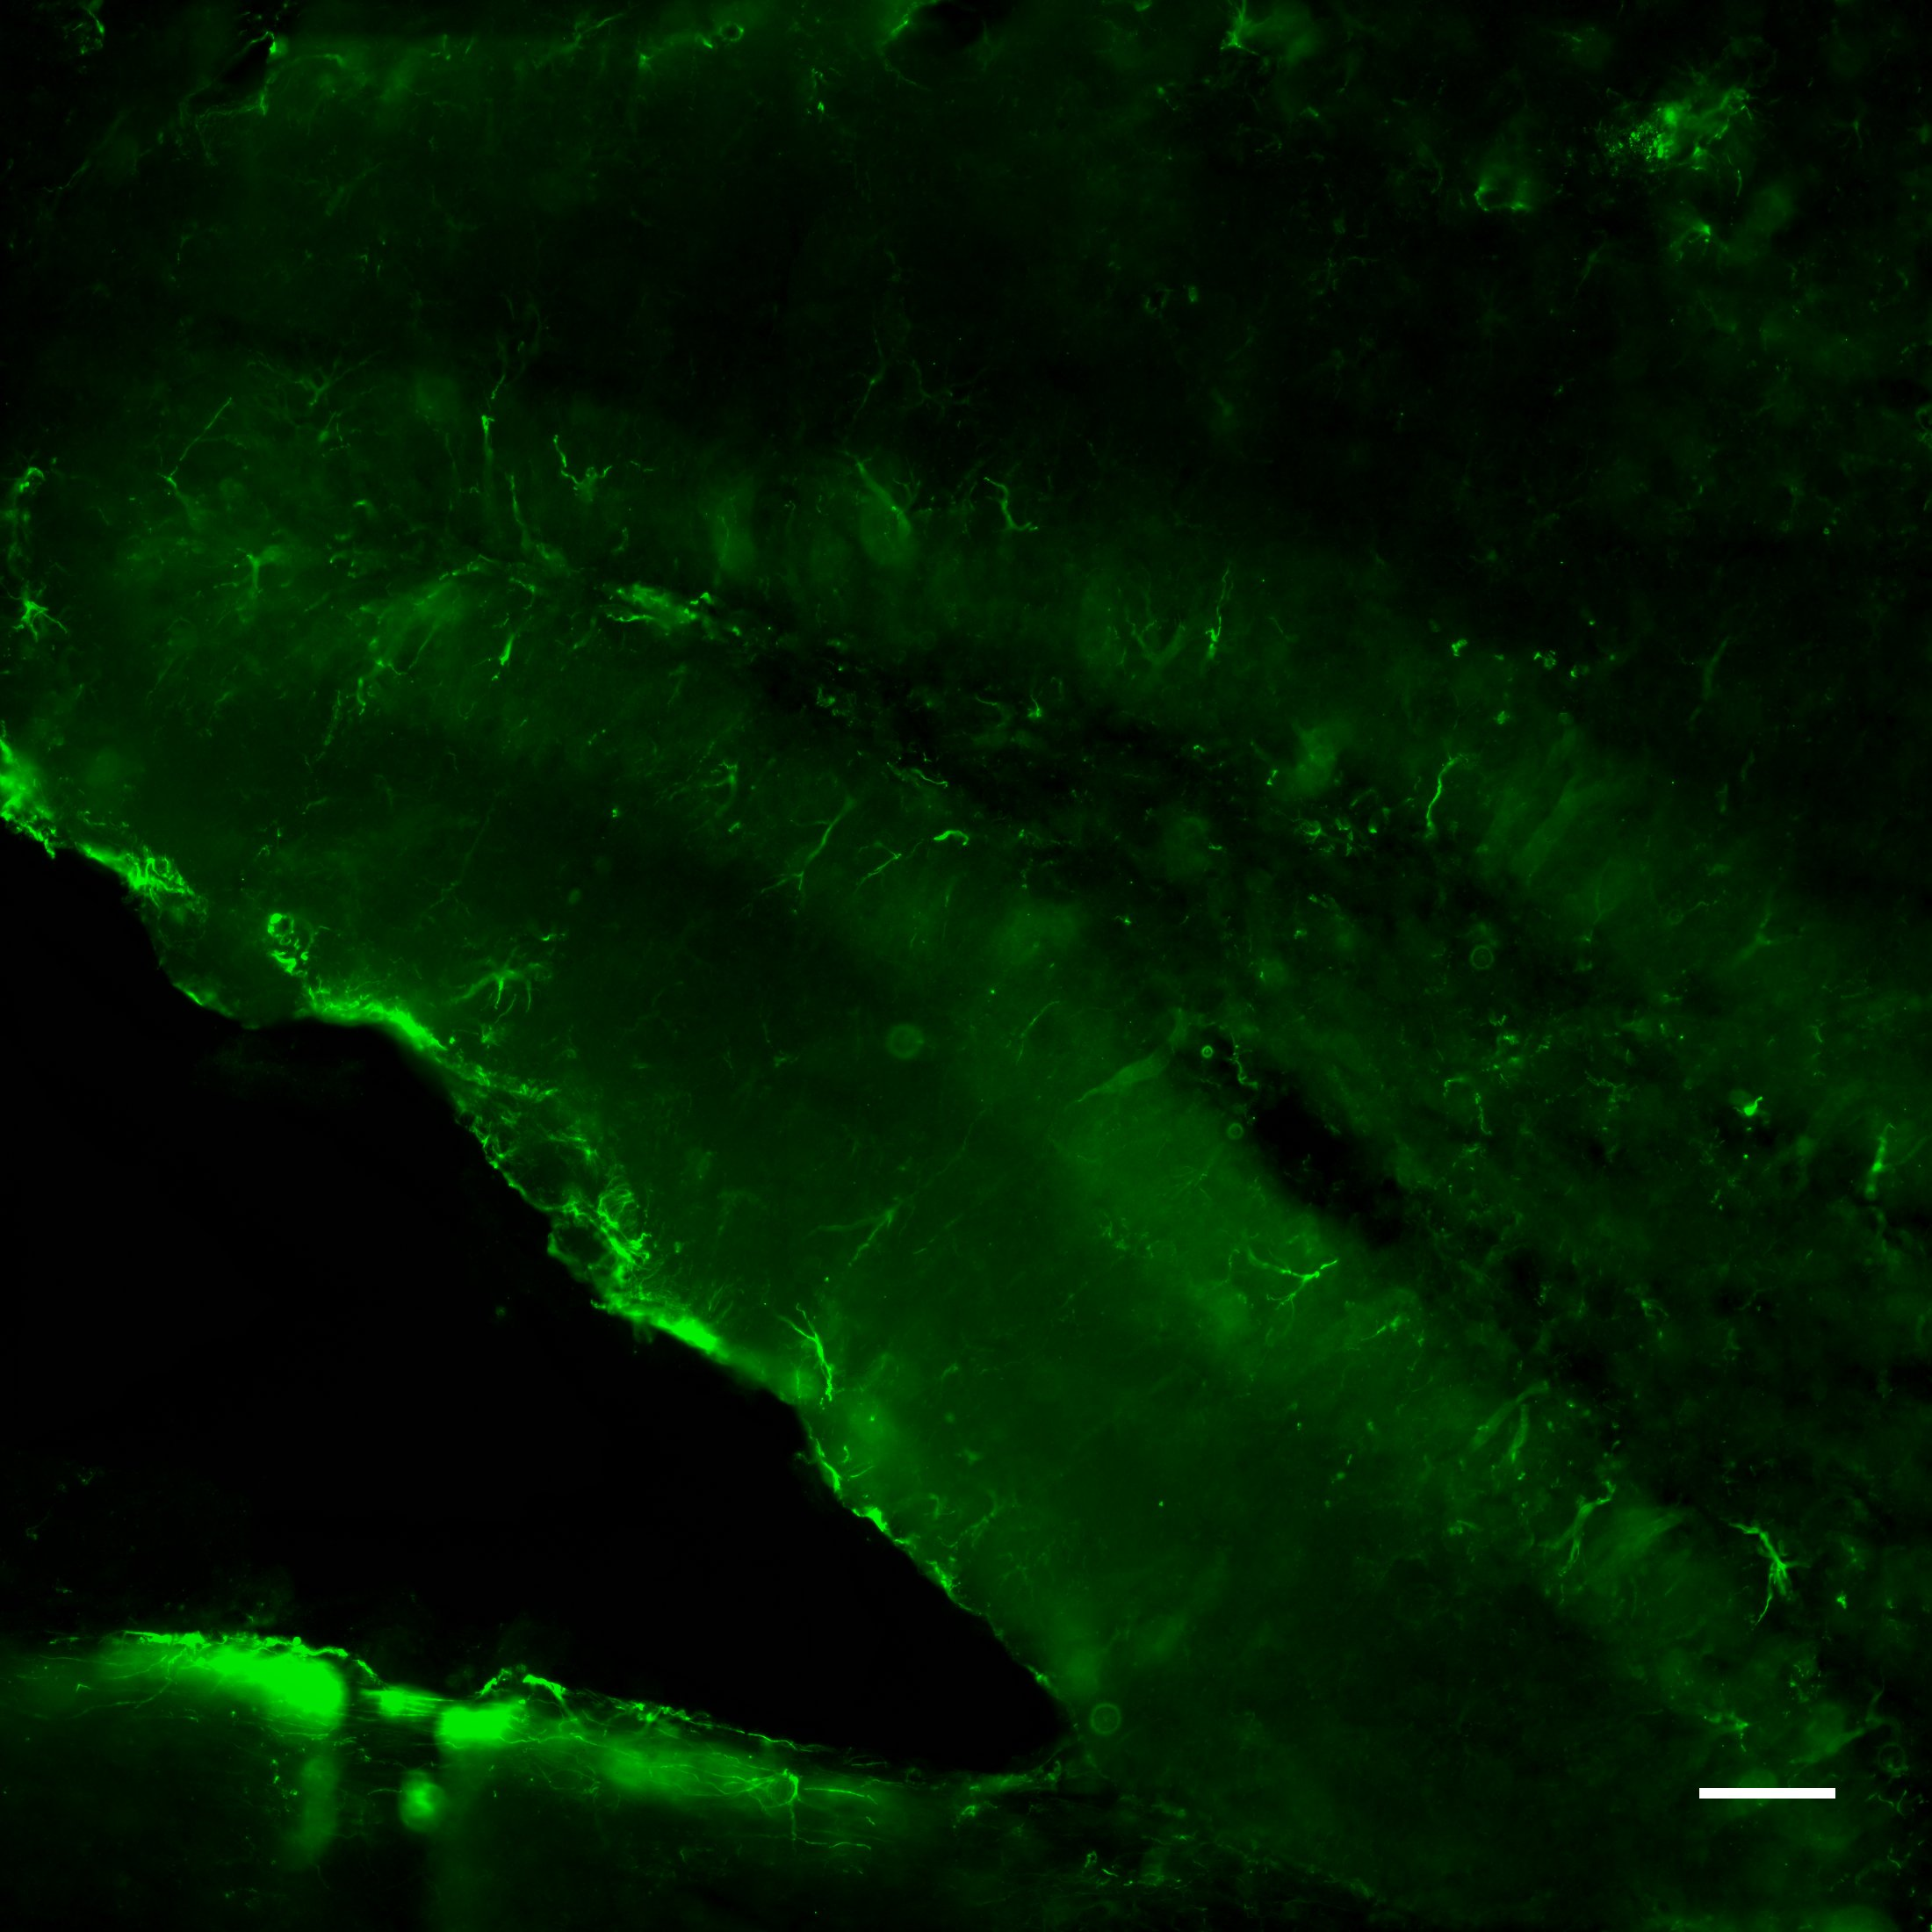
\includegraphics[width=\textwidth]{./Images/Immuno/Musk/MuSK_dg_50um.jpg}
		\end{subfigure}
		\begin{subfigure}[h]{0.245\textwidth}
			\caption{}
			\label{fig:locaMuSKhb}
			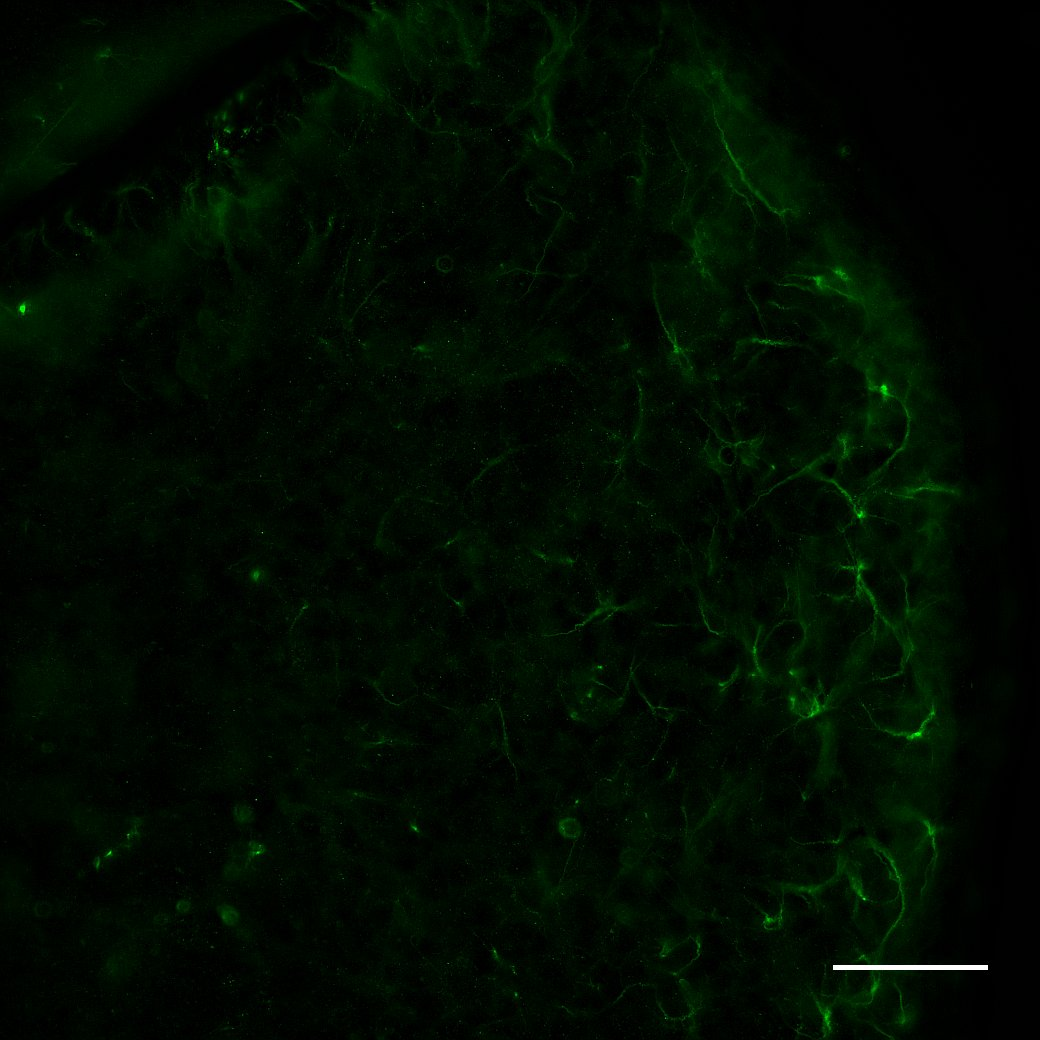
\includegraphics[width=\textwidth]{./Images/Immuno/Musk/MuSK_hb_50um.jpg}
		\end{subfigure}
		\begin{subfigure}[h]{0.245\textwidth}
			\caption{}
			\label{fig:locaMuSKfr}
			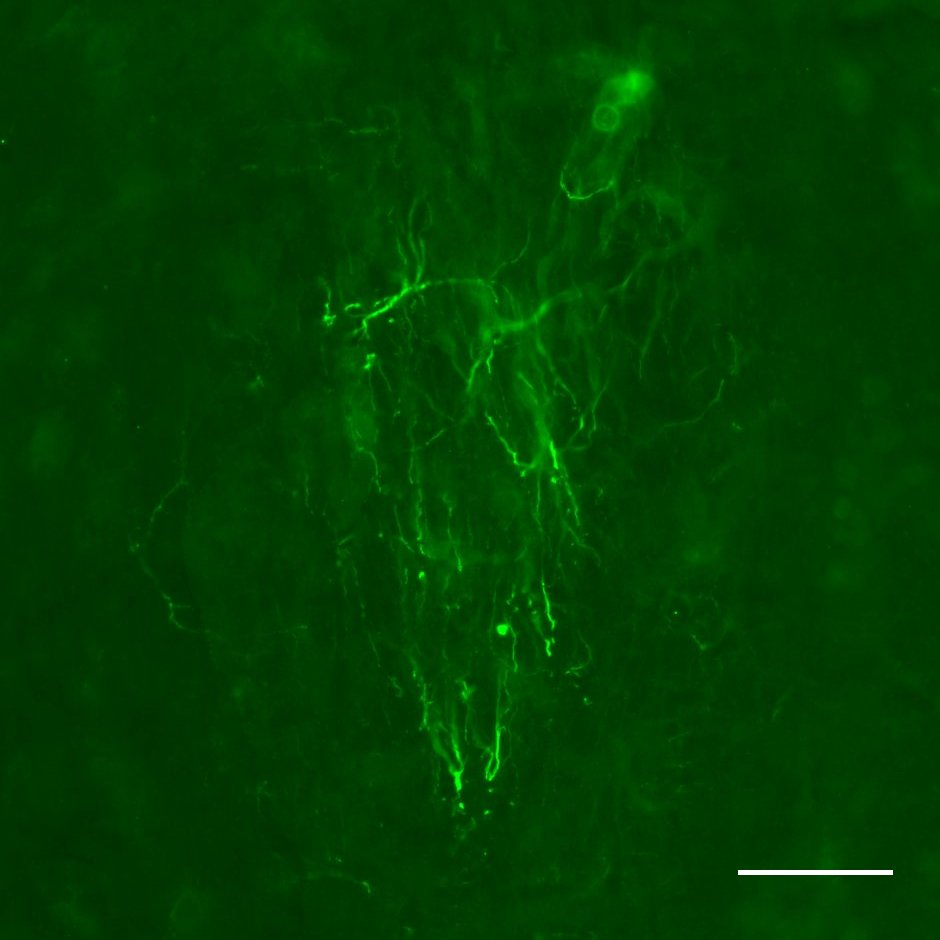
\includegraphics[width=\textwidth]{./Images/Immuno/Musk/MuSK_fr_50um.jpg}
		\end{subfigure}
		\begin{subfigure}[h]{0.395\textwidth}
			\caption{}
			\label{fig:locaMusKCtrl}
			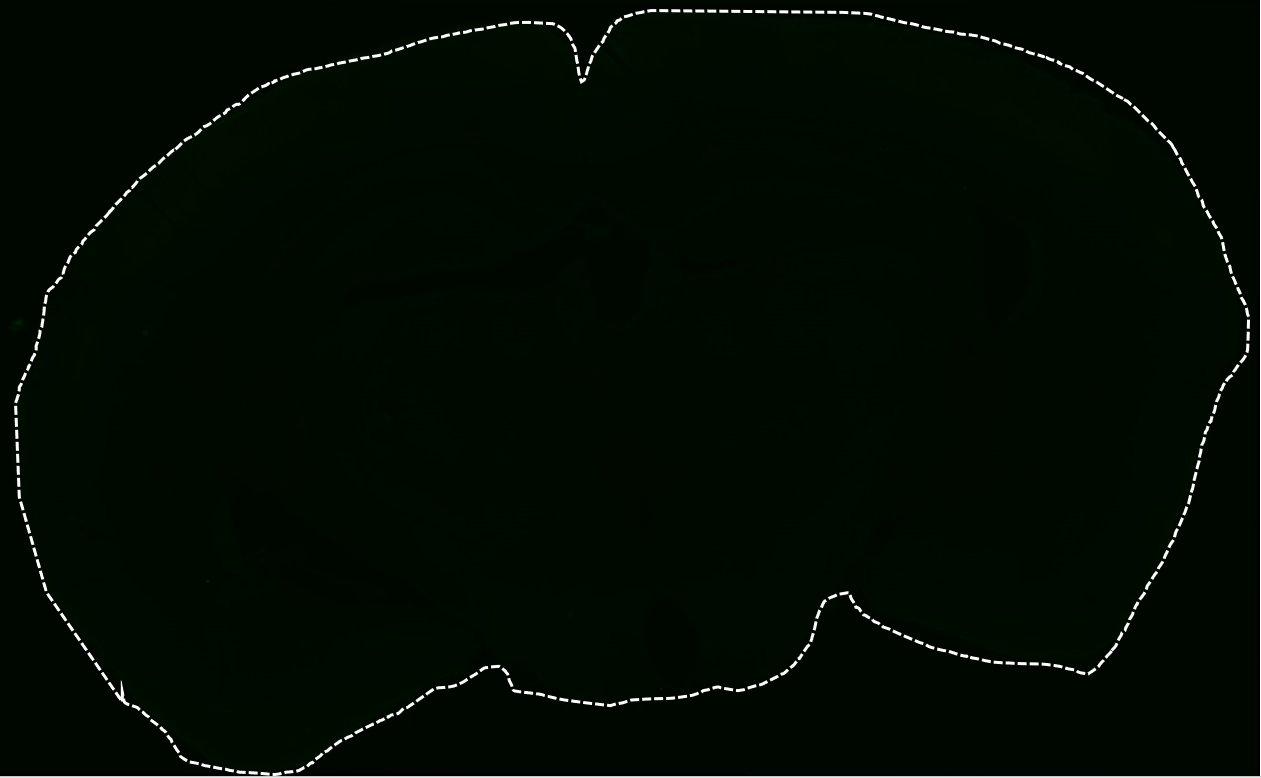
\includegraphics[width=\textwidth]{./Images/Immuno/Musk/loca_MuSK_ctrl.jpg}
		\end{subfigure}
		\caption{Localisation de \gls{musk} dans le cerveau.}
		\descfig{%
			\subref{fig:locaMusK} Immunomarquage de \gls{musk} sur coupe de cerveau entière. Coupe de souris mutante, mais le marquage est semblable chez les souris sauvages. %
			\subref{fig:locaMuSKcc} Grossissement sur l'organisation du marquage au niveau du corps calleux. %
			\subref{fig:locaMuSKca1} Grossissement sur l'organisation du marquage au niveau de la région CA1. L'épaississement vert correspond à la présence de noyau de la couche pyramidale. %
			\subref{fig:locaMuSKdg} Grossissement sur l'organisation du marquage au niveau du Gyrus Denté. %
			\subref{fig:locaMuSKhb} Grossissement sur l'organisation du marquage au niveau de l'habenula médiale. %
			\subref{fig:locaMuSKfr} Grossissement sur l'organisation du marquage au niveau du fasciculus retroflexus. %
			\subref{fig:locaMusKCtrl} Coupe contrôle du marquage de \gls{musk} dans un cerveau de souris \mcrd. Aucun marquage n'apparaît. %
			 alv : alveus hippocampus, cc : corps calleux, cp : pédoncule cérébral, ec : capsule externe, fr : fasciculus retroflexus, hp : hippocampe, or : stratum oriens de l'hippocampe. Barre d'échelle : 2 mm (\subref{fig:locaMusK}, \subref{fig:locaMusKCtrl}), 50µm (\subref{fig:locaMuSKcc}- \subref{fig:locaMuSKfr}).
			 	}
		\label{fig:ImmunoMusk}
	\end{figure}
	
	Dans ces régions, \gls{musk} est présent dans des prolongements cellulaires. La structure des cellules marquées par l'anticorps anti-\gls{musk} étant réminiscente de celles des astrocytes, un co-marquage de \gls{musk} et \gls{gfap}, une protéine spécifique du cytosquelette des astrocytes a été réalisé.
	
	Pour réaliser le marquage de \gls{gfap}, deux anticorps différents ont été utilisés. Le premier, fourni par l'équipe de C. Agulhon, provient de chez Millipore-Merck (\cref{table:Ac}, réf. MAB360) et a permis de visualiser des marquages spécifique. Le second anticorps, provenant de chez Abcam (\cref{table:Ac}, réf. ab4648) et commandé suite à une indisponibilité du premier anticorps, n'a révélé aucune marquage à différentes concentrations testées ($1{:}100$, $1{:}50$). Le premier anticorps a été utilisé dans l'ensemble des expériences.
	
	Suite au co-marquage de \gls{musk} et \gls{gfap}, on peut observer une colocalisation des deux marqueurs, ce qui semblerait indiqué que \gls{musk} est exprimé par les astrocytes (\cref{fig:ColocMuSK,fig:ColocGFAP,fig:ColocMuSK&GFAP}). 
	
	F. Semprez, un autre membre de l'équipe, a montré qu'en plus du cerveau, \gls{musk} est également présent dans la substance blanche de la moëlle épinière, et colocalise avec \gls{gfap} (\cref{fig:MuSKME}).
	
	%Images Coloc. MuSK GFAP
	\begin{figure}[h]
		\begin{subfigure}[h]{0.329\textwidth}
			\caption{}
			\label{fig:ColocMuSK}
			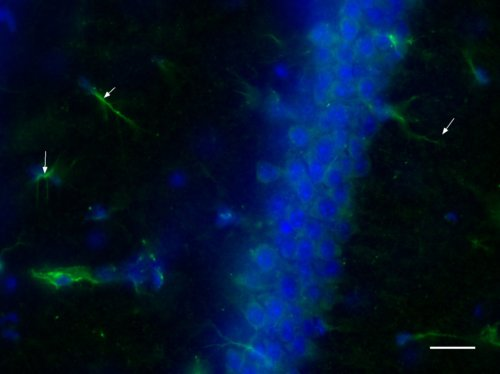
\includegraphics[width=\textwidth]{./Images/Immuno/Musk/MuSK-GFAP/M439_Mut_MuSK.jpg}
		\end{subfigure}
		\begin{subfigure}[h]{0.329\textwidth}
			\caption{}
			\label{fig:ColocGFAP}
			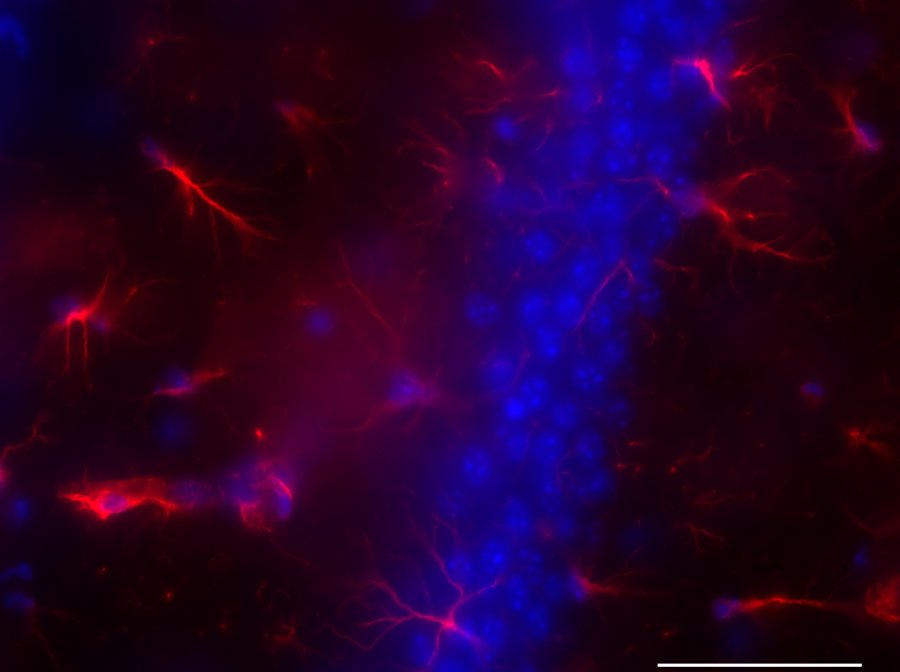
\includegraphics[width=\textwidth]{./Images/Immuno/Musk/MuSK-GFAP/M439_Mut_GFAP.jpg}
		\end{subfigure}
		\begin{subfigure}[h]{0.329\textwidth}
			\caption{}
			\label{fig:ColocMuSK&GFAP}
			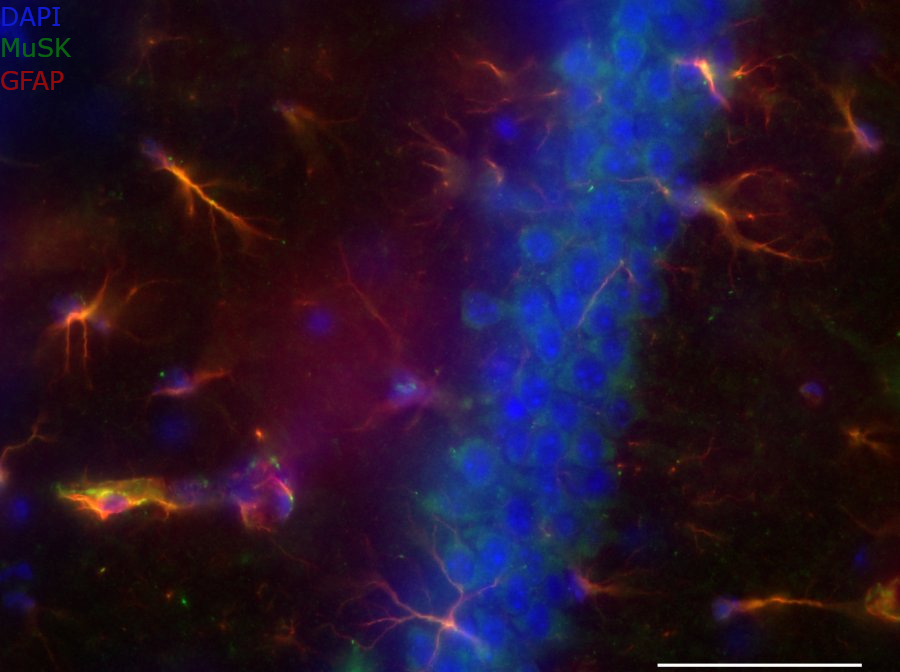
\includegraphics[width=\textwidth]{./Images/Immuno/Musk/MuSK-GFAP/M439_Mut_MuSK_GFAP.jpg}
		\end{subfigure}
		\begin{subfigure}[h]{0.329\textwidth}
			\caption{}
			\label{fig:ColocZoom}
			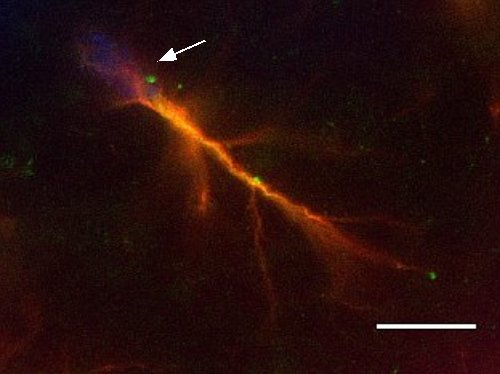
\includegraphics[width=\textwidth]{./Images/Immuno/Musk/MuSK-GFAP/zoom10um.jpg}
		\end{subfigure}
		\begin{subfigure}[h]{0.329\textwidth}
			\caption{}
			\label{fig:MuSKME}
			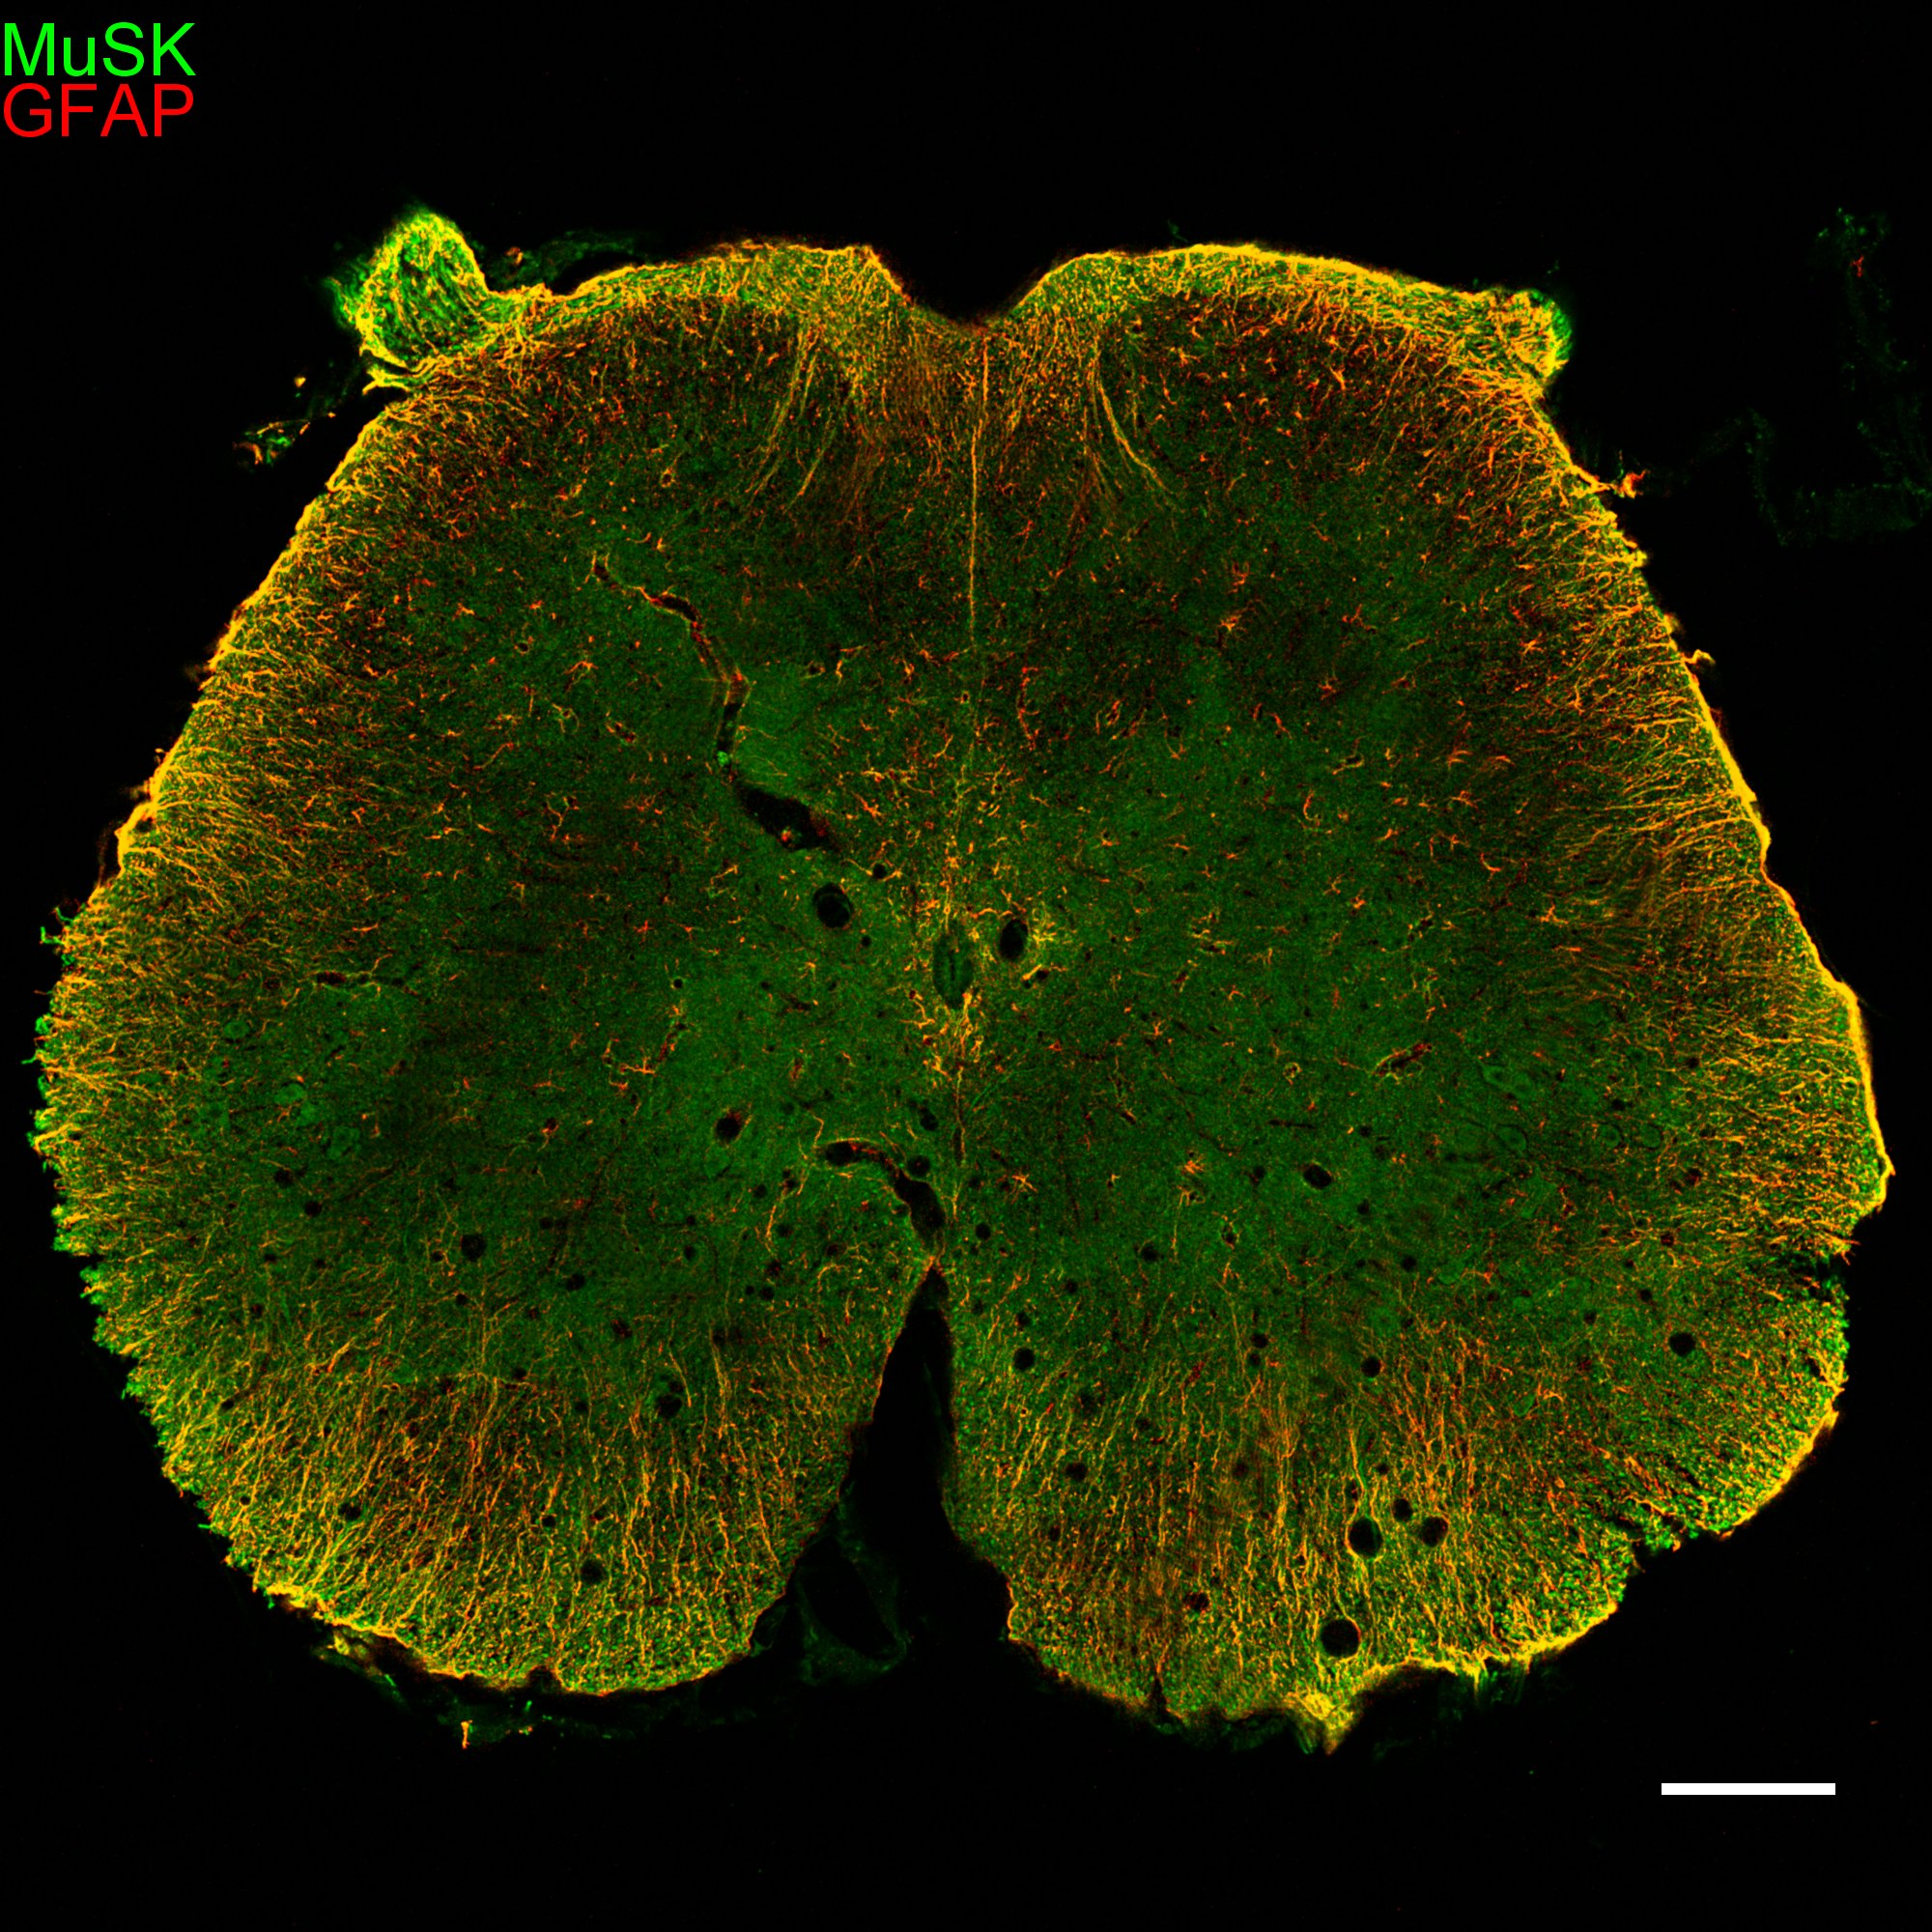
\includegraphics[width=\textwidth]{./Images/Immuno/Musk/Moelle_MuSK_GFAP_150um.jpg}
		\end{subfigure}
		\caption{\gls{musk} et \gls{gfap} colocalisebt dabs les mêmes cellules.}
		\descfig{%
			Marquage de \gls{musk} (vert) et de \gls{gfap} (rouge) et \acrshort{dapi} (bleu) au niveau de la région CA1 de l'hippocampe. Le marquage de \gls{musk} colocalise avec \gls{gfap} dans toutes les régions du cerveau observées.
			\subref{fig:ColocMuSK} Marquage de \gls{musk}.
			\subref{fig:ColocGFAP} Marquage de \gls{gfap}.
			\subref{fig:ColocMuSK&GFAP} Superposition de \subref{fig:ColocMuSK} et \subref{fig:ColocGFAP}.
			\subref{fig:ColocZoom} Zoom de la partie encadré de \subref{fig:ColocMuSK&GFAP}. On peut observer que le prolongement marqué à la fois par \gls{musk} et \gls{gfap} semblent se mettrent en place autour d'un noyau (flèche blanche).
			\subref{fig:MuSKME} Co-marquage de \gls{musk} et de \gls{gfap} au niveau de la moëlle épinière.
			Barre d'échelle : 150µm \subref{fig:MuSKME} ; 20µm \subref{fig:ColocMuSK}, \subref{fig:ColocGFAP}, \subref{fig:ColocMuSK&GFAP} ; 10µm \subref{fig:ColocZoom}.
				}	
		\label{fig:colocalisation}
	\end{figure}
%\FloatBarrier
	
	Cependant, le marquage observé de \gls{musk} ne ressemble pas à ce que l'on peut observer au niveau de la \gls{jnm}, où \gls{musk} est observé uniquement au niveau du domaine post-synaptique. L'observation d'un marquage continue dans des prolongements astrocytaires nous à amené à nous poser la question de la spécificité de l'anticorps anti-\gls{musk}. Comme il n'existe pas d'autres anticorps dirigés contre \gls{musk} utilisables en \gls{ihc}, j'ai dû essayer d'autres approches afin de tenter de confirmer la spécificité du marquage. Tout d'abord, un co-marquage \gls{musk}/\acrshort{gfap} à été réalisé sur des sections de cerveau d'embryon de souris \gls{musk} KO (stade E18.5), la mutation étant létale après la naissance pour cause de défaillance respiratoire (\cref{fig:MuskEmbryon}). Sur seulement une coupe d'embryon \gls{wt}, un léger marquage ressemblant à celui observé chez les adultes est présent (\cref{fig:MuskE5WT,fig:MuskE5Marquage}), et aucun marquage n'est présent chez les animaux KO (\cref{fig:MuskE1KO}). Cela ne suffit pas à confirmer la spécificité du marquage de \gls{musk}, les astrocytes n'aparaissant qu'après la naissance. Pour tenter alors de confirmer la présence de \gls{musk} dans le cerveau, une immunoprécipitation a été alors envisagée (voire partie \cref{sec:IPresultat}).
	
	%Images Embryon
	\begin{figure}[h]
		\begin{center}
			\begin{subfigure}[h]{0.329\textwidth}
				\caption{}
				\label{fig:MuskE5WT}
				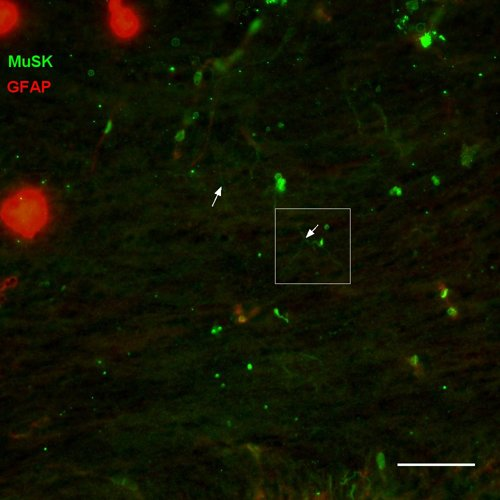
\includegraphics[width=\textwidth]{./Images/Immuno/Musk/Embryon/E5WT_50um_500px_df.jpg} 
			\end{subfigure}
			\begin{subfigure}[h]{0.329\textwidth}
				\caption{}
				\label{fig:MuskE5Marquage}
				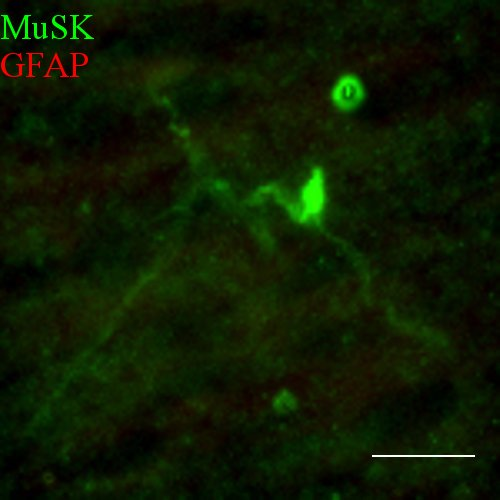
\includegraphics[width=\textwidth]{./Images/Immuno/Musk/Embryon/E5_WT_MuSK_500px_Zoom_10um.jpg}
			\end{subfigure}
			\begin{subfigure}[h]{0.329\textwidth}
				\caption{}
				\label{fig:MuskE1KO}
				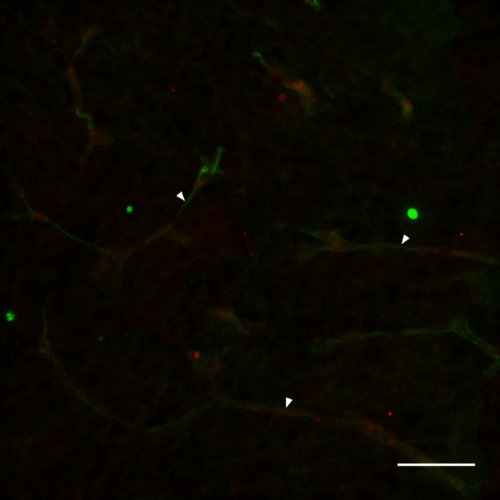
\includegraphics[width=\textwidth]{./Images/Immuno/Musk/Embryon/E1KO_50um_500px_df.jpg}
			\end{subfigure}
		\end{center}
		\caption{Pas de marquage de \gls{musk} sur embryon E18.5 WT et KO.}
		\descfig{%
			Marquage de \gls{musk} et \gls{gfap} sur des embryons (stade E18.5) de souris \gls{musk} KO (n = 2) et WT (n = 1). Aucun marquage de \gls{gfap} n'est visible car les astrocytes n'apparaissent qu'après la naissance. %
			\subref{fig:MuskE5WT} Embryon WT. Sur une coupe, un marquage ressemblant à celui de \gls{musk} observé chez les adultes était présent (flèches blanches). %
			\subref{fig:MuskE5Marquage} Agrandissement du marquage de \gls{musk}/\gls{gfap} encadré en \subref{fig:MuskE5WT}. %
			\subref{fig:MuskE1KO} Embryon KO. Le marquage observé (triangles blanc) n'est pas spécifique. %
			Images représentatives issues de la région du fornix dorsal. Barre d'échelle : 50µm \subref{fig:MuskE5WT} et  \subref{fig:MuskE1KO}, 10µm \subref{fig:MuskE5Marquage}. 
				}
		\label{fig:MuskEmbryon}
	\end{figure}
\FloatBarrier

	Afin d'identifier plus précisément le ou les types de cellules exprimant \gls{musk}, un co-marquage entre le récepteur et différents marqueurs a été réalisé sur des cultures primaires d'hippocampes, cultures issues d'embryon au stade E16 puis cultivées 14 jours, fournies par D. Carrel. Les marqueurs cellulaires sont \gls{gfap} pour marquer les astrocytes et \gls{map2} pour visualiser les dendrites des neurones. J'ai également testé un co-marquage \gls{musk} et \gls{glt1}, marqueur membranaire astrocytaire d'un transporteur du glutamate, afin de voir si \gls{musk} était localisé à la membrane, mais ce marquage n'a pas fonctionné.
	
	Les co-marquages de cultures cellulaires ont permis de confirmer la localisation observée sur les coupes de cerveaux de \gls{musk} : le récepteur est présent dans les prolongements astrocytaires (\cref{fig:CultureMGgfapmusk}). On peut voir sur les cultures les corps cellulaires des astrocytes, qui sont marqués à la fois par \gls{musk} et par \gls{gfap}, chose qui n'était pas visible lors de l'immunomarquage des coupes de cerveau.
	
	On observe également sur les images des prolongements cellulaires marqués par \gls{musk} qui ne sont pas co-marqués avec la \gls{gfap}. \gls{map2} est un marqueur des dendrites et du soma des neurones. Lors du co-marquage avec \gls{musk}, on peut voir sur les cultures certains prolongements sont à la fois marqués par \gls{map2} et par \gls{musk} (\cref{fig:CultureMMmap2}). On peut obserber un marquage de \gls{musk} dans des prolongements non marqués par \gls{map2}, qui sont vraisemblablement ceux des astrocytes au vu de leur morphologie. En plus du marquage de prolongements, \gls{map2} va aussi être présent  dans le soma, autour de noyaux (\cref{fig:CultureMMmap2musk}, flèches blanches) et va être co-localisé avec \gls{musk}. 
	
	%Images cultures cellulaire
	\clearpage	
	\begin{figure}
		\begin{subfigure}[h]{0.329\textwidth}
			\caption{}
			\label{fig:CultureMGmusk}
			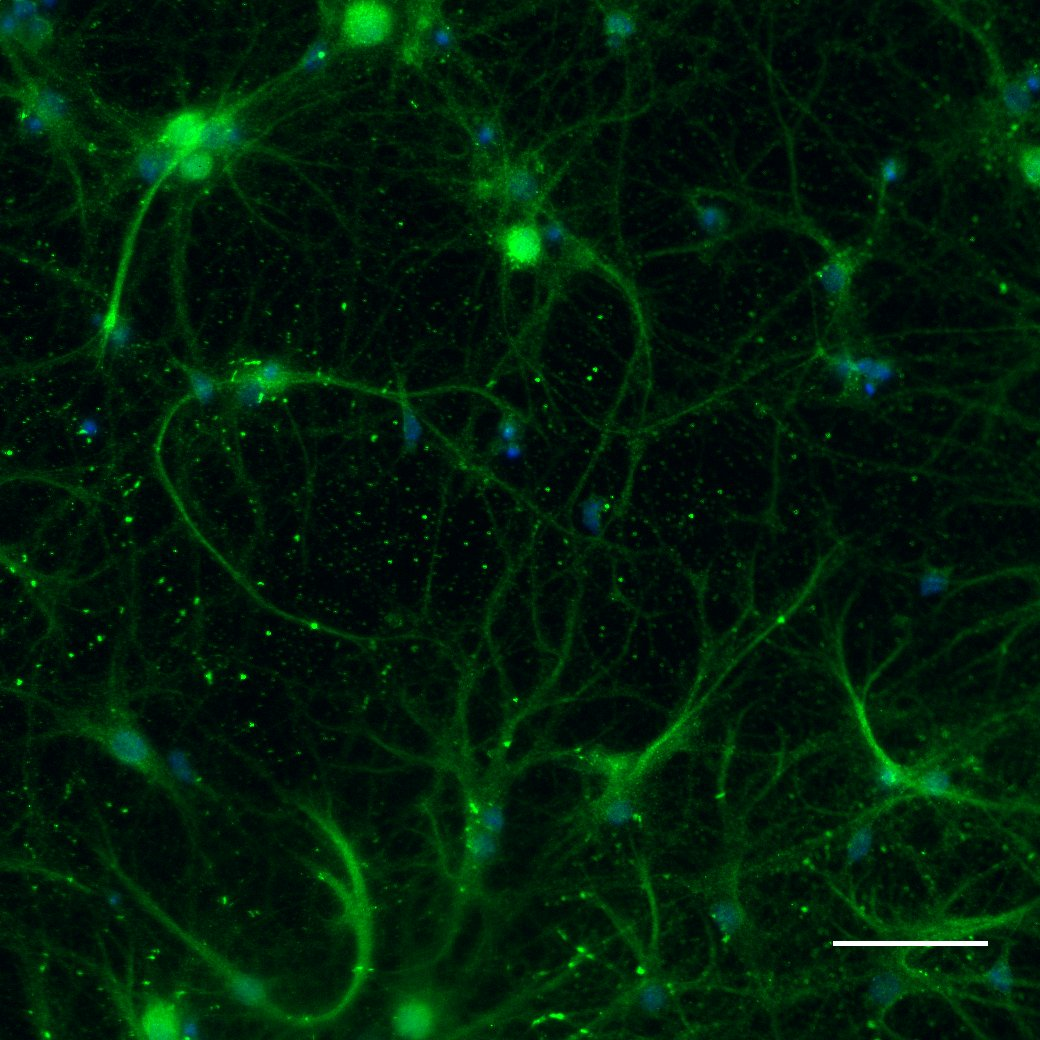
\includegraphics[width=\textwidth]{./Images/Immuno/Musk/Cultures/MuSK_50um.jpg}
		\end{subfigure}
		\begin{subfigure}[h]{0.329\textwidth}
			\caption{}
			\label{fig:CultureMGgfap}
			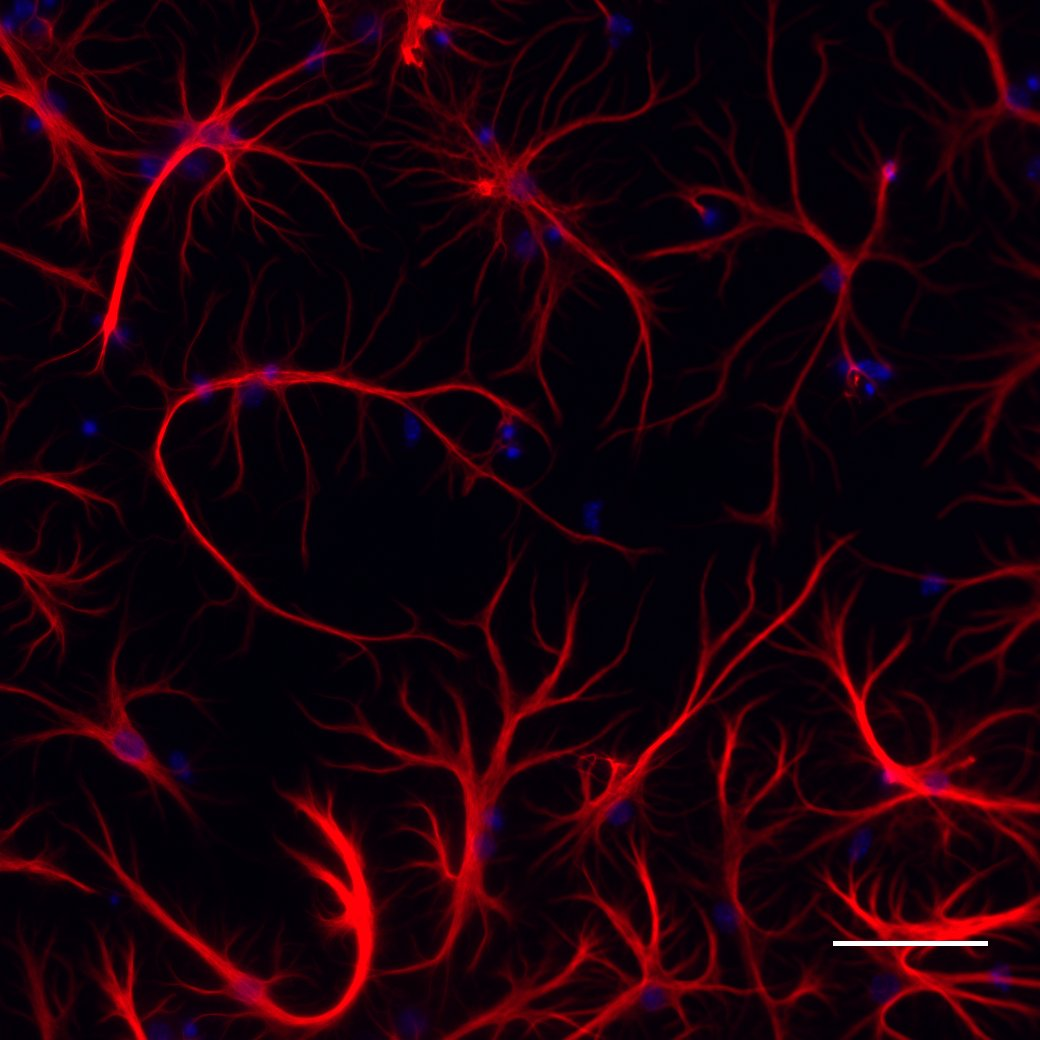
\includegraphics[width=\textwidth]{./Images/Immuno/Musk/Cultures/GFAP_50um.jpg}
		\end{subfigure}
		\begin{subfigure}[h]{0.329\textwidth}
			\caption{}
			\label{fig:CultureMGgfapmusk}
			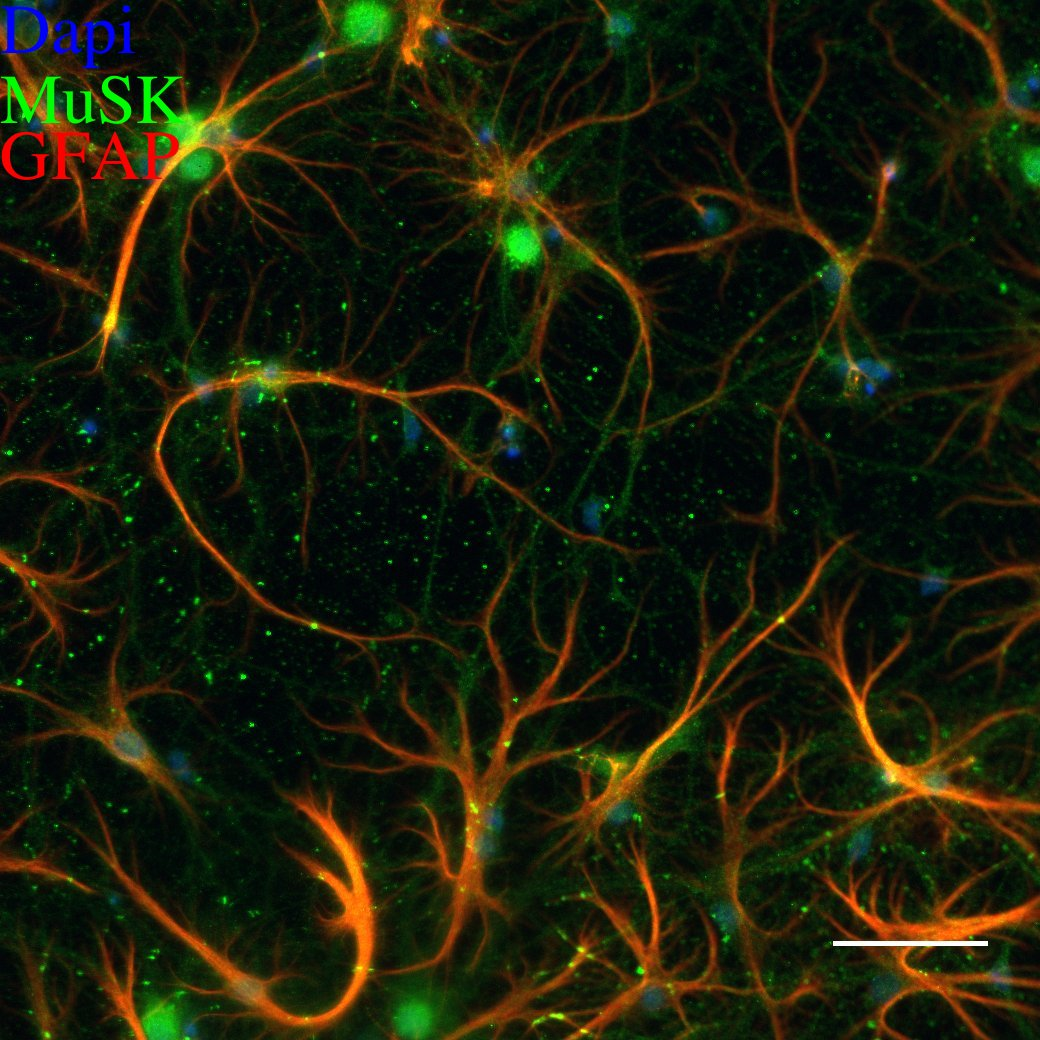
\includegraphics[width=\textwidth]{./Images/Immuno/Musk/Cultures/GFAP-MuSK_50um.jpg}
		\end{subfigure}
		\begin{subfigure}[h]{0.329\textwidth}
			\caption{}
			\label{fig:CultureMMmusk}
			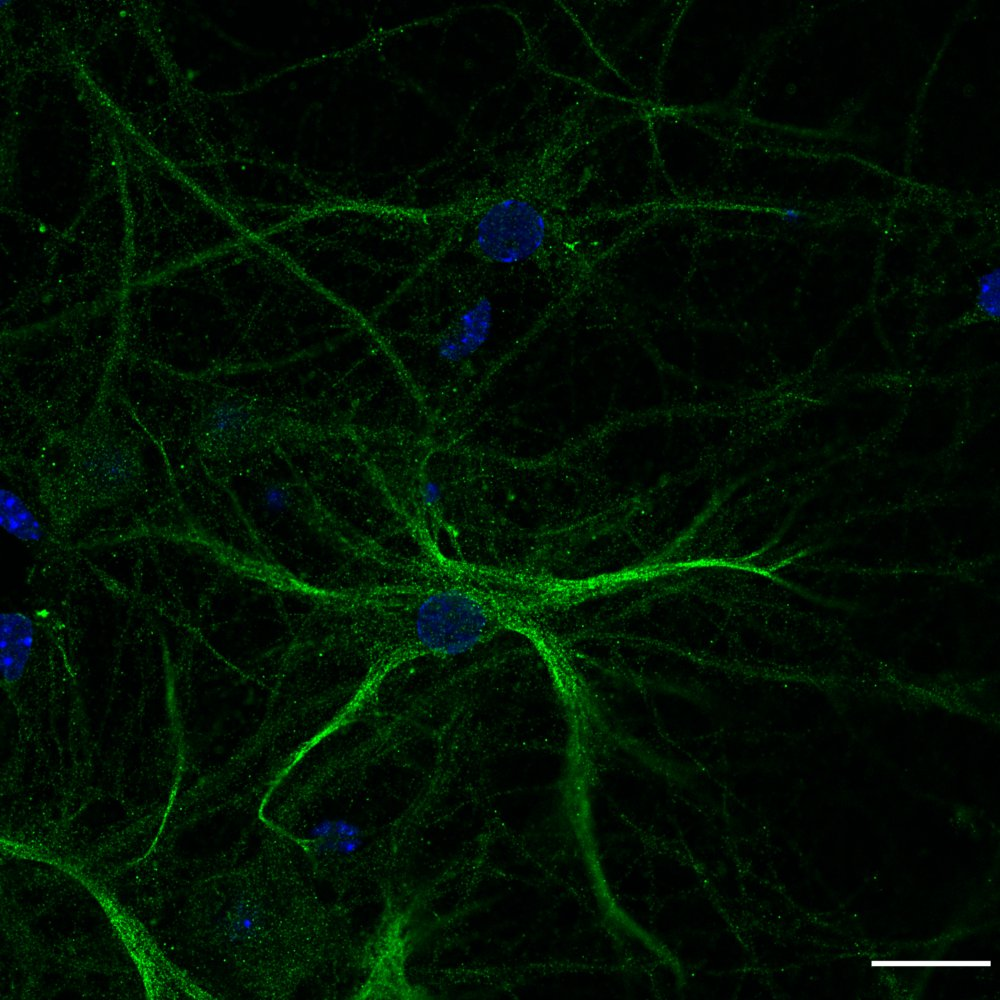
\includegraphics[width=\textwidth]{./Images/Immuno/Musk/Cultures/MuSK_20um.jpg}
		\end{subfigure}
		\begin{subfigure}[h]{0.329\textwidth}
			\caption{}
			\label{fig:CultureMMmap2}
			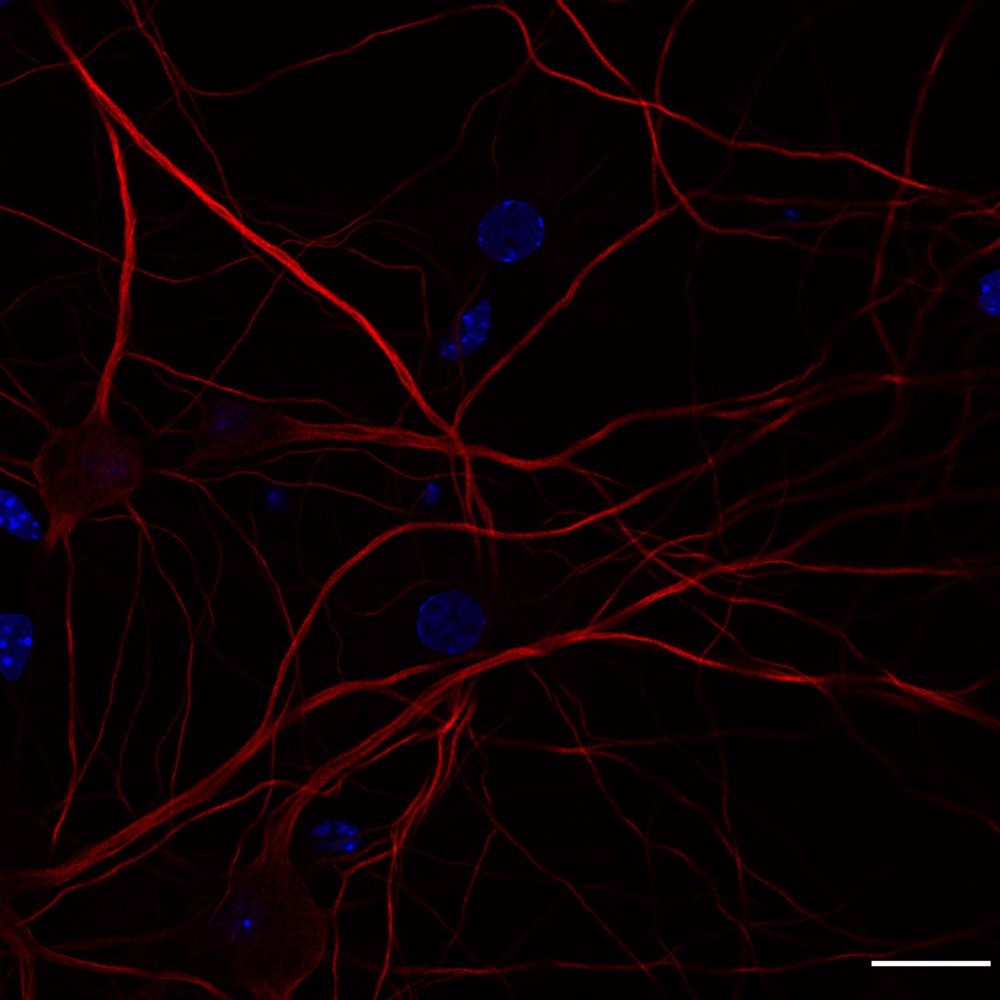
\includegraphics[width=\textwidth]{./Images/Immuno/Musk/Cultures/MAP2_20um.jpg}
		\end{subfigure}
		\begin{subfigure}[h]{0.329\textwidth}
			\caption{}
			\label{fig:CultureMMmap2musk}
			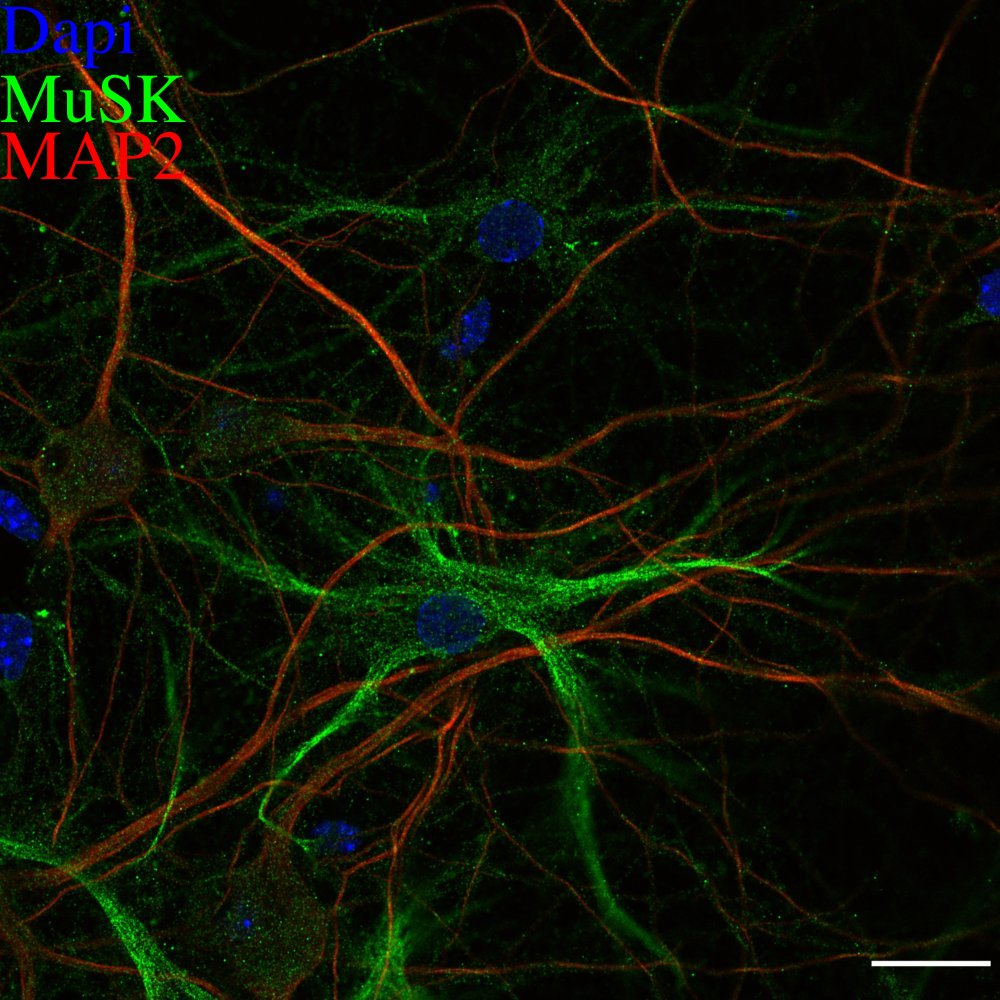
\includegraphics[width=\textwidth]{./Images/Immuno/Musk/Cultures/MuSK-MAP2_20um.jpg}
		\end{subfigure}
	\caption{Co-marquage de \gls{musk} et \gls{gfap} (astrocytes) ou \gls{musk} et \gls{map2} (neurones) sur une culture d'hippocampe.}
	\descfig{%
					Co-marquage de \gls{musk} (vert), \acrshort{dapi} (bleu) et \gls{map2} (rouge, \subref{fig:CultureMMmusk}-\subref{fig:CultureMMmap2musk}) et \gls{gfap} (rouge, \subref{fig:CultureMGmusk}-\subref{fig:CultureMGgfapmusk}).
					\subref{fig:CultureMGmusk} Marquage de \gls{musk}
					\subref{fig:CultureMGgfap} Marquage de \gls{gfap}
					\subref{fig:CultureMGgfapmusk} Merge 
					\subref{fig:CultureMMmusk} Marquage de \gls{musk}
					\subref{fig:CultureMMmap2} Marquage de \gls{map2}
					\subref{fig:CultureMMmap2musk} Merge. Flèches blanches : marquage cytoplasmique de \gls{map2} et de \gls{musk}.
					Barre d'échelle : 50µm (\subref{fig:CultureMGmusk}-\subref{fig:CultureMGgfapmusk}) ; 20µm (\subref{fig:CultureMMmusk}-\subref{fig:CultureMMmap2musk}).
					}
	\label{fig:MuSKMAP2GFAP}
	\end{figure}
	\FloatBarrier

\section{Immunoprécipitation}
\label{sec:IPresultat}
	Afin de confirmer la détection de \gls{musk} dans diverse région du cerveau, une immunoprécipitation suivie d'un \gls{wb} a été réalisée sur trois structures : l'hippocampe, le cervelet et le cortex de trois souris C57Bl/6 sauvage. Un \gls{wb} de \gls{musk} a déjà été réalisée par une autre équipe à partir de diverses structures du cerveau \cite{Garcia-Osta2006}, mais à partir d'extrait total de protéines et non d'une \gls{ip}, et avec des anticorps primaires différents. Une bande correspondante à \gls{musk} était révélé, bien que faible. Durant son stage, B. Somon a tenté de réaliser un \gls{ip} suivi d'un \gls{wb}, mais sans obtenir de résultats probant. Ici, la principale modification apportée au protocole précédemment utilisée par cette étudiante est l'utilisation de tampon RIPA (adjonction de déoxycholate de sodium et de \acrshort{sds} dans le tampon) qui permet une meilleure lyse et une meilleure préservation des protéines lors de l'extraction.
	
	Afin de vérifier si la technique fonctionnait, j'ai tout d'abord prélevé l'hippocampe, le cervelet et le cortex de trois souris C57Bl/6 puis réalisé une \gls{ip} de \gls{musk} à partir de ces tissus, qui a ensuite été migré dans un gel pour un \gls{wb}. En première expérience, comme l'anticorps utilisé pour l'\gls{ip} et la révélation était le même, un anticorps secondaire ciblant uniquement les chaines légères a été utilisé, afin d'éviter d'avoir trop de marquage non spécifique. Cependant, rien ne fut révélé, même le témoin positif étant très faible malgré un temps d'exposition important (supérieur à 30 minutes) (\cref{fig:WB-anti-LC}). Pour une deuxième expérience, la membrane a alors été deshybridée puis ré-incubée avec de l'anti-\gls{musk} ainsi qu'un autre anticorps secondaire dirigé contre les chaînes légères et lourdes d'\Glspl{ig} de lapin, qui à pour défaut d'être plus bruité (bande à 75kDa correspondant aux anticorps non couplés lors de l'\gls{ip}), mais qui permet de mieux révéler les bandes faiblement exprimées. De façon surprenante, des bandes de taille attendue (110kDa) ont été révélées dans l'hippocampe et le cervelet (\cref{fig:WBbon}, flèches noires), alors que dans le cortex une bande d'intensité plus faible semblait être présente (\cref{fig:WBbon}, tête de flèche noire), ce qui pourrait correspondre au fait qu'il n'y ait pas dans cette région du cerveau de marquage de \gls{musk} par \gls{ihc}. 
	
	Comme la taille des bandes ne correspondaient pas tout à fait à celle du témoin positif (extrait de cellules HEK293 transfectées avec un ADNc de \gls{musk}, à 130kDa, \cref{fig:WBbon}, flèche blanche), une troisième expérience a été réalisée avec des souris \mcrd et sauvages, issues de la même lignée. En effet, suite à la mutation, la protéine \gls{musk} à un poids moléculaire attendu de ~80kDa : si c'est bien \gls{musk} qui est détecté, on devrait alors avoir un décalage de poids entre les bandes. Cette fois-ci cependant, l'expérience ne s'est pas montrée concluante, rien n'a été révélé (\cref{fig:WB1erechec}). Enfin, afin de confirmer ce résultat, une quatrième et dernière expérience a finalement été tentée, avec comme témoin positif les extraits protéiques de la deuxième expérience (cervelet et cortex, plus assez d'extraits d'hippocampe pour recommencer). Aucun signal n'a été révélé, ni dans la troisième, ni dans la quatrième expérience(\cref{fig:WB1erechec}, \cref{fig:WBpasbon}).
	
	%Western Blot	
	\begin{figure}[h]
		\begin{center}
			\begin{subfigure}[h]{0.49\textwidth}
				\caption{}
				\label{fig:WB-anti-LC}
				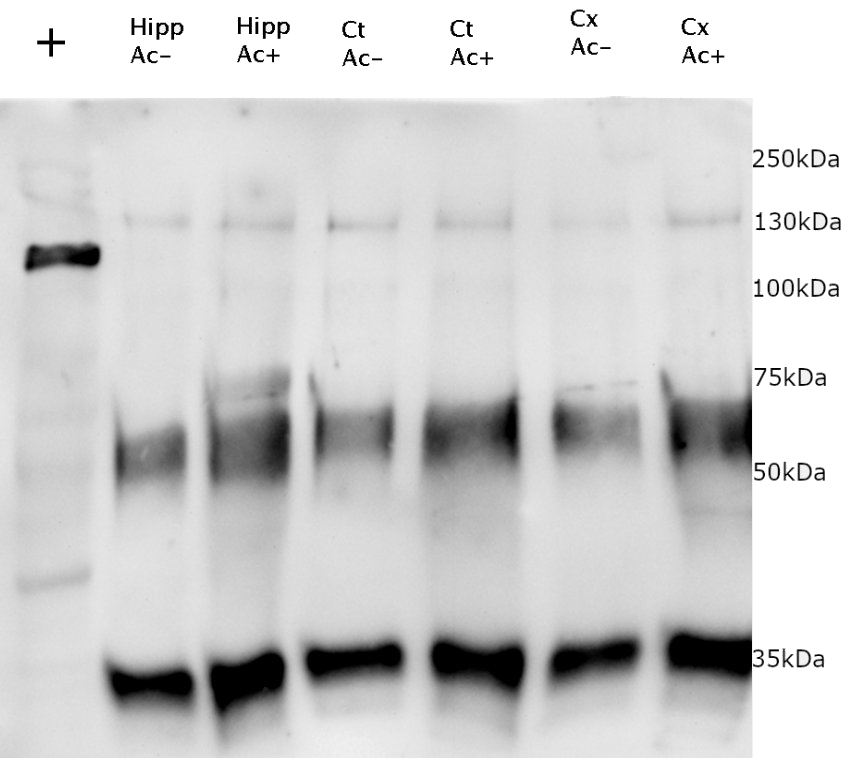
\includegraphics[width=\textwidth]{./Images/WB/@LC_MuSK_30'.jpg} %Gel anti light chain
			\end{subfigure}
			\begin{subfigure}[h]{0.49\textwidth}
				\caption{}
				\label{fig:WBbon}
				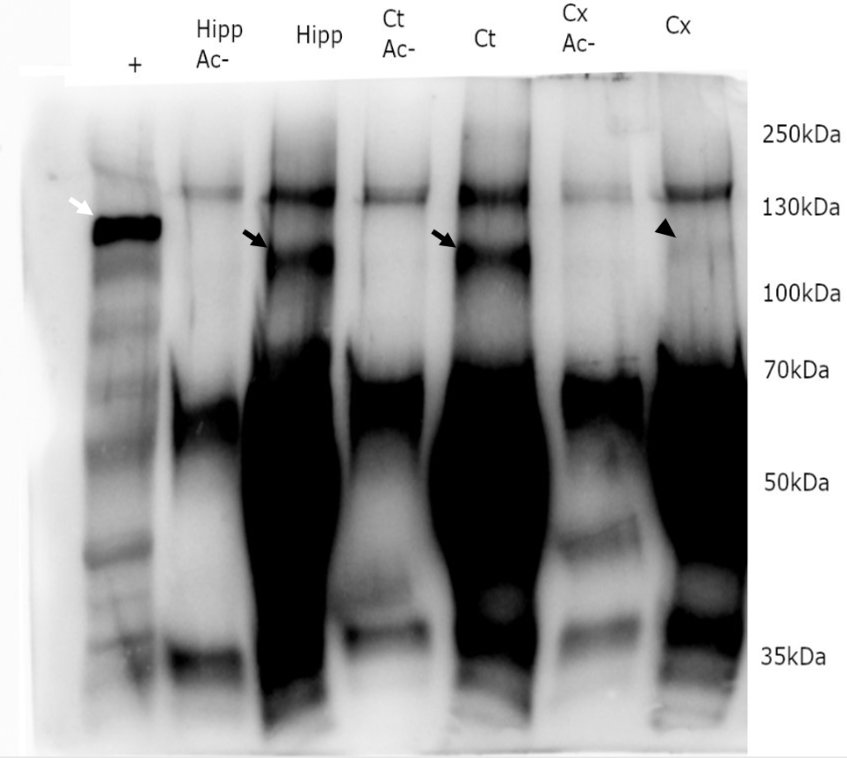
\includegraphics[width=\textwidth]{./Images/WB/2018-04-09.jpg} %Gel Bon :)
			\end{subfigure}
			\begin{subfigure}[h]{0.49\textwidth}
				\caption{}
				\label{fig:WB1erechec}
				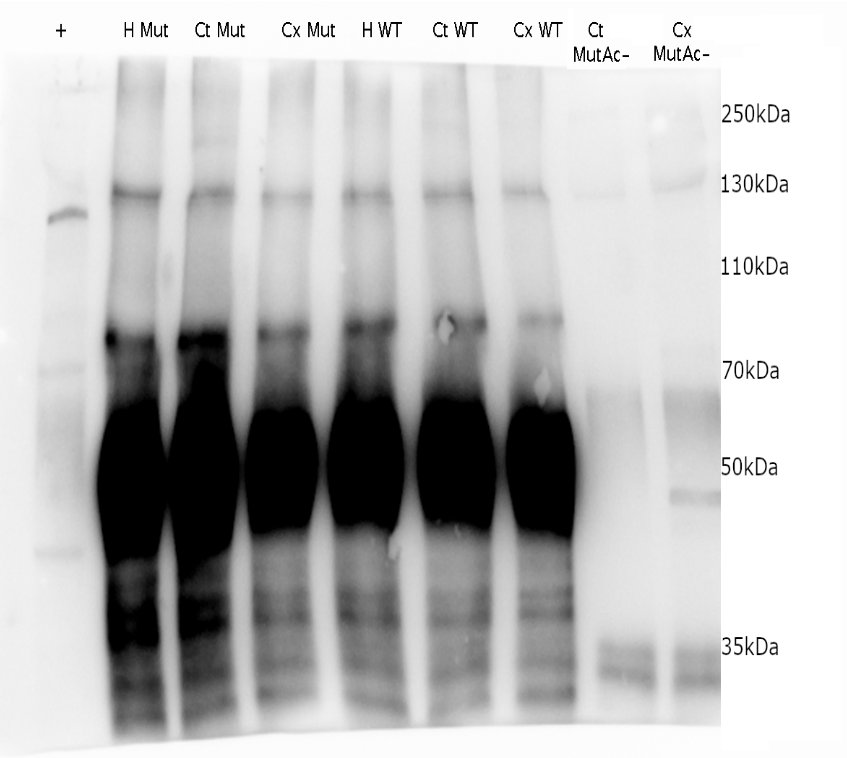
\includegraphics[width=\textwidth]{./Images/WB/2018-04-19.jpg} %Gel pas bon :(
			\end{subfigure}
			\begin{subfigure}[h]{0.49\textwidth}
				\caption{}
				\label{fig:WBpasbon}
				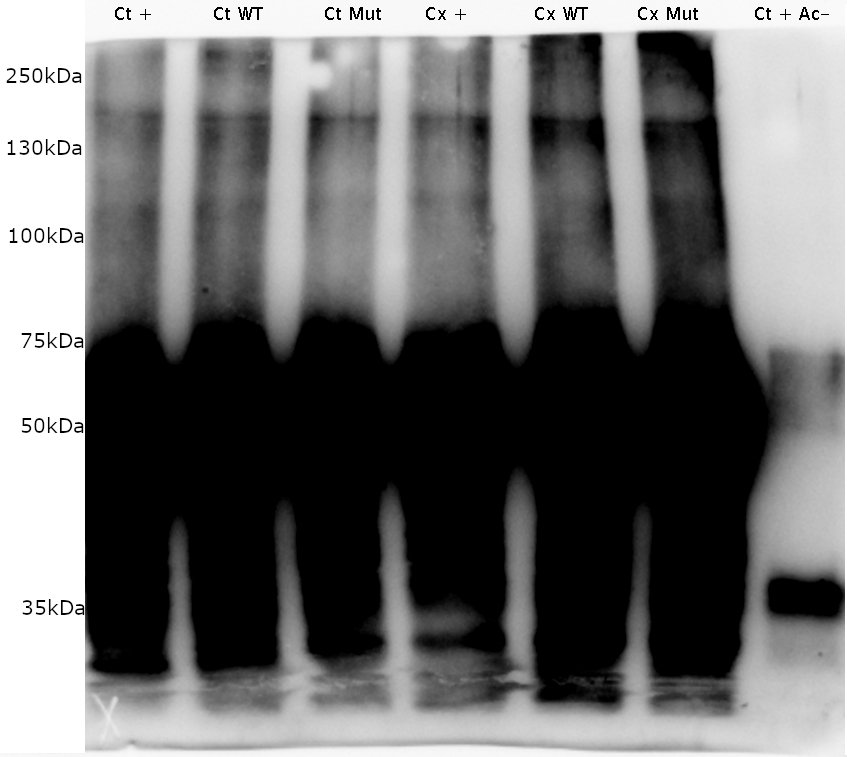
\includegraphics[width=\textwidth]{./Images/WB/2018-05-03.jpg} %Gel pas bon :(
			\end{subfigure}
		\end{center}
		\caption{L'\gls{ip} de \gls{musk} ne permet pas de confirmer la présence de \gls{musk} dans différentes structures du cerveau.}
		\descfig{%
			\subref{fig:WB-anti-LC} \gls{ip} suivie suivie de \gls{wb} sur 3 souris C57BL/6 révélée avec un anticorps dirigée contre les chaînes légères d'\gls{ig} de lapin. Seule la bande témoin au alentours de 130kDa est révélée. Exposition : 30 minutes. %
			\subref{fig:WBbon} \gls{ip} suivie de \gls{wb} sur 3 souris C57BL/6. Des bandes sont révélés aux alentours de 110kDa pour les régions de l'hippocampe et du cervelet (flèches noires). Une bande de faible intensité semble être présente pour le cortex (tête de flèche noire). Témoin positif : 15µL d'extrait cellulaire de cellules HEK293 transfectées, bande à 130kDa (flèche blanche). Exposition : 3 minutes. %
			\subref{fig:WB1erechec} \gls{ip} suivie de \gls{wb} sur 3 souris \mcrd (Mut) et 3 souris sauvages (WT) issues de la même souche. Exposition : 3 minutes.
			\subref{fig:WBpasbon} \gls{ip} suivie de \gls{wb} sur 3 souris \mcrd (Mut) et 3 souris sauvages (WT) issues de la même souche. Aucune bande n'est révélée, avec ou sans anticorps durant \gls{ip}. Aucune bande n'est révélé non plus chez le témoin positif : Extrait de cervelet et cortex issus de la première expérience. Hipp : Hippocampe, Ct : Cervelet, Cx : Cortex, + : Témoin positif, Ac- : Sans anticorps lors de l'\gls{ip}, Mut : Mutant, \acrshort{wt} : Sauvage. Poids moléculaire de \gls{musk} attendu : 110kDa. Exposition : 3 minutes. %
				}
		\label{fig:WBResultat}
	\end{figure}
\FloatBarrier

\section{Expression de \acrshort{musk} et \mcrd dans le cerveau}
\label{sec:ExpressionMuSK}
	Afin de tester l'impact potentiel de la delétion du \gls{crd} sur l'expression de la protéine, j'ai réalisé une \gls{qpcr} sur trois structures différentes : le cervelet, l'hippocampe gauche et droit. En effet, des résultats très préliminaires dans le laboratoire chez des 2 souris sauvages de souche C57Bl/6 (1 mâle et 1 femelle) avaient montrés une légère différence d'expression selon l'hémisphère du cerveau étudié. De plus, on retrouvait également une différence d'expression de \gls{musk} entre des individus de sexe opposé. Mon objectif a donc été de confirmer les différences d'expressions liées au genre et à l'hémisphère chez les souris \gls{wt} et de tester ces mêmes paramètres chez les souris \mcrd.
	
	Par manque d'individus au moment de l'expérience, je n'ai pas pu tester les conditions mâles \emph{versus} femelles, mais uniquement la différence d'expression du récepteur entre les structures. Concernant la différences d'expression entre ces régions du cerveau, j'ai pu constaté que chez les individus \gls{wt} (\cref{fig:qPCRCompaWT}), \gls{musk} était plus exprimé dans l'hippocampe gauche que dans l'hippocampe droit (p-value : 0.0453) ou dans le cervelet (p-value : 0.0462). La différence d'expression entre l'hippocampe droit et le cervelet n'est pas significative (p-value : 0.0648).
	
	Pour l'expression de \mcrd, une confusion de ma part entre les informations du fournisseur des primers (Qiagen\texttrademark) et une base de données (Gene, NCBI) ne m'a pas fait réaliser à temps que les primers s'hybridaient au niveau de la région du \gls{crd}, d'où une absence d'expression lors de la \gls{qpcr}. 
	
	\begin{figure}[h]
		\begin{minipage}{0.5\textwidth}
			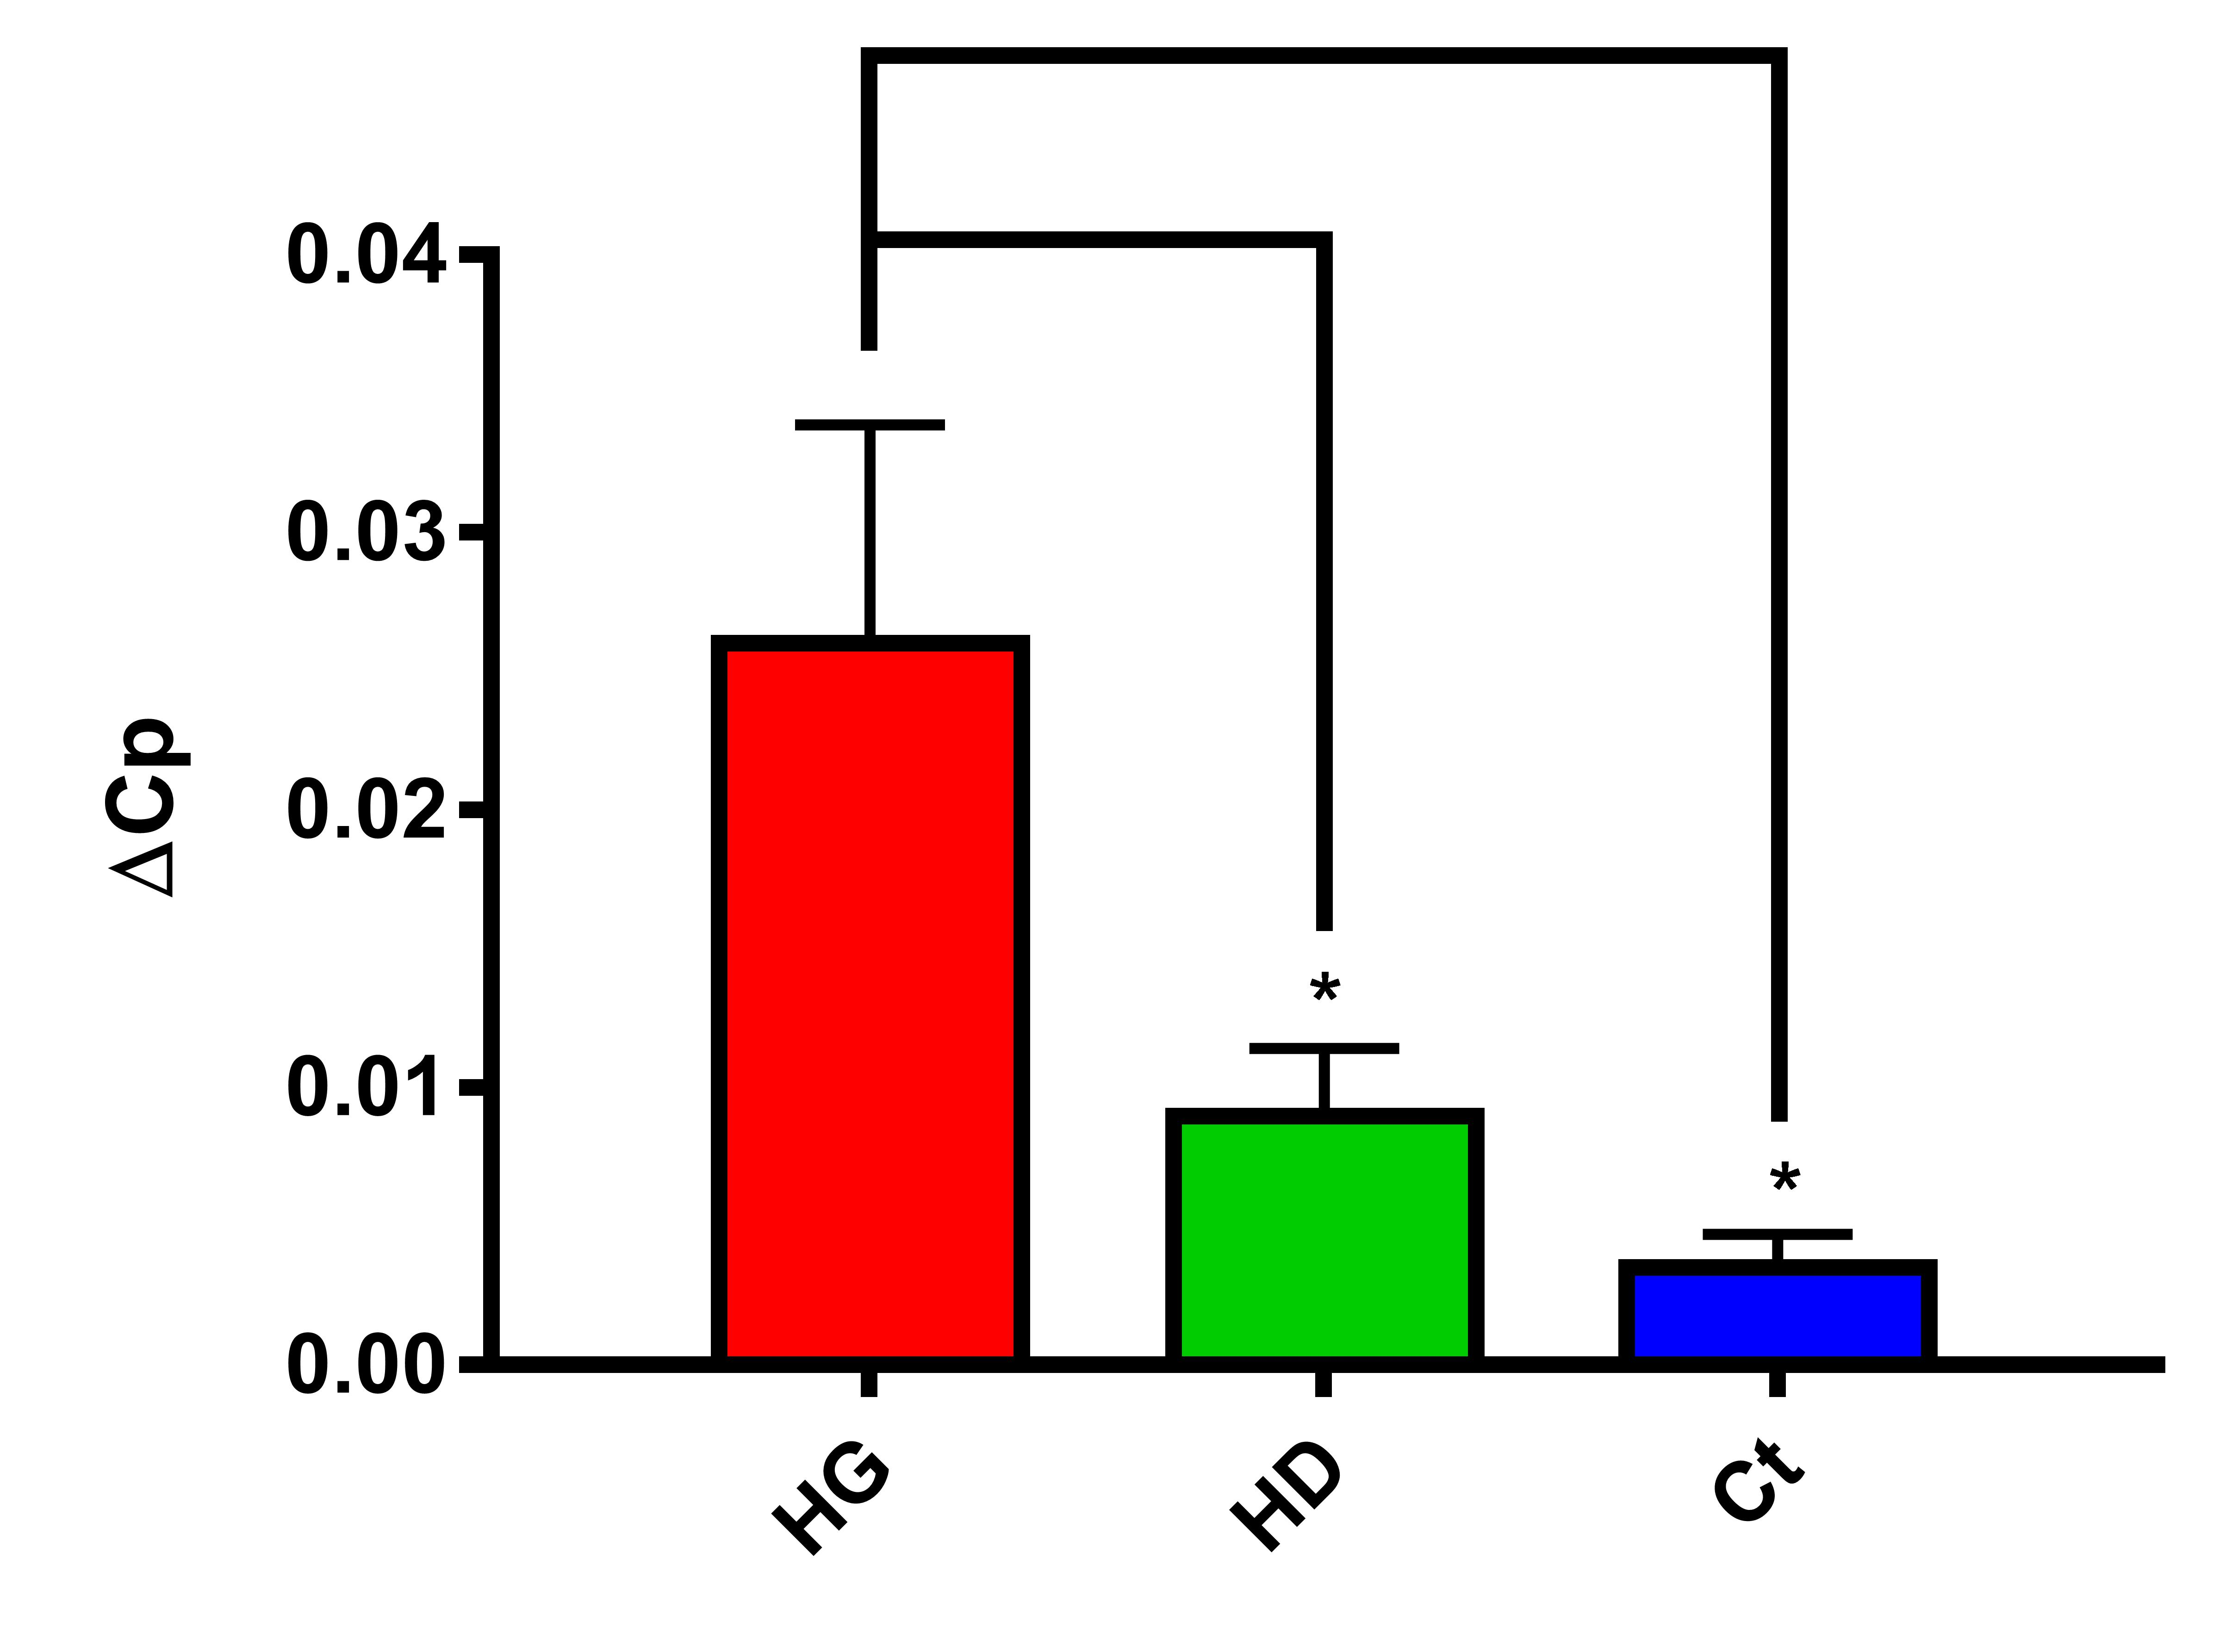
\includegraphics[width=\textwidth]{./Images/qPCR/Comp_Struct_WT.jpg}
		\end{minipage}%	
		\begin{minipage}{0.5\textwidth}
			\caption{L'expression de \gls{musk} varie entre l'hippocampe gauche et droit chez la souris.}
			\descfig{Comparaison de l'expression de \gls{musk} dans différentes structures chez les individus sauvages. %
				HG : Hippocampe Gauche, HD : Hippocampe Droit, Ct : Cervelet. n = 3 (\gls{wt}). %
				Test statistique : Test t de Student apparié. %
				* : p<0.05, ** : p<0.01, *** : p<0.001. %
			}
			\label{fig:qPCRCompaWT}
		\end{minipage}%	
	\end{figure}
%	\FloatBarrier

\section{Comportement}
\label{sec:Comportement}
Concernant les blessures préalablement observées sur les souris \mcrd mâles lors du stage de B. Somon, elles n'ont pas pu être reproduites durant mon stage, alors que les animaux provenaient de 2 animaleries différentes, celle de la plateforme locale du site des Saints Pères et celle de l’ICM (Institut du Cerveau et de la Moëlle, Paris). Les animaux (mutants comme hétérozygotes) ont cependant été qualifiés de "plus sensible à leurs environnement que la normale" par les animaliers en charges de ceux-ci. On peut faire l'hypothèse que durant le stage de B. Somon, les souris, qui étaient à l'époque élevée dans une ancienne animalerie, étaient soumises à un stress plus important. Ce stress pourrait expliquer un comportement d'automutilation/hypergrooming chez les souris mutantes. 
\FloatBarrier %Empeche figures etc d'aller dans chap. suivants

\chapter{Discussion}
Grâce aux co-marquage de \gls{musk} et \gls{gfap}, j'ai pu montré que dans le cerveau, \gls{musk} est exprimé par les astrocytes. Cependant,  un doute reste sur la spécificité du marquage de l'anticorps anti-\gls{musk}. Hessert \emph{et al.} en 2006 ont généré une lignée de souris \gls{musk}/LoxP croisée avec une souris où le gène de la recombinase Cre est sous promoteur de la créatine kinase \cite{Hesser2006}. Dans cette souris Cre/LoxP, \gls{musk} est inactivé dans les cellules musculaires au cours du développement, à la différence des souris KO. On peut alors imaginer croiser la lignée \gls{musk}/LoxP avec une lignée de souris Cre sous contrôle d'un promoteur nerveux (exprimé à la fois par les neurones et par les cellules glial) pour obtenir un modèle de souris \gls{musk} KO spécifique du cerveau. Cette lignée permettrait d'étudier l'effet du récépteur dans le cerveau, et permettrait également de confirmer la spécificité du marquage.

Un autre moyen de confirmer le marquage de \gls{musk} serait de réaliser un co-marquage avec un autre anticorps dirigé contre le récepteur. J'ai appris récemment l'existence d'un tel anticorps utilisé par l'équipe de Lin Mei, utilisable en immunofluorescence. Le co-marquage de deux anticorps dirigé contre deux régions différentes du récepteur serait un bon indice sur la spécificité du marquage. 

Pour l'expression de \gls{musk}, de nombreux gènes sont exprimés de manière différentes entre les deux hémisphères, notamment entre les deux hippocampes \cite{Moskal2006}. Cette asymétrie Gauche-Droite est un processus essentiel notamment à la formation de la mémoire \cite{Shimbo2018}. \gls{musk} suit asymétrie et apparaît plus fortement exprimé dans l'hippocampe gauche que dans l'hippocampe droit. Cependant, cette tendance ne ressort par chez les souris mutante. Mais le gène chez ces dernière s'est amplifié tard (après le 35\up{ème} cycle). Ces résultats ne sont donc pas en eux-mêmes interprétable. Il ne serait pas inenvisageable que ce qui ai été amplifié soit du bruit de fond. Cependant, on peut voir que la différence avec les souris sauvages est notable. On peut donc poser deux hypothèse : Soit effectivement, l'expression de \gls{musk} est fortement réduite chez les mutants, soit la mutation empêche l'appariement des primers sur le gène. Ces primers fournis par Qiagen\texttrademark sont propriétaire et leur séquence exacte n'est pas connue. Cependant, la région où les primers s'accrochent est éloignée de 1000pbs de la région du \gls{crd}, donc cette dernière hypothèse est peu probable.

Il serait interessant de voir l'évolution de l'expression de \gls{musk} au cours du développement : on pourrait alors faire des \gls{qpcr} à différents stades embryonnaire et néo-natal.

Comparaison Immuno/qPCR
Cultures
Hypothèse rôle Musk
Tempéré résultats neun : taille effet ? n suffisant ? variations lors coupes/mesures.
 A finir
\FloatBarrier %Empeche figures etc d'aller dans chap. suivants

\chapter{Perspectives}
Concernant l'organisation de l'hippocampe, je ne me suis intéressé qu'a la répartition des neurones dans l'hippocampe, et non à la densité cellulaires. Il pourrait être intéressant de comparer celle-ci entre des individus sauvages et mutants. De plus, le Gyrus Denté étant l'un des lieu de neurogenèse chez la souris adulte, et les \gls{wnt} étant impliquées dans la mémoire, il serait intéressant de faire une étude sur cette neurogenèse au travers un marquage au \gls{brdu}, afin de voir si celle-ci est perturbée chez la souris adulte mutante.

Un marquage de \gls{musk} par un autre anticorps pourrait permettre de lever le doute sur la spécificité de ce que j'ai pu observé. J'ai appris récemment que l'équipe de Lin Mei (Georgie, USA) possédait un anti-\gls{musk} utilisable en immunofluorescence. Je ne connais cependant pas quelle partie du récepteur cet anticorps reconnait.

Pour poursuivre l'études du rôle de \gls{musk} et des conséquences de la mutation \mcrd, l'étape suivante serait de réaliser des tests comportementaux, en collaboration avec une plateforme spécialisée de l'ICM. Ces tests permettraient d'observer les effets sur la mémoire, l'orientation spatiale, et le stress, de la mutation de \gls{musk}.

Sun \emph{et al.} avaient décrit la présence de \gls{musk} dans les astrocytes et les neurones par \gls{qpcr}. Les cellules provenaient d'embryon au stade E18. Ici, j'ai étudié l'expression de \gls{musk} chez des souris agées de 30 jours. Il serait intéressant d'observer l'évolution de l'expression de \gls{musk} au cours du développement, au moyen de \gls{qpcr} réalisés à différents stades embryonnaire et post-nataux. De plus, il faudrait produire des primers de \gls{qpcr} qui ne s'hybride pas dans la région du \gls{crd}. 

%%%%% Inclusion Bibliographie %%%%%
\begingroup
\let\clearpage\relax
\printbibliography[heading=bibintoc, title=Références]
\endgroup
\clearpage

%Résumé 10 lignes
\cfoot{ }
\chapter*{Résumé}\thispagestyle{fancy}
\addcontentsline{toc}{chapter}{Résumé}
\Acrshort{musk} est un récepteur tyrosine kinase connut pour son rôle crucial dans la formation et la maintenance de la jonction neuromusculaire. Ce récepteur est activé par 3 ligands : l’agrine, \acrshort{colq}  et les \acrshortpl{wnt}. Ces dernières se lient sur un domaine \acrshort{crd} dans l’ectodomaine de \acrshort{musk} nécessaire à la synaptogenèse. Cependant, le rôle de MuSK et du domaine CRD dans le cerveau reste méconnu. L'utilisation de techniques de coloration histologique, d'immunomarquage et de \acrshort{qpcr}, m'ont permis de montré que le récepteur \acrshort{musk} est localisé dans des endroits discrets du cerveau (Hippocampe notamment) et est exprimé par des astrocytes de type fibreux. De plus, le \acrshort{crd} participe à la structuration des couches neuronales de l'hippocampe. Enfin, je montre que le récepteur est exprimé différemment par l'hippocampe gauche ou droit. Ce travail est le premier à s'intéressé spécifiquement à la localisation cellulaire de la protéine \acrshort{musk} et représente un premier pas dans l'étude du rôle comportementale du récepteur.

\end{document}